\documentclass[a4paper,12pt,twoside]{book} 
\usepackage[utf8]{inputenc}

\usepackage{listings}
\usepackage{xcolor}

%New colors defined below
\definecolor{codegreen}{rgb}{0,0.6,0}
\definecolor{codegray}{rgb}{0.5,0.5,0.5}
\definecolor{codepurple}{rgb}{0.58,0,0.82}
\definecolor{backcolour}{rgb}{0.95,0.95,0.92}

%Code listing style named "mystyle"
\lstdefinestyle{mystyle}{
  backgroundcolor=\color{backcolour},   commentstyle=\color{codegreen},
  keywordstyle=\color{magenta},
  numberstyle=\tiny\color{codegray},
  stringstyle=\color{codepurple},
  basicstyle=\ttfamily\footnotesize,
  breakatwhitespace=false,         
  breaklines=true,                 
  captionpos=b,                    
  keepspaces=true,                 
  numbers=left,                    
  numbersep=5pt,                  
  showspaces=false,                
  showstringspaces=false,
  showtabs=false,                  
  tabsize=2
}

%"mystyle" code listing set
\lstset{style=mystyle}

% standard incantations
\usepackage[T1]{fontenc}
\usepackage[utf8]{inputenc}
\usepackage{lmodern}
\usepackage[german]{babel}
\usepackage{csquotes}

% clickable links in the PDF
\usepackage{hyperref}
\usepackage{float}
% bibliography
\usepackage[sorting=none]{biblatex}
\addbibresource{literatur.bib}

% glossary
\usepackage[xindy]{glossaries} 
\newglossaryentry{souveraenitaet}{%
  name={Souveränität},%
  description={Der Begriff Souveränität, auch „Staatshoheit“, wird im innerstaatlichen Recht und in der politischen Theorie verwendet, um die oberste Kompetenz zur Machtausübung im Innern eines Staates zu bezeichnen\cite{grundgesetzSouv}.}}

\newglossaryentry{kks}{%
  name={KKS},%
  description={künstliche Währung zum Ausgleich von Preis­niveau-Unterschieden zwischen den Mitgliedstaaten der Europäischen Union; ein Kaufkraftstandard (KKS) entspricht der durchschnittlichen Kaufkraft eines Euro in der Europäischen Union (EU-27)}}

\newacronym{eu}{EU}{Europäische Union}

% generic
\newacronym{afd}{AfD}{Alternative für Deutschland}
\newacronym{zdf}{ZDF}{Zweites Deutsches Fernsehen}
\newacronym{api}{API}{Application Programming Interface}
\newacronym{ai}{AI}{Angewandte Informatik}
\newacronym{ip}{IP}{Internet Protocol}
\newacronym{ssh}{SSH}{Secure Shell}
\newacronym{cli}{CLI}{Command Line Interface}
\newacronym{htw}{HTW}{Hochschule für Technik und Wirtschaft}
\newacronym{xml}{XML}{Extensible Markup Language}
\newacronym{json}{JSON}{JavaScript Object Notation}
\newacronym{sob}{SoB}{Sentiments of Bundestag}
\newacronym{rest}{REST}{Representational State Transfer}
\newacronym[plural=MDBs, firstplural=Mitglieder des Deutschen Bundestages (MDBs)]{mdb}{MDB}{Mitglied des Deutschen Bundestages}

% group 2
\newacronym{cme}{CME}{Communication Model Extractor}


\makeglossaries

% add literatur to toc
\usepackage[nottoc]{tocbibind}

% graphics and images
\usepackage{graphicx}
\usepackage{subfigure}
\usepackage{wrapfig}

% color packages
\usepackage{color, colortbl}
\definecolor{Gray}{RGB}{220,220,220}
\definecolor{EUBlue}{RGB}{45,172,227}
\definecolor{White}{RGB}{255,255,255}
\usepackage[first=0,last=9]{lcg}
\newcommand{\ra}{\rand0.\arabic{rand}}

% multirow table
\usepackage{multirow}

% footnote package
\usepackage{tablefootnote}

\lstset{
  captionpos=b,
  commentstyle=\color{UStuttDarkGreen},
  frame=single,	                   % adds a frame around the code
  keepspaces=true,
  %keywordstyle=\color{UStuttDarkBlue},
  showspaces=false,
  showstringspaces=false,          % underline spaces within strings only
  showtabs=false,
  stringstyle=\color{UStuttDarkBlue},
  tabsize=2
}

% --------------------------------------------------------------------
% Definitions of title informations
% --------------------------------------------------------------------
\newcommand{\HRule}[1]{\rule{\linewidth}{#1}}

\makeatletter
\def\printtitle{	
    {\centering \@title\par}}
\makeatother			

\makeatletter
\def\printauthor{
    {\centering \large \@author}}
\makeatother

% --------------------------------------------------------------------
% Config Title & Author
% --------------------------------------------------------------------
\title{
\HRule{0.5pt} \\
\LARGE \textbf{\uppercase{Sentiments of Bundestag}}
\HRule{2pt} \\ [0.5cm]
\normalsize \textsc{Graph-basiertes Informationssystem zur Analyse sozialer Interaktion im Deutschen Bundestag}
\\[2.0cm]
\normalsize \today
}

\author{
\normalsize Betreut von
\normalsize Prof. Dr. Thomas Hoppe\\
\normalsize Informationssysteme\\
\normalsize M.Sc. Angewandte Informatik\\
\normalsize Hochschule für Technik und Wirtschaft\\
\normalsize Treskowallee 8, 10318 Berlin, Deutschland\\
}

\begin{document}
% ------------------------------------------------------------------------------
% Maketitle
% ------------------------------------------------------------------------------
\thispagestyle{empty}
\printtitle
  	\vfill
\begin{figure}[H]
    \centering
    
\includegraphics[width=200px, keepaspectratio]{logos/bundestag.png}
\end{figure}
  	\vfill
\printauthor		
\newpage

\pagenumbering{roman}
\setcounter{page}{3}

\setcounter{tocdepth}{2}
\tableofcontents

\listoffigures

\listoftables

\pagenumbering{arabic}
\setcounter{page}{6}

\chapter{Vorwort}
\section{Einleitung}
Der Begriff \textit{Sentiment} stammt vom lateinischen Wort \textit{sentimentum} ab und bedeutet Empfindung oder Stimmung. 
In der Sentimentanalyse geht es um die Bestimmung eben jener Stimmung einer Meinungsäußerung. 
Anwendung findet sie etwa bei Produktbewertungen oder Beiträgen in sozialen Netzwerken. 
Die Stimmung wird durch die sog. Polarität beschrieben und kann positiv, negativ oder neutral ausfallen. 
Im Text-Mining wird sie im Intervall $\interval{-1}{1} = \{x \in \mathbb{R} | -1 \leq x \leq 1\}$ angegeben, wobei -1 sehr negativ, 1 sehr positiv und 0 neutral bedeuten. 

Grundlegend ist die maschinelle Sentimentanalyse entweder Wortlisten- oder Modell-basiert. 
Der Wortlisten-Ansatz kann als eine Sammlung von Worten und ihrer Polaritäten verstanden werden, anhand welcher die Stimmung berechnet wird. 
Dieser Ansatz wird weiter im Kapitel \ref{wortliste} beschrieben, da er in dieser Arbeit verwendet wurde. 

Bei der Modell-basierten Sentimentanalyse wird ein annotierter Satz-Korpus für das Trainieren einer künstlichen Intelligenz vorausgesetzt. 
Etwa für Twitter-Beiträge stehen solche Korpusse oder auch bereits trainierte Modelle zur Verfügung. 
Jedoch ist bei der Verwendung zur Analyse der Sitzungsprotokolle des Bundestages nicht mit zufriedenstellenden Ergebnissen zu rechnen, da sich verwendete Worte und Text- bzw. Satzbau zwischen diesen Domänen deutlich unterscheiden. 
Eine weitere Erläuterung zur Sprache im Bundestag wird in Kapitel \ref{sprachebundestag} gegeben. 

Ebenfalls werden die Komponenten zur Teilnahme an der Verarbeitungspipeline des Gesamtprojektes im nachfolgenden Kapitel \ref{g3daten} beschrieben. 

\section{Datenaustausch}
\label{g3daten}
\subsection{Datenimport}
Für das Erhalten von Daten wurde eine Methode implementiert, welche durch Angabe einer Sitzungs-ID die entsprechende Sitzung vom REST-API von Gruppe 2 abfragen kann. 
Diese Methode gibt jede Sitzung weiter an die in Kapitel \ref{g3textv} beschriebene Textverarbeitung und das Ergebnis schließlich an den in Kapitel \ref{g3export} beschriebenen Export-Code. 

Die Methode wird für zwei Fälle verwendet: 
Beim Normalfall sendet die Gruppe 2 eine Benachrichtigung mit einer Liste aller neuen Sitzungs-IDs an das REST-API im Code dieser Arbeit. 
Das REST-API wurde mit der Bibliothek \mintinline{latex}{Flask} \cite{g3_flask} entwickelt und besteht aus einer POST-Schnittstelle, welche auf dem von der HTW bereitgestelltem Server unter \textit{/notify} erreichbar ist. 

Das API wurde unter Zuhilfenahme von \mintinline{latex}{Flask.Blueprints} \cite{g3_flaskbp} entwickelt und wird von einem \mintinline{latex}{Waitress}-Webserver \cite{g3_waitress} bereitgestellt. 
Für jede Anfrage wird geprüft, ob Content-Type und Payload dem erwarteten JSON-Daten entsprechen. 
Sollte dies nicht der Fall sein, wird eine entsprechende Rückmeldung an den Sender zurückgegeben. 
Für jede erhaltene Sitzungs-ID wird die eingangs beschriebene Methode aufgerufen. 

Der zweite Fall wurde vor allem im Rahmen der voranschreitenden Entwicklung bei den in der Projektpipeline voranstehenden Gruppen verwendet. 
Statt auf eine Benachrichtigung zum Anstoßen des Datenimports zu warten, werden stattdessen alle Sitzungs-IDs vom REST-API der Gruppe 2 abgefragt und jede Sitzung vollständig neu importiert. 
Dieses Vorgehen hat den Vorteil, dass eventuell durch Arbeit am Code verpasste Benachrichtigungen nachgeholt werden und gleichzeitig Änderungen an den Daten übernommen werden können. 

\subsection{Datenexport}
\label{g3export}
Statt Arbeit in ein umfangreiches REST-API für die nachfolgenden Gruppen zu stecken, wurde für diese Arbeit ein reiner MongoDB-Ansatz verwendet. 
Auf dem zur Verfügung stehenden HTW-Server wurde dafür eine MongoDB Instanz aufgesetzt, welche nur aus dem HTW-Netz erreichbar und zudem nur mit Authentifizierung zugreifbar ist. 
Jede Sitzung ist hier als eine eigene Collection persistiert. 
Sobald neue Sitzungen importiert und verarbeitet wurden, werden diese zunächst mit dem MongoDB-Treiber \mintinline{latex}{PyMongo} \cite{g3_mongodb} in die Datenbank geschrieben. 
Anschließend werden die nachfolgenden Gruppen mit einem POST and die jeweilige REST-Schnittstelle benachrichtigt, dass neue Daten vorliegen. 
Diese greifen dann mit den zuvor versendeten Zugangsdaten direkt auf die Datenbank zu. 

Mit diesem Vorgehen konnte die Komplexität beim Zugriff auf die Ergebnis-Daten gesenkt werden, da es für nahezu alle gängigen Programmiersprachen einen intuitiven MongoDB-Treiber gibt. 

\section{Wortliste}
\label{wortliste}
Wie bereits in der Einleitung beschrieben, handelt es sich bei Wortlisten in der Sentimentanalyse um eine Liste von Worten und ihrer jeweiligen Polarität. 
Bei der Analyse eines Textes wird wortweise ein Abgleich mit dieser Liste durchgeführt und die Wort-Polarität bei einer Übereinstimmung für die Berechnung des Sentiments verwendet. 
Unterschiedliche Berechnungsformeln sind dabei denkbar und werden in Kapitel \ref{polberechnung} weiter besprochen. 
Für diese Arbeit wurden Wortlisten verschiedener Institutionen kombiniert und anschließend mit Synonymen erweitert. 
Ebenfalls wurde eine eigene Bundestags-Wortliste erstellt. 

Die Interest Group on German Sentiment Analysis (IGGSA) stellt eine umfangreiche Liste an Publikationen und Ressourcen zu Sentimentanalysen in der deutschen Sprache zur Verfügung \cite{g3_iggsa}. 
Hier wurden alle Referenzen auf die in dieser Arbeit verwendeten Quell-Wortlisten gesammelt. 
Für die Zusammenführung dieser Wortlisten wurden zunächst zwei Herangehensweisen evaluiert: 
Zum einen war die Erstellung eines eigenständigen Codes denkbar, welcher einmalig die Daten aus allen Quellen einliest, zusammenfasst und eine Ergebnis-Datei ausgibt. 
Diese Datei wäre eine Ressource für den eigentlichen Analyse-Code. 
Zum anderen könnte die soeben beschriebene Funktionalität jedoch auch direkt im Analyse-Code integriert und bei jedem Programmstart ausgeführt werden. 
Die kombinierte Wortliste würde somit nicht auf die Festplatte geschrieben, sondern im Arbeitsspeicher verbleiben, solange der Analyse-Code läuft. 
Wenngleich der zuerst beschriebene Ansatz offensichtlich weniger Rechenzeitaufwändig ist, wurde für diese Arbeit der zweite Ansatz gewählt. 
Dies wird vor allem mit Rechtsunsicherheiten bei der Arbeit mit den verschiedenen Lizenzen der Quelldateien begründet. 
Gleichzeitig arbeitet der Analyse-Code damit jederzeit mit dem aktuellen Stand der Quell-Wortlisten. 
Das Aufbauen der Wortliste dauert wenige Minuten. 

Für diese Arbeit wurden die folgenden Quell-Wortlisten verwendet: 

\begin{itemize}
\item \textit{SentimentWortschatz} (SentiWS) aus \glqq SentiWS - a Publicly Available German-language Resource for Sentiment Analysis\grqq (Universität Leipzig) \cite{g3_sentiws}
\item \textit{Multi-Domain Sentiment Lexicon for German} (Hochschule Darmstadt) \cite{g3_opm}
\item \textit{German Polarity Lexicon} aus \glqq Evaluation and extension of a polarity lexicon for German\grqq (Universität Zürich) \cite{g3_polcla}
\item \textit{morphcomp} aus \glqq Evaluating the morphological compositionality of pola-rity\grqq (Leibniz-Institut für Deutsche Sprache, Universität des Saarlandes) \cite{g3_morphcomp}
\end{itemize}

Aus diesen Quellen ergibt sich eine Wortliste mit etwa 14.000 einzigartigen Worten. 
Die Worte werden dabei mit der in Kapitel \ref{g3textv} beschriebenen Textverarbeitungspipeline lemmatisiert, also auf die Grundform zurückgeführt. 
Bei Überschneidungen wird ein Mittelwert über alle Polaritäts-Werte eines Wortes gebildet. 

Mithilfe des \textit{Open German WordNet} (OdeNet) \cite{g3_odenet} werden zu jedem Wort Synonyme gesammelt und ebenfalls der Wortliste hinzugefügt. 
Der Zugriff auf OdeNet geschieht dabei mit der python Bibliothek \mintinline{latex}{WN} \cite{g3_wn}. 
Die Verwendung dieser Bibliothek ist trivial, weshalb an dieser Stelle keine weitere Erläuterung gegeben wird. 
Die Wortliste wird durch das Hinzufügen von Synonymen um weitere rund 2.000 Worte erweitert. 

Wie bereits in der Einleitung erwähnt, wurde zudem eine eigene Bundes-tags-Wortliste erstellt. 
Hierzu wurden die 15.000 am häufigsten in den Sitzungsprotokollen vorkommenden Worte erfasst und analysiert. 
Dabei wurden jedoch nur jene Worte betrachtet, welche nicht bereits in der kombinierten Wortliste vorkommen. 
Ausgewählt wurden nur eindeutig positive oder negative Worte wie \textit{angemessen}, \textit{Bullshit}, \textit{Fehlentscheidung}, \textit{Milchmädchenrechnung}, \textit{Realitätsverweigerung}, \textit{Totalausfall} oder \textit{Verunglimpfung}. 
Insgesamt umfasst die Bundestags-Wortliste 217 Worte. 

Im Code wird der Zugriff auf die Wortliste mit der zentralen Klasse \mintinline{latex}{Lexicon} realisiert. 
Bei der Instanziierung der Klasse werden, wie im Vorherigen beschrieben, alle Wortlisten gesammelt, zusammengeführt und erweitert. 
Anschließend stellt die Klasse ein \mintinline{latex}{Dictionary} bereit, in welchem die Schlüssel die Worte und die Werte die Wort-Polarität angeben. 

\section{Textverarbeitung}
\label{g3textv}
Für die Textverarbeitung nutzt der Code dieser Arbeit vollständig die Funktionalitäten und Strukturen von \mintinline{latex}{spaCy} \cite{g3_spacy}. 
Die \mintinline{latex}{spaCy} Bibliothek stellt eine Textverarbeitungspipeline bereit, welche mithilfe eines vortrainierten Modells funktioniert. 
Für die deutsche Sprache wurde ein solches Modell mit dem TIGER Korpus der Universität Stuttgart trainiert. 
Der Korpus umfasst ca. 50.000 Sätze aus Texten der Frankfurter Rundschau. 
Die \mintinline{latex}{spaCy}-Pipeline besteht aus den folgenden Komponenten: 

\begin{itemize}
\item Tokenisierung (Text- und Satzzerteilung)
\item POS-Tagging (Wortartenerkennung)
\item Dependency-Parsing (Wortabhängigkeitenerkennung)
\item Lemmatisierung (Wortgrundformermittlung)
\item Entity-Recognition (Eigennamenerkennung)
\end{itemize}

Das Ergebnis der Pipeline ist ein \mintinline{latex}{Doc}-Objekt, welches das Ergebnis des gesamten in die Pipeline gegebenen Textes umfasst. 
Einzelne Sätze innerhalb des \mintinline{latex}{Doc}-Objektes werden mit \mintinline{latex}{Span}-Objekten beschrieben und einzelne Worte mit \mintinline{latex}{Token}-Objekten. 
Die Objekttypen besitzen jeweils eigene Methoden und Erweiterungsmöglichkeiten in Form von sog. \textit{extension attributes}. 

Sehr einfach und gleichzeitig umfangreich kann die \mintinline{latex}{spaCy}-Pipeline an die eigenen Bedürfnisse angepasst werden. 
So wurde die Berechnung des Sentiments eines Textes direkt an die Komponenten der Standart-Pipeline angehängt. 
Logisch unterteilt sich diese in die Komponenten:

\begin{itemize}
\item Negations-Erkennung (siehe \ref{neg-erkennung})
\item Verstärkungs-Erkennung (siehe \ref{ver-erkennung})
\item Polaritätsberechnung (siehe \ref{polberechnung})
\end{itemize}

Basis für das nachfolgende Kapitel \ref{neg-erkennung} ist dabei das Ergebnis des Depen-dency-Parsers von \mintinline{latex}{spaCy}. 
Dieser bestimmt die Abhängigkeiten zwischen den einzelnen Elementen eines Satzes. 
Diese Funktion gehört dem Themenbereich der Dependenzgrammatik an, in welcher gerichtete Beziehungen zwischen den Worten eines Satzes beschreibt werden. 
Ein Wort kann einen Vorgänger (Regent) und mehrere Nachfolger (Dependenten) besitzen. 
Die Gesamtheit der Beziehungen eines Satzes wird auch Abhängigkeitsbaum genannt. 

Zur Verdeutlichung soll die Abbildung \ref{steffi} dienen, welche mithilfe von \mintinline{latex}{spaCy.displaCy} erstellt wurde. 
Zu sehen ist hier der Abhängigkeitsbaum des Satzes \textit{\glqq Das ist doch fachlich Quatsch hoch sechs!\grqq}. 
An den gerichteten Kanten befindet sich die Angabe des Satzgliedes, unterhalb der Worte die Angabe der Wortart. 

\begin{figure}[htb]
\centerline{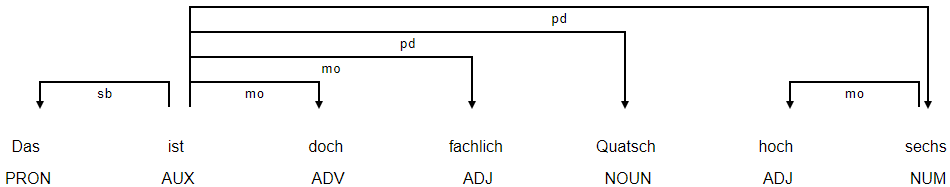
\includegraphics[width=1\textwidth]{chapters/04-Sentiment-Analyse/steffi.png}}
\caption{Visualisierung der Wortabhängigkeiten (Zitat von Steffi Lemke MdB, 208. Sitzung, 10.02.2021)}
\label{steffi}
\end{figure}

\subsection{Negations-Erkennung}
\label{neg-erkennung}
Negation, also Ablehnung, Verneinung oder Aufhebung, hat einen erheblichen Einfluss auf das Ergebnis und damit die Korrektheit der Sentimentanalyse, weshalb in dieser Arbeit ein besonderes Augenmerk auf ihre Erkennung gelegt wurde. 
In \textit{Negation Modeling for German Polarity Classification} \cite{g3_wieg} präsentieren Forscher der Universität des Saarlandes und des Leibniz-Institut für Deutsche Sprache hierfür einen regelbasierten Ansatz. 

Sie definieren unterschiedliche Negationstypen und ihre jeweilige Reichweite. 
So beeinflussen etwa negierende Adverbien oder Indefinitpronomen wie \textit{nie} den gesamten Satz, wohingegen das Partikel \textit{nicht} lediglich seinen Vorgänger negiert.  
Die Tabelle \ref{g3tab1} führt alle in dieser Arbeit implementierten Negationsregeln auf. 
Die Nutzung eines Abhängigkeitsbaumes, wie von \mintinline{latex}{spaCy} ermittelt, ist dabei unerlässlich. 
Denn wie schon im vorherigen Kapitel angesprochen, ist etwa mit dem Vorgänger eines Wortes nicht das in der Satzabfolge voranstehende Wort gemeint, sondern vielmehr der semantische Regent. 

\begin{table}[htbp]
\caption{Implementierte Negations-Regeln aus \cite{g3_wieg}}
\begin{center}
\begin{tabular}{| c | c | c |}
\hline
\textbf{Negationstyp} & \textbf{Reichweite} & \textbf{Beispielworte} \\ \hline
Partikel & Vorgänger (Regent) & nicht \\ \hline
Präpositionen & Nachfolger (Dependent) & ohne, gegen \\ \hline
Adverbien, & Satz & nie, kein, kaum \\
Indefinitpronomen &  &  \\ \hline
Nomen & Genitiv,& Abschaffung, \\
 & Präpositionalobjekt & Zerstörung \\ \hline
Verben & Objekt, Subjekt & enden, sinken, lindern \\
\hline
\end{tabular}
\label{g3tab1}
\end{center}
\end{table}

Angemerkt sei an dieser Stelle, dass es nicht möglich war, alle Regeln aus \cite{g3_wieg} zu implementieren, da der von den Forschern genutzte Dependency-Parser umfangreichere Ergebnisse liefert, als jener von \mintinline{latex}{spaCy}. 

Eine Liste mit Negationsworten und dem jeweiligen Negationstyp wurde \cite{g3_polcla} entnommen und ist ebenfalls über die Klasse \mintinline{latex}{Lexicon} zugreifbar. 
Die Klasse stellt ein \mintinline{latex}{Dictionary} bereit, in welchem die Schlüssel die Negationsworte und die Werte eine Liste der Reichweiten sind. 

Wenn in einem Text ein Negationswort auftritt, werden alle implementierten Regeln geprüft. 
Sollte es zu einem Treffer kommen, etwa wenn das Wort \textit{nicht} auftritt (siehe Abb. \ref{brandner}) und es einen Vorgänger gibt, werden alle Worte in Reichweite des Negationswortes negiert. 
Dies geschieht, indem für die jeweiligen Worte, welche wie in \ref{g3textv} beschrieben \mintinline{latex}{Token}-Objekte sind, ein eigenes Attribut mit der Bezeichnung \mintinline{latex}{negated} auf \mintinline{latex}{True} gesetzt wird. 
In der Polaritätsberechnung wird wortweise auf dieses Attribut geprüft und die Wort-Polarität bei einer Negierung mit -1 multipliziert. 

\begin{figure}[htb]
\centerline{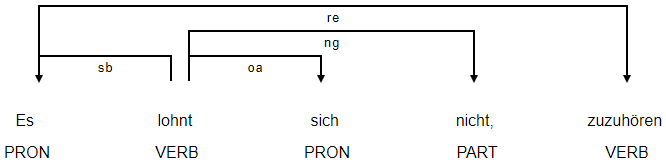
\includegraphics[width=1\textwidth]{chapters/04-Sentiment-Analyse/brandner.png}}
\caption{Beispielsatz mit Patikel-Negation (Zitat von Stephan Brandner MdB, 207. Sitzung, 29.01.2021)}
\label{brandner}
\end{figure}

\subsection{Verstärkungs-Erkennung}
\label{ver-erkennung}
Als \textit{Verstärker} werden sog. Gradpartikel (z.B. sehr, besonders, viel) verstanden, welche direkt vor Adjektiven oder Adverbien in einem Satz auftreten. 
Sie verstärken ihren Nachfolger, was wiederum in der Polaritätsberechnung berücksichtigt werden soll. 

Aus diesem Grund wird eine Liste mit verstärkenden Gradpartikeln, welche ebenfalls aus \cite{g3_polcla} bezogen werden, eingelesen und über die \mintinline{latex}{Lexicon} Klasse bereitgestellt. 

Ebenso wie in Kapitel \ref{neg-erkennung} bereits für die Negation beschrieben, wird ein eigenes Attribut zur Signalisierung einer Verstärkung definiert und im entsprechenden Fall auf True gesetzt. 
Bei der Polaritätsberechnung wird bei einer erkannten Verstärkung die Wort-Polarität mit 1,5 multipliziert \cite{g3_sentia}. 

In Abbildung \ref{hessel} wird ein Beispiel für das Auftreten eines verstärkenden Gradpartikels gegeben. 
Hier verstärkt das Wort \textit{sehr} das negative Wort \textit{spät}, womit die errechnete Polarität stärker negativ ausfällt als ohne die Verstärkungs-Erkennung. 

\begin{figure}[htb]
\centerline{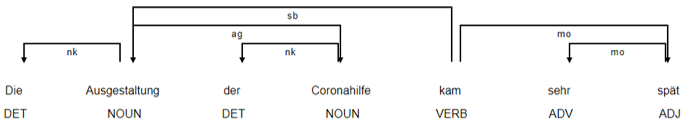
\includegraphics[width=1\textwidth]{chapters/04-Sentiment-Analyse/hessel.png}}
\caption{Beispielsatz mit Gradpartikel-Verstärkung (Zitat von Katja Hessel MdB, 206. Sitzung, 28.01.2021)}
\label{hessel}
\end{figure}

\subsection{Polaritätsberechnung}
\label{polberechnung}
Für die abschließende Berechnung der Polarität sind verschiedene Formeln denkbar. 
Sie sollten anhand von Textcharakteristika wie z.B. der Satz- oder Textlänge gewählt werden. 

Bei der Verwendung einer satzbasierten Polaritätsberechnung, bei welcher alle Polaritäten erst addiert und die Summe anschließend durch die Anzahl der Worte dividiert wird, kann ein unerwünschtes Phänomen auftreten: 
Längere Sätze erhaltenen ein stärker polarisiertes Ergebnis als vergleichbare kurze Sätze. 

Dies ist mit einer im Schnitt höheren Dichte an Worten mit Polaritäts-Wert in längeren Sätzen zu erklären. 
Um diesem Problem entgegen zu wirken, wurde in dieser Arbeit eine Min-Max-Skalierung (siehe Formeln 1 - 3) auf Dokumentebene implementiert \cite{g3_sentia}. 

Die Entscheidung, diese Normalisierung anhand der Länge des gesamten Textes durchzuführen, wurde aufgrund der Charakteristika der zu analysierenden Interaktionen getroffen. 
Denn diese bestehen zu einem überwiegenden Teil aus einem einzelnen Satz von jedoch sehr unterschiedlicher Länge. 

\begin{align}
p' &= \frac{ p + 1 }{ text.len + 1 } \text{ für p $>$ 0}\\
p' &= \frac{ p - 1 }{ text.len + 1 } \text{ für p $<$ 0}\\
p' &= p \text{ für p $=$ 0}
\end{align}

\section{Evaluierung}
\subsection{Sprache im Bundestag}
\label{sprachebundestag}
Während der Entwicklung dieser Arbeit und den regelmäßig angestellten Zwischentests wurde ersichtlich, dass sich die Sprache im Bundestag etwa von jener in sozialen Netzwerken oder Produktbewertungen unterschiedet. 
Ein Interaktionstext setzt sich sowohl aus einzelnen, langen und komplexe Sätze zusammen, als auch aus einzelnen Ausrufen wie \textit{\glqq eieiei!\grqq} zusammen. 

Aus diesem Grund wurde die in \ref{polberechnung} beschriebene Normalisierung verwendet, da herkömmliche Berechnungsformeln zunächst widersprüchliche Ergebnisse lieferten. 
Gleichzeitig verbesserte die manuelle Durchsicht der häufigsten 15.000 Worte und Anfertigung einer eigenen Bundestags-Wortliste das Ergebnis deutlich. 
Viele der regelmäßig in Bundestagssitzungen verwendeten Worte gehören zur \textit{Politik-Domäne} und treten deshalb nicht in den Quell-Wortlisten auf. 
Hier wird erwartet, dass eine noch umfangreichere Bundestags-Wortliste einen weiteren positiven Einfluss auf das Endergebnis hätte. 
Aus Zeit- sowie Kompetenzgründen wurde diese Liste jedoch nicht erweitert. 

\subsection{Ironie und Sarkasmus}
Ebenso wie die im vorherigen besprochene \textit{Politiksprache}, treten auch Ironie und Sarkasmus vermehrt in den Sitzungen des Bundestages auf. 
Einfach umrissen, handelt es sich dabei um ein Stilmittel, bei dem das Gegenteil vom Gesagten gemeint ist. 
Sarkasmus ist dabei eine verstärkte Form der Ironie und kann auch als ein Angriff verstanden werden. 

Selbst für den menschlichen Leser ist allein am geschriebenen Text nicht immer ersichtlich, ob eine Aussage ironisch gemeint ist. 
Vielmehr wird für die richtige Deutung die Stimmlage, Gestik und Mimik der sprechenden Person benötigt. 

Ironie und Sarkasmus könne also erst recht nicht mit dem in dieser Arbeit verwendeten Wortlisten-Ansatz erkannt werden, womit ein unbekannter Teil der Interaktionen im Ergebnis die falsche Polarität besitzt. 
Gleichwohl gibt es Ansätze aus dem Bereich des maschinellen Lernens, welche dieses Problem behandeln. 
Jedoch setzen diese einen entsprechend annotierten Korpus vorraus und stammen zudem aus dem Bereich der sozialen Netzwerke, in welchen etwa mit \textit{Hashtags} die Ironie bereits vom Autor markiert wurde. 

\subsection{Fazit}
Trotzt der soeben beschriebenen Fehlerquellen, wurde dennoch ein gelungenes Ergebnis erzielt: 
Es wurde ein solider und erweiterbarer Algorithmus zur Sentimentananlyse von Texten geschaffen, welcher auf den bekanntesten Bibliotheken und Techniken der Textverarbeitung beruht. 
Dieser kann als Basis für weitere Anstrengungen bei der Sentimentanalyse von politischen Texten dienen. 

Eine Deutung der bisherigen Ergebnisse durch Politikwissenschaftler oder anderweitig in diesem Bereich kompetente Personen wird dabei empfohlen, um die beschriebenen Schwachstellen entsprechend zu behandeln oder neue zu identifizieren. 

Der Programmcode ist zudem vollständig und abgesichert in die Projektpipeline eingebunden. 
Er erweitert seine Ergebnis-Datenbank automatisch um neue Sitzungen und benachrichtigt anschließend nachfolgende Gruppen. 

\section{Aufbau der Lösung}\label{sec:01_02_aufbauLoesung}
Das Projekt zur Entwicklung eines graphbasierten Informationssystem für die Analyse sozialer Interaktionen im Deutschen Bundestag, welches \glqq Sentiments Of Bundestag\grqq{} genannt wurde, besteht, wie bereits erwähnt, aus sieben Teilprojekten. Im folgenden Abschnitt wird grob auf die Thematiken der einzelnen Gruppen eingegangen.

\begin{figure}[H]
    \centering
    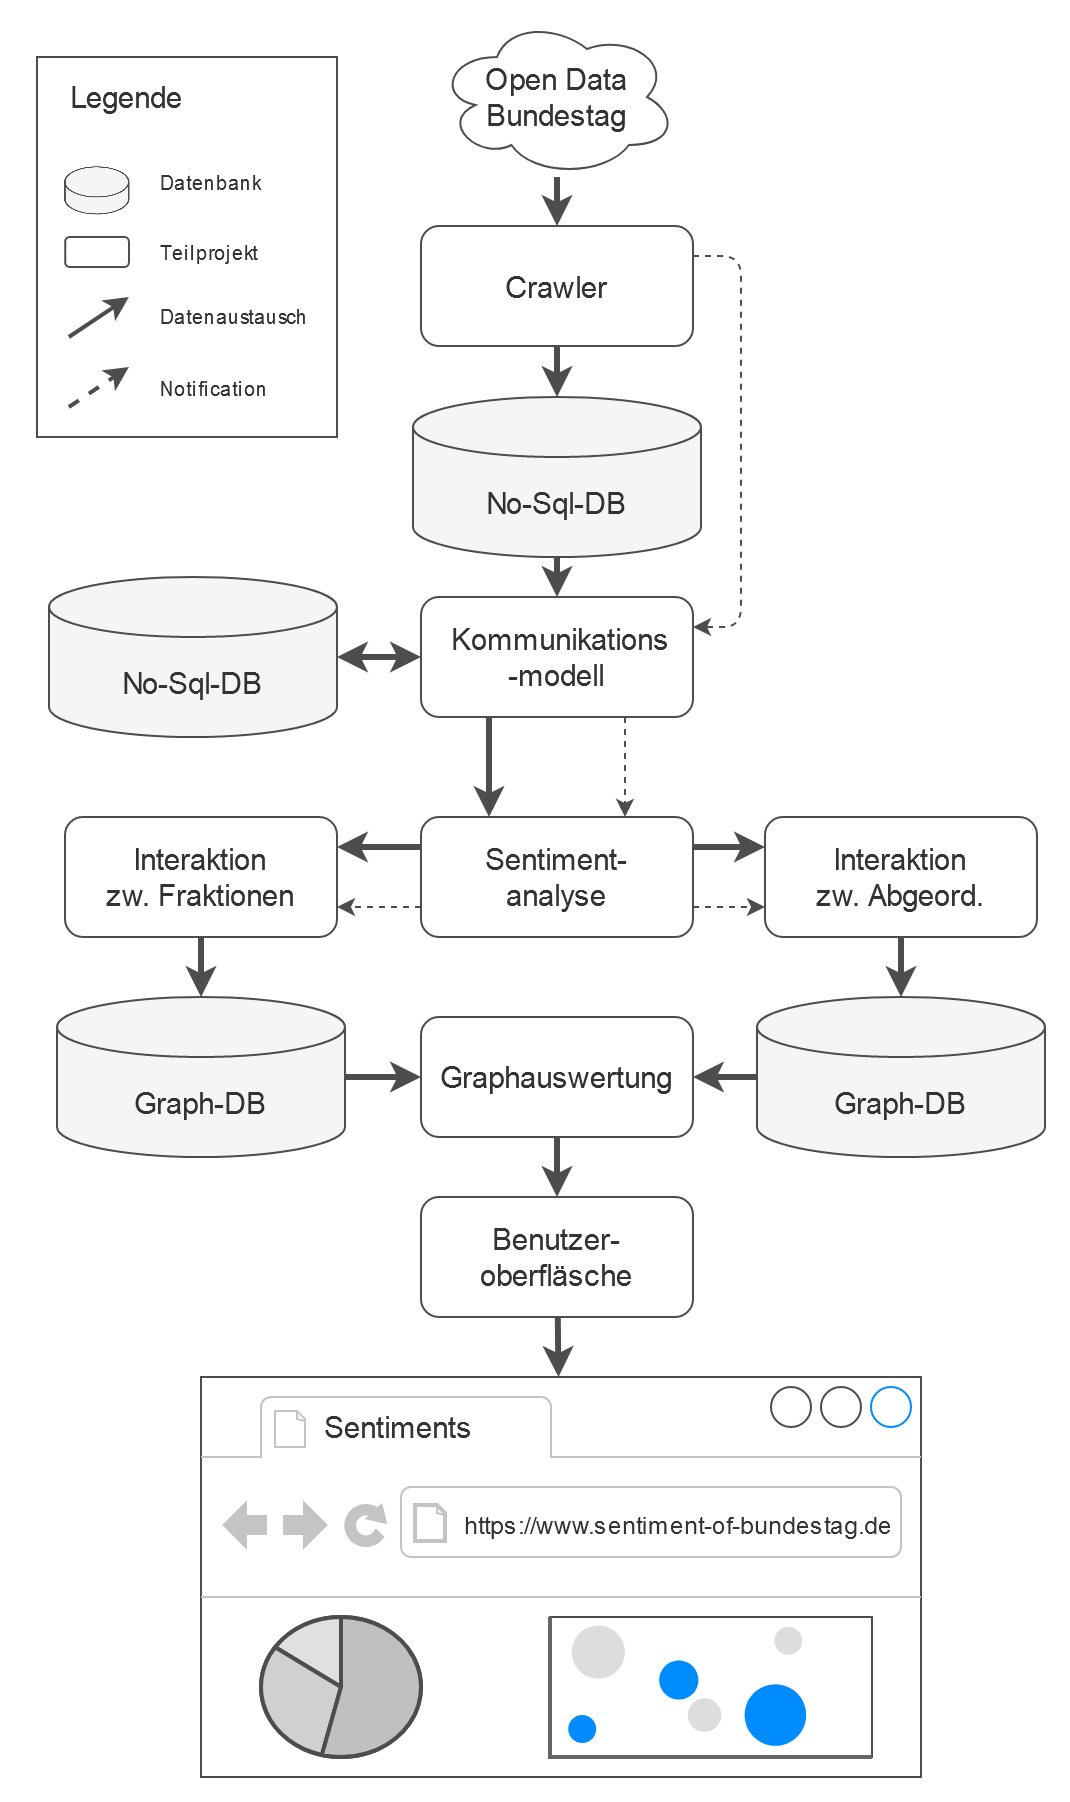
\includegraphics[width=\textwidth]{images/01-Einleitung/SentimentOfBundestag.png}
    \caption{Aufbau der Lösung}
    \label{fig:aufbauderLösungSOB}
\end{figure}

Die in der \autoref{fig:aufbauderLösungSOB} dargestellten Teilprojekte sind hier nun detaillierter aufgelistet:
\begin{itemize}
    \item \textbf{Crawler}: Scannt regelmäßig die Open Data Webseite des Bundestags, sucht, parst und speichern neue Protokollen sowie Stammdaten der Abgeordneten in seiner No-Sql-Datenbank. Ziel ist es hier sicherzustellen, das die DB immer auf dem neusten Stand bleibt
    \item \textbf{Kommunikationsmodell}: Analysiert und erstellt aus den
      Protokollen von Gruppe 1 ein Kommunikationsmodell, welches die möglichen
      Interaktionen im Bundestag abbildet
    \item \textbf{Sentiment-Analyse}: Sentiment Analysis (Stimmungsanalyse). Ziele sind hier die Identifikation der Stimmung in den Äußerungen der Abgeordneten und die Verrechnung der Stimmung einer Äußerung zu positiver/negativer Bewertung der Beziehung
    \item \textbf{Interaktion zwischen Abgeordneten}: Aus dem Kommunikationsmodell von Gruppe 2 und die Stimmungsanalyse von Gruppe 3 werden hier Interaktionen zwischen einzelnen Personen (Abgeordneten, Präsident, Gäste, etc.) identifiziert. Erstellt wird hier ein gewichteter Sentiment-Graph zwischen Abgeordneten mit positiven/negativen Gewichtungen
    \item \textbf{Interaktion zwischen Fraktionen}: Aus dem Kommunikationsmodell von Gruppe 2 und den Sentiment-Graph zwischen Personen von Gruppe 4 werden hier Interaktionen zwischen Gruppen von Personen analysiert und in einen Sentiment-Graph zwischen Parteien. Der besteht aus einer Aggregation der Abgeordnetensentiments zu gewichteten Sentiment-Graph der Parteien (Fraktionen, Gruppen, etc.)
    \item \textbf{Graphauswertung}: Die Sentiment-Graphen von den Gruppen 4 und 5 werden hier anhand verschiedener Auswertungsmethoden analysiert und die Ergebnisse davon die nächste Gruppe (Benutzeroberfläche) zur Verfügung stellt.
    \item \textbf{Benutzeroberfläche}: Ziel ist hier die Realisierung einer interaktiven Benutzeroberfläche zur Darstellung der ausgewerteten Ergebnisse
\end{itemize}

Die einzelnen Teilprojekte werden in den nächsten Kapiteln in dieser Reihenfolge näher erläutert.

\chapter{Crawler}
\thispagestyle{empty}
\begin{table}[ht]
\caption{Gruppe 1 (Crawler) - Arbeitsaufteilung}
\label{tab:zeittafelEU}
\centering
\begin{tabular}{m{12em}|m{12em}|m{8em}}
\hline
\rowcolor{Gray}
Aufgabe &Gruppenmietglieder &Anteil\\
\hline
\hline
\rowcolor{White}
Crawl-Manager& Boris Foko Kouti & ff\\
\hline
\hline
\rowcolor{White}
& Marlon Daniel Kohlberger & ff\\
\cline{2-3}
\rowcolor{White}
\multirow{-2}{*}{Crawl-Utilities}& Boris Foko Kouti & ff\\
\hline
\hline
\rowcolor{White}
& Marlon Daniel Kohlberger & ff\\
\cline{2-3}
\rowcolor{White}
\multirow{-2}{*}{DB-Manager}& Boris Foko Kouti & ff\\
\hline
\hline
\cline{2-3}
\rowcolor{White}
& Arnauld Feussi & ff\\
\rowcolor{White}
& Marlon Daniel Kohlberger & ff\\
\cline{2-3}
\rowcolor{White}
\multirow{-2}{*}{Dokumenation}& Boris Foko Kouti & ff\\
\hline
\hline
\rowcolor{White}
Bereitstellung der Lösung& Boris Foko Kouti & ff\\
\hline
\end{tabular}
\end{table}
\section{Einleitung}
Der Begriff \textit{Sentiment} stammt vom lateinischen Wort \textit{sentimentum} ab und bedeutet Empfindung oder Stimmung. 
In der Sentimentanalyse geht es um die Bestimmung eben jener Stimmung einer Meinungsäußerung. 
Anwendung findet sie etwa bei Produktbewertungen oder Beiträgen in sozialen Netzwerken. 
Die Stimmung wird durch die sog. Polarität beschrieben und kann positiv, negativ oder neutral ausfallen. 
Im Text-Mining wird sie im Intervall $\interval{-1}{1} = \{x \in \mathbb{R} | -1 \leq x \leq 1\}$ angegeben, wobei -1 sehr negativ, 1 sehr positiv und 0 neutral bedeuten. 

Grundlegend ist die maschinelle Sentimentanalyse entweder Wortlisten- oder Modell-basiert. 
Der Wortlisten-Ansatz kann als eine Sammlung von Worten und ihrer Polaritäten verstanden werden, anhand welcher die Stimmung berechnet wird. 
Dieser Ansatz wird weiter im Kapitel \ref{wortliste} beschrieben, da er in dieser Arbeit verwendet wurde. 

Bei der Modell-basierten Sentimentanalyse wird ein annotierter Satz-Korpus für das Trainieren einer künstlichen Intelligenz vorausgesetzt. 
Etwa für Twitter-Beiträge stehen solche Korpusse oder auch bereits trainierte Modelle zur Verfügung. 
Jedoch ist bei der Verwendung zur Analyse der Sitzungsprotokolle des Bundestages nicht mit zufriedenstellenden Ergebnissen zu rechnen, da sich verwendete Worte und Text- bzw. Satzbau zwischen diesen Domänen deutlich unterscheiden. 
Eine weitere Erläuterung zur Sprache im Bundestag wird in Kapitel \ref{sprachebundestag} gegeben. 

Ebenfalls werden die Komponenten zur Teilnahme an der Verarbeitungspipeline des Gesamtprojektes im nachfolgenden Kapitel \ref{g3daten} beschrieben. 

\section{Datenaustausch}
\label{g3daten}
\subsection{Datenimport}
Für das Erhalten von Daten wurde eine Methode implementiert, welche durch Angabe einer Sitzungs-ID die entsprechende Sitzung vom REST-API von Gruppe 2 abfragen kann. 
Diese Methode gibt jede Sitzung weiter an die in Kapitel \ref{g3textv} beschriebene Textverarbeitung und das Ergebnis schließlich an den in Kapitel \ref{g3export} beschriebenen Export-Code. 

Die Methode wird für zwei Fälle verwendet: 
Beim Normalfall sendet die Gruppe 2 eine Benachrichtigung mit einer Liste aller neuen Sitzungs-IDs an das REST-API im Code dieser Arbeit. 
Das REST-API wurde mit der Bibliothek \mintinline{latex}{Flask} \cite{g3_flask} entwickelt und besteht aus einer POST-Schnittstelle, welche auf dem von der HTW bereitgestelltem Server unter \textit{/notify} erreichbar ist. 

Das API wurde unter Zuhilfenahme von \mintinline{latex}{Flask.Blueprints} \cite{g3_flaskbp} entwickelt und wird von einem \mintinline{latex}{Waitress}-Webserver \cite{g3_waitress} bereitgestellt. 
Für jede Anfrage wird geprüft, ob Content-Type und Payload dem erwarteten JSON-Daten entsprechen. 
Sollte dies nicht der Fall sein, wird eine entsprechende Rückmeldung an den Sender zurückgegeben. 
Für jede erhaltene Sitzungs-ID wird die eingangs beschriebene Methode aufgerufen. 

Der zweite Fall wurde vor allem im Rahmen der voranschreitenden Entwicklung bei den in der Projektpipeline voranstehenden Gruppen verwendet. 
Statt auf eine Benachrichtigung zum Anstoßen des Datenimports zu warten, werden stattdessen alle Sitzungs-IDs vom REST-API der Gruppe 2 abgefragt und jede Sitzung vollständig neu importiert. 
Dieses Vorgehen hat den Vorteil, dass eventuell durch Arbeit am Code verpasste Benachrichtigungen nachgeholt werden und gleichzeitig Änderungen an den Daten übernommen werden können. 

\subsection{Datenexport}
\label{g3export}
Statt Arbeit in ein umfangreiches REST-API für die nachfolgenden Gruppen zu stecken, wurde für diese Arbeit ein reiner MongoDB-Ansatz verwendet. 
Auf dem zur Verfügung stehenden HTW-Server wurde dafür eine MongoDB Instanz aufgesetzt, welche nur aus dem HTW-Netz erreichbar und zudem nur mit Authentifizierung zugreifbar ist. 
Jede Sitzung ist hier als eine eigene Collection persistiert. 
Sobald neue Sitzungen importiert und verarbeitet wurden, werden diese zunächst mit dem MongoDB-Treiber \mintinline{latex}{PyMongo} \cite{g3_mongodb} in die Datenbank geschrieben. 
Anschließend werden die nachfolgenden Gruppen mit einem POST and die jeweilige REST-Schnittstelle benachrichtigt, dass neue Daten vorliegen. 
Diese greifen dann mit den zuvor versendeten Zugangsdaten direkt auf die Datenbank zu. 

Mit diesem Vorgehen konnte die Komplexität beim Zugriff auf die Ergebnis-Daten gesenkt werden, da es für nahezu alle gängigen Programmiersprachen einen intuitiven MongoDB-Treiber gibt. 

\section{Wortliste}
\label{wortliste}
Wie bereits in der Einleitung beschrieben, handelt es sich bei Wortlisten in der Sentimentanalyse um eine Liste von Worten und ihrer jeweiligen Polarität. 
Bei der Analyse eines Textes wird wortweise ein Abgleich mit dieser Liste durchgeführt und die Wort-Polarität bei einer Übereinstimmung für die Berechnung des Sentiments verwendet. 
Unterschiedliche Berechnungsformeln sind dabei denkbar und werden in Kapitel \ref{polberechnung} weiter besprochen. 
Für diese Arbeit wurden Wortlisten verschiedener Institutionen kombiniert und anschließend mit Synonymen erweitert. 
Ebenfalls wurde eine eigene Bundestags-Wortliste erstellt. 

Die Interest Group on German Sentiment Analysis (IGGSA) stellt eine umfangreiche Liste an Publikationen und Ressourcen zu Sentimentanalysen in der deutschen Sprache zur Verfügung \cite{g3_iggsa}. 
Hier wurden alle Referenzen auf die in dieser Arbeit verwendeten Quell-Wortlisten gesammelt. 
Für die Zusammenführung dieser Wortlisten wurden zunächst zwei Herangehensweisen evaluiert: 
Zum einen war die Erstellung eines eigenständigen Codes denkbar, welcher einmalig die Daten aus allen Quellen einliest, zusammenfasst und eine Ergebnis-Datei ausgibt. 
Diese Datei wäre eine Ressource für den eigentlichen Analyse-Code. 
Zum anderen könnte die soeben beschriebene Funktionalität jedoch auch direkt im Analyse-Code integriert und bei jedem Programmstart ausgeführt werden. 
Die kombinierte Wortliste würde somit nicht auf die Festplatte geschrieben, sondern im Arbeitsspeicher verbleiben, solange der Analyse-Code läuft. 
Wenngleich der zuerst beschriebene Ansatz offensichtlich weniger Rechenzeitaufwändig ist, wurde für diese Arbeit der zweite Ansatz gewählt. 
Dies wird vor allem mit Rechtsunsicherheiten bei der Arbeit mit den verschiedenen Lizenzen der Quelldateien begründet. 
Gleichzeitig arbeitet der Analyse-Code damit jederzeit mit dem aktuellen Stand der Quell-Wortlisten. 
Das Aufbauen der Wortliste dauert wenige Minuten. 

Für diese Arbeit wurden die folgenden Quell-Wortlisten verwendet: 

\begin{itemize}
\item \textit{SentimentWortschatz} (SentiWS) aus \glqq SentiWS - a Publicly Available German-language Resource for Sentiment Analysis\grqq (Universität Leipzig) \cite{g3_sentiws}
\item \textit{Multi-Domain Sentiment Lexicon for German} (Hochschule Darmstadt) \cite{g3_opm}
\item \textit{German Polarity Lexicon} aus \glqq Evaluation and extension of a polarity lexicon for German\grqq (Universität Zürich) \cite{g3_polcla}
\item \textit{morphcomp} aus \glqq Evaluating the morphological compositionality of pola-rity\grqq (Leibniz-Institut für Deutsche Sprache, Universität des Saarlandes) \cite{g3_morphcomp}
\end{itemize}

Aus diesen Quellen ergibt sich eine Wortliste mit etwa 14.000 einzigartigen Worten. 
Die Worte werden dabei mit der in Kapitel \ref{g3textv} beschriebenen Textverarbeitungspipeline lemmatisiert, also auf die Grundform zurückgeführt. 
Bei Überschneidungen wird ein Mittelwert über alle Polaritäts-Werte eines Wortes gebildet. 

Mithilfe des \textit{Open German WordNet} (OdeNet) \cite{g3_odenet} werden zu jedem Wort Synonyme gesammelt und ebenfalls der Wortliste hinzugefügt. 
Der Zugriff auf OdeNet geschieht dabei mit der python Bibliothek \mintinline{latex}{WN} \cite{g3_wn}. 
Die Verwendung dieser Bibliothek ist trivial, weshalb an dieser Stelle keine weitere Erläuterung gegeben wird. 
Die Wortliste wird durch das Hinzufügen von Synonymen um weitere rund 2.000 Worte erweitert. 

Wie bereits in der Einleitung erwähnt, wurde zudem eine eigene Bundes-tags-Wortliste erstellt. 
Hierzu wurden die 15.000 am häufigsten in den Sitzungsprotokollen vorkommenden Worte erfasst und analysiert. 
Dabei wurden jedoch nur jene Worte betrachtet, welche nicht bereits in der kombinierten Wortliste vorkommen. 
Ausgewählt wurden nur eindeutig positive oder negative Worte wie \textit{angemessen}, \textit{Bullshit}, \textit{Fehlentscheidung}, \textit{Milchmädchenrechnung}, \textit{Realitätsverweigerung}, \textit{Totalausfall} oder \textit{Verunglimpfung}. 
Insgesamt umfasst die Bundestags-Wortliste 217 Worte. 

Im Code wird der Zugriff auf die Wortliste mit der zentralen Klasse \mintinline{latex}{Lexicon} realisiert. 
Bei der Instanziierung der Klasse werden, wie im Vorherigen beschrieben, alle Wortlisten gesammelt, zusammengeführt und erweitert. 
Anschließend stellt die Klasse ein \mintinline{latex}{Dictionary} bereit, in welchem die Schlüssel die Worte und die Werte die Wort-Polarität angeben. 

\section{Textverarbeitung}
\label{g3textv}
Für die Textverarbeitung nutzt der Code dieser Arbeit vollständig die Funktionalitäten und Strukturen von \mintinline{latex}{spaCy} \cite{g3_spacy}. 
Die \mintinline{latex}{spaCy} Bibliothek stellt eine Textverarbeitungspipeline bereit, welche mithilfe eines vortrainierten Modells funktioniert. 
Für die deutsche Sprache wurde ein solches Modell mit dem TIGER Korpus der Universität Stuttgart trainiert. 
Der Korpus umfasst ca. 50.000 Sätze aus Texten der Frankfurter Rundschau. 
Die \mintinline{latex}{spaCy}-Pipeline besteht aus den folgenden Komponenten: 

\begin{itemize}
\item Tokenisierung (Text- und Satzzerteilung)
\item POS-Tagging (Wortartenerkennung)
\item Dependency-Parsing (Wortabhängigkeitenerkennung)
\item Lemmatisierung (Wortgrundformermittlung)
\item Entity-Recognition (Eigennamenerkennung)
\end{itemize}

Das Ergebnis der Pipeline ist ein \mintinline{latex}{Doc}-Objekt, welches das Ergebnis des gesamten in die Pipeline gegebenen Textes umfasst. 
Einzelne Sätze innerhalb des \mintinline{latex}{Doc}-Objektes werden mit \mintinline{latex}{Span}-Objekten beschrieben und einzelne Worte mit \mintinline{latex}{Token}-Objekten. 
Die Objekttypen besitzen jeweils eigene Methoden und Erweiterungsmöglichkeiten in Form von sog. \textit{extension attributes}. 

Sehr einfach und gleichzeitig umfangreich kann die \mintinline{latex}{spaCy}-Pipeline an die eigenen Bedürfnisse angepasst werden. 
So wurde die Berechnung des Sentiments eines Textes direkt an die Komponenten der Standart-Pipeline angehängt. 
Logisch unterteilt sich diese in die Komponenten:

\begin{itemize}
\item Negations-Erkennung (siehe \ref{neg-erkennung})
\item Verstärkungs-Erkennung (siehe \ref{ver-erkennung})
\item Polaritätsberechnung (siehe \ref{polberechnung})
\end{itemize}

Basis für das nachfolgende Kapitel \ref{neg-erkennung} ist dabei das Ergebnis des Depen-dency-Parsers von \mintinline{latex}{spaCy}. 
Dieser bestimmt die Abhängigkeiten zwischen den einzelnen Elementen eines Satzes. 
Diese Funktion gehört dem Themenbereich der Dependenzgrammatik an, in welcher gerichtete Beziehungen zwischen den Worten eines Satzes beschreibt werden. 
Ein Wort kann einen Vorgänger (Regent) und mehrere Nachfolger (Dependenten) besitzen. 
Die Gesamtheit der Beziehungen eines Satzes wird auch Abhängigkeitsbaum genannt. 

Zur Verdeutlichung soll die Abbildung \ref{steffi} dienen, welche mithilfe von \mintinline{latex}{spaCy.displaCy} erstellt wurde. 
Zu sehen ist hier der Abhängigkeitsbaum des Satzes \textit{\glqq Das ist doch fachlich Quatsch hoch sechs!\grqq}. 
An den gerichteten Kanten befindet sich die Angabe des Satzgliedes, unterhalb der Worte die Angabe der Wortart. 

\begin{figure}[htb]
\centerline{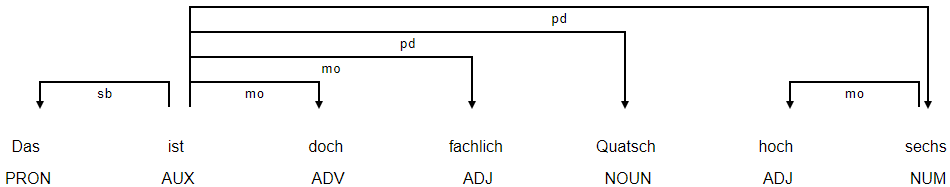
\includegraphics[width=1\textwidth]{chapters/04-Sentiment-Analyse/steffi.png}}
\caption{Visualisierung der Wortabhängigkeiten (Zitat von Steffi Lemke MdB, 208. Sitzung, 10.02.2021)}
\label{steffi}
\end{figure}

\subsection{Negations-Erkennung}
\label{neg-erkennung}
Negation, also Ablehnung, Verneinung oder Aufhebung, hat einen erheblichen Einfluss auf das Ergebnis und damit die Korrektheit der Sentimentanalyse, weshalb in dieser Arbeit ein besonderes Augenmerk auf ihre Erkennung gelegt wurde. 
In \textit{Negation Modeling for German Polarity Classification} \cite{g3_wieg} präsentieren Forscher der Universität des Saarlandes und des Leibniz-Institut für Deutsche Sprache hierfür einen regelbasierten Ansatz. 

Sie definieren unterschiedliche Negationstypen und ihre jeweilige Reichweite. 
So beeinflussen etwa negierende Adverbien oder Indefinitpronomen wie \textit{nie} den gesamten Satz, wohingegen das Partikel \textit{nicht} lediglich seinen Vorgänger negiert.  
Die Tabelle \ref{g3tab1} führt alle in dieser Arbeit implementierten Negationsregeln auf. 
Die Nutzung eines Abhängigkeitsbaumes, wie von \mintinline{latex}{spaCy} ermittelt, ist dabei unerlässlich. 
Denn wie schon im vorherigen Kapitel angesprochen, ist etwa mit dem Vorgänger eines Wortes nicht das in der Satzabfolge voranstehende Wort gemeint, sondern vielmehr der semantische Regent. 

\begin{table}[htbp]
\caption{Implementierte Negations-Regeln aus \cite{g3_wieg}}
\begin{center}
\begin{tabular}{| c | c | c |}
\hline
\textbf{Negationstyp} & \textbf{Reichweite} & \textbf{Beispielworte} \\ \hline
Partikel & Vorgänger (Regent) & nicht \\ \hline
Präpositionen & Nachfolger (Dependent) & ohne, gegen \\ \hline
Adverbien, & Satz & nie, kein, kaum \\
Indefinitpronomen &  &  \\ \hline
Nomen & Genitiv,& Abschaffung, \\
 & Präpositionalobjekt & Zerstörung \\ \hline
Verben & Objekt, Subjekt & enden, sinken, lindern \\
\hline
\end{tabular}
\label{g3tab1}
\end{center}
\end{table}

Angemerkt sei an dieser Stelle, dass es nicht möglich war, alle Regeln aus \cite{g3_wieg} zu implementieren, da der von den Forschern genutzte Dependency-Parser umfangreichere Ergebnisse liefert, als jener von \mintinline{latex}{spaCy}. 

Eine Liste mit Negationsworten und dem jeweiligen Negationstyp wurde \cite{g3_polcla} entnommen und ist ebenfalls über die Klasse \mintinline{latex}{Lexicon} zugreifbar. 
Die Klasse stellt ein \mintinline{latex}{Dictionary} bereit, in welchem die Schlüssel die Negationsworte und die Werte eine Liste der Reichweiten sind. 

Wenn in einem Text ein Negationswort auftritt, werden alle implementierten Regeln geprüft. 
Sollte es zu einem Treffer kommen, etwa wenn das Wort \textit{nicht} auftritt (siehe Abb. \ref{brandner}) und es einen Vorgänger gibt, werden alle Worte in Reichweite des Negationswortes negiert. 
Dies geschieht, indem für die jeweiligen Worte, welche wie in \ref{g3textv} beschrieben \mintinline{latex}{Token}-Objekte sind, ein eigenes Attribut mit der Bezeichnung \mintinline{latex}{negated} auf \mintinline{latex}{True} gesetzt wird. 
In der Polaritätsberechnung wird wortweise auf dieses Attribut geprüft und die Wort-Polarität bei einer Negierung mit -1 multipliziert. 

\begin{figure}[htb]
\centerline{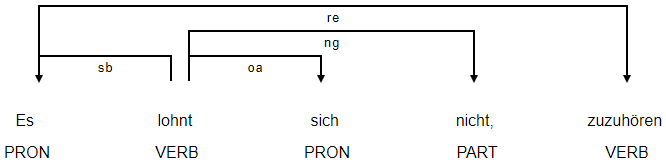
\includegraphics[width=1\textwidth]{chapters/04-Sentiment-Analyse/brandner.png}}
\caption{Beispielsatz mit Patikel-Negation (Zitat von Stephan Brandner MdB, 207. Sitzung, 29.01.2021)}
\label{brandner}
\end{figure}

\subsection{Verstärkungs-Erkennung}
\label{ver-erkennung}
Als \textit{Verstärker} werden sog. Gradpartikel (z.B. sehr, besonders, viel) verstanden, welche direkt vor Adjektiven oder Adverbien in einem Satz auftreten. 
Sie verstärken ihren Nachfolger, was wiederum in der Polaritätsberechnung berücksichtigt werden soll. 

Aus diesem Grund wird eine Liste mit verstärkenden Gradpartikeln, welche ebenfalls aus \cite{g3_polcla} bezogen werden, eingelesen und über die \mintinline{latex}{Lexicon} Klasse bereitgestellt. 

Ebenso wie in Kapitel \ref{neg-erkennung} bereits für die Negation beschrieben, wird ein eigenes Attribut zur Signalisierung einer Verstärkung definiert und im entsprechenden Fall auf True gesetzt. 
Bei der Polaritätsberechnung wird bei einer erkannten Verstärkung die Wort-Polarität mit 1,5 multipliziert \cite{g3_sentia}. 

In Abbildung \ref{hessel} wird ein Beispiel für das Auftreten eines verstärkenden Gradpartikels gegeben. 
Hier verstärkt das Wort \textit{sehr} das negative Wort \textit{spät}, womit die errechnete Polarität stärker negativ ausfällt als ohne die Verstärkungs-Erkennung. 

\begin{figure}[htb]
\centerline{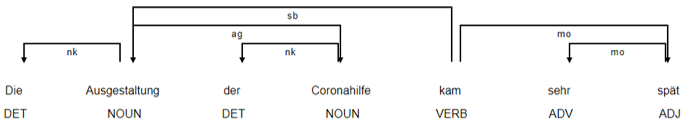
\includegraphics[width=1\textwidth]{chapters/04-Sentiment-Analyse/hessel.png}}
\caption{Beispielsatz mit Gradpartikel-Verstärkung (Zitat von Katja Hessel MdB, 206. Sitzung, 28.01.2021)}
\label{hessel}
\end{figure}

\subsection{Polaritätsberechnung}
\label{polberechnung}
Für die abschließende Berechnung der Polarität sind verschiedene Formeln denkbar. 
Sie sollten anhand von Textcharakteristika wie z.B. der Satz- oder Textlänge gewählt werden. 

Bei der Verwendung einer satzbasierten Polaritätsberechnung, bei welcher alle Polaritäten erst addiert und die Summe anschließend durch die Anzahl der Worte dividiert wird, kann ein unerwünschtes Phänomen auftreten: 
Längere Sätze erhaltenen ein stärker polarisiertes Ergebnis als vergleichbare kurze Sätze. 

Dies ist mit einer im Schnitt höheren Dichte an Worten mit Polaritäts-Wert in längeren Sätzen zu erklären. 
Um diesem Problem entgegen zu wirken, wurde in dieser Arbeit eine Min-Max-Skalierung (siehe Formeln 1 - 3) auf Dokumentebene implementiert \cite{g3_sentia}. 

Die Entscheidung, diese Normalisierung anhand der Länge des gesamten Textes durchzuführen, wurde aufgrund der Charakteristika der zu analysierenden Interaktionen getroffen. 
Denn diese bestehen zu einem überwiegenden Teil aus einem einzelnen Satz von jedoch sehr unterschiedlicher Länge. 

\begin{align}
p' &= \frac{ p + 1 }{ text.len + 1 } \text{ für p $>$ 0}\\
p' &= \frac{ p - 1 }{ text.len + 1 } \text{ für p $<$ 0}\\
p' &= p \text{ für p $=$ 0}
\end{align}

\section{Evaluierung}
\subsection{Sprache im Bundestag}
\label{sprachebundestag}
Während der Entwicklung dieser Arbeit und den regelmäßig angestellten Zwischentests wurde ersichtlich, dass sich die Sprache im Bundestag etwa von jener in sozialen Netzwerken oder Produktbewertungen unterschiedet. 
Ein Interaktionstext setzt sich sowohl aus einzelnen, langen und komplexe Sätze zusammen, als auch aus einzelnen Ausrufen wie \textit{\glqq eieiei!\grqq} zusammen. 

Aus diesem Grund wurde die in \ref{polberechnung} beschriebene Normalisierung verwendet, da herkömmliche Berechnungsformeln zunächst widersprüchliche Ergebnisse lieferten. 
Gleichzeitig verbesserte die manuelle Durchsicht der häufigsten 15.000 Worte und Anfertigung einer eigenen Bundestags-Wortliste das Ergebnis deutlich. 
Viele der regelmäßig in Bundestagssitzungen verwendeten Worte gehören zur \textit{Politik-Domäne} und treten deshalb nicht in den Quell-Wortlisten auf. 
Hier wird erwartet, dass eine noch umfangreichere Bundestags-Wortliste einen weiteren positiven Einfluss auf das Endergebnis hätte. 
Aus Zeit- sowie Kompetenzgründen wurde diese Liste jedoch nicht erweitert. 

\subsection{Ironie und Sarkasmus}
Ebenso wie die im vorherigen besprochene \textit{Politiksprache}, treten auch Ironie und Sarkasmus vermehrt in den Sitzungen des Bundestages auf. 
Einfach umrissen, handelt es sich dabei um ein Stilmittel, bei dem das Gegenteil vom Gesagten gemeint ist. 
Sarkasmus ist dabei eine verstärkte Form der Ironie und kann auch als ein Angriff verstanden werden. 

Selbst für den menschlichen Leser ist allein am geschriebenen Text nicht immer ersichtlich, ob eine Aussage ironisch gemeint ist. 
Vielmehr wird für die richtige Deutung die Stimmlage, Gestik und Mimik der sprechenden Person benötigt. 

Ironie und Sarkasmus könne also erst recht nicht mit dem in dieser Arbeit verwendeten Wortlisten-Ansatz erkannt werden, womit ein unbekannter Teil der Interaktionen im Ergebnis die falsche Polarität besitzt. 
Gleichwohl gibt es Ansätze aus dem Bereich des maschinellen Lernens, welche dieses Problem behandeln. 
Jedoch setzen diese einen entsprechend annotierten Korpus vorraus und stammen zudem aus dem Bereich der sozialen Netzwerke, in welchen etwa mit \textit{Hashtags} die Ironie bereits vom Autor markiert wurde. 

\subsection{Fazit}
Trotzt der soeben beschriebenen Fehlerquellen, wurde dennoch ein gelungenes Ergebnis erzielt: 
Es wurde ein solider und erweiterbarer Algorithmus zur Sentimentananlyse von Texten geschaffen, welcher auf den bekanntesten Bibliotheken und Techniken der Textverarbeitung beruht. 
Dieser kann als Basis für weitere Anstrengungen bei der Sentimentanalyse von politischen Texten dienen. 

Eine Deutung der bisherigen Ergebnisse durch Politikwissenschaftler oder anderweitig in diesem Bereich kompetente Personen wird dabei empfohlen, um die beschriebenen Schwachstellen entsprechend zu behandeln oder neue zu identifizieren. 

Der Programmcode ist zudem vollständig und abgesichert in die Projektpipeline eingebunden. 
Er erweitert seine Ergebnis-Datenbank automatisch um neue Sitzungen und benachrichtigt anschließend nachfolgende Gruppen. 

\section{Anforderungen und Rahmenbedingungen}\label{sec:02_02_anforderungen_rahmen}
Der zu entwickelnden Crawler soll in bestimmten Rahmenbedingungen einige Anforderungen erfüllen. Diese sowie die technischen und organisatorischen Rahmenbedingungen dazu werden in diesem Abschnitt aufgelistet. 
\subsection{Anforderungen an dem Crawler}\label{subsec:02_02_anforderungen}
Die Anforderungen an dem Crawler sind in~\cite{Hoppe2020Uebung} zusammengefasst und sehen vor, dass der Crawler kontinuierlich laufen sollte und dabei nach folgenden Dateien suchen:
\begin{itemize}
  \item \textbf{Protokolle}: Ein Protokoll ist eine XML-Datei, die den gesamten Ablauf einer Plenarsitzung (Inhaltsverzeichnis, Sitzungsverlauf mit Sitzungsbeginn, Tagesordnungspunkte, Sitzungsende, Anlagen, Rednerliste und  gewisse Konfigs) beinhaltet. Da sich die Formatierung der Protokollen in den Jahren stets verbessert hat, soll hier auf die Legislaturperioden geachtet werden:
  \begin{itemize}
    \item 19. Legislaturperiode: diese sind sehr gut strukturiert und leicht zu parsen
    \item 18. Legislaturperiode: schlechter formatiert als die 19. Legislaturperiode. Hierfür wird vom Prof. Dr. Thomas Hoppe eine mit besser formatierte Version zur Verfügung gestellt
  \end{itemize}
  \item \textbf{Stammdaten der Abgeordneten}: Ist eine XML-Datei, die Informationen über Abgeordneten seit 1949 sammelt
  \item \textit{Optional} \textbf{Namentliche Abstimmungen}: Liste aller namentlichen Abstimmungen im Bundestag seit dem 18.12.2009 in PDF-Format und seit dem 18.10.2012 auch in XLSX-Format~\cite{NamentlicheAbstimmung20}
  \item Es muss sichergestellt sein, dass alle Daten immer auf dem neusten Stand sind. Dafür soll die Frequenz des Crawlers sich an dem Sitzungskalender des Bundestags~\cite{Sitzungskalender2021} orientieren
\end{itemize}

\subsection{Rahmenbedingungen}\label{subsec:02_02_rahmenbedingungen}
\subsubsection{Organisatorische Rahmenbedingungen}
Für die Planung des gesamten Projekts ist in einem zwei Wochen-Takt ein Plenum für den Brainstorming und eventuelle Teams-übergreifende Abstimmungen festgelegt worden. Im Team-Crawler (Gruppe 1) ist folgende Planung abgemacht worden:
\begin{itemize}
    \item Ziel bis zum 13.11.2020: Testdaten für andere Gruppen, erster lauffähiger Prototyp
    \item Ziel bis zum 27.11.2020: Vorläufiger Release und Integration-Test mit anderen Gruppen (Kommunikationsmodell)
    \item Ziel bis zum 04.12.2020: finale Version und Anfang der Dokumentation
    \item Ziel bis zum 25.02.2021: Fertigstellung der Dokumentation und Abgabe
\end{itemize}
Neben den organisatorischen Rahmenbedingungen sind technische Rahmenbedingungen zu betrachten bzw. sind Fehler (Probleme) zu vermeiden (zu lösen).
\subsubsection{Technische Rahmenbedingungen: Probleme beim Crawlen}\label{subsubsec:techAnforderungen}
\begin{itemize}
    \item Sperrung durch Server-Administrator (Server-Regel). Es soll vermieden werden, dass der ausführende Rechner wegen zu häufige Abfragen vom Server-Admin gesperrt wird und nur noch ein 500-Fehlercode erhält
    \item Ajax basierende Inhalte. Die Open Data Webseite verwendet Ajax für die Bereitstellung der Daten und lädt diese im Hintergrund. Ein einfacher Download der Seite genug da nicht. Außerdem nutzen die meisten Links, hinter denen Dateien stehen, Javascript (es ist z. B. der Fall bei Slides und verborgenen Regionen). Dies muss entsprechend gehandelt werden
    \item Mongo-DB-Konfiguration und Zurverfügungstellung der Daten für die Gruppe Kommunikationsmodell 
    %\item Das robots.txt Protokoll
\end{itemize}
\section{Lösung und Konzepte}\label{sec:02_03_loesung_konzept}
\subsection{Standard Aufbau eines Crawlers}
\begin{wrapfigure}{R}{0.4\textwidth}
  \centering
    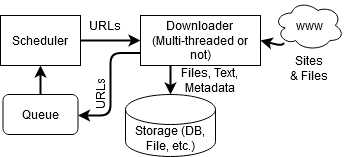
\includegraphics[width=0.4\textwidth]{images/02-Crawler/Crawler-Standard-Crawler.png}
  \caption{\label{fig:standardCrawler}Crawler: Standard Aufbau}
\end{wrapfigure}
Ein Crawler besteht in der Regel aus zwei wichtigen Teilen: ein Downloader und ein Scheduler. Der Downloader ist mit dem Webserver verbunden und lädt die Webseite(n) sowie alle erwünschten Dateien herunter. Der Scheduler ist, wie der Name schon sagt, für die Planung zuständig und erteilt dem Downloader URLs nach internen Priorisierung-Mechanismen (als Liste FIFO und als Graph mit DFS und BFS ~\cite{ThomasAlgorithms2009}--\cite{DonaldKnuth1998}). 
\subsection{Crawler Mechanismus}
Für unseren speziellen Fall, wird die Aufgaben von dem Scheduler vom Crawl-Manager übernommen, der sowohl für die Planung als auch für die Steuerung (Start, Pause, Stopp, Zustand) laufender Crawl-Aufgaben zuständig ist. Der Crawl-Manager erzeugt für jede URL ein Thread (Page-Crawler), dessen Aufgabe darin besteht die Seite herunterzuladen, mit seinem Page-Analyser nach relevanten Inhalten in der Seite zu suchen (URLs, Dateien, Action-Links: Javascript, etc.) und bei Bedarf weitere parallele Sub-Threads für den Download, das Parsen und die Speicherung der relevanten Dateiinhalte (Protokollen, Stammdaten, weitere Metadaten). Dieser Mechanismus wird durch die Abb.~\ref{fig:funktionsprinzipCrawler} und die Abb.~\ref{fig:crawlEinerUrl} veranschaulicht.

\begin{figure}[H]
    \centering
    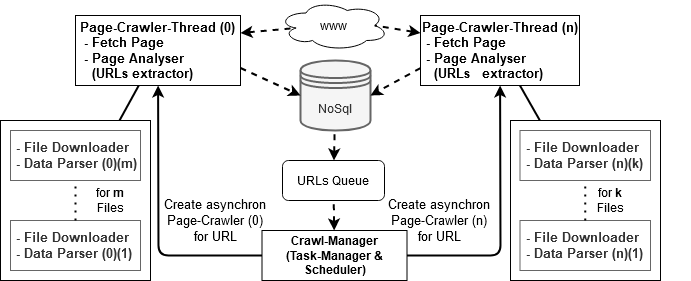
\includegraphics[width=5in]{images/02-Crawler/Crawler-Process-Diagram (Multithreading).png}
    \caption{Funktionsprinzip des unseres Crawlers}
    \label{fig:funktionsprinzipCrawler}
\end{figure}

\begin{figure}[H]
    \centering
    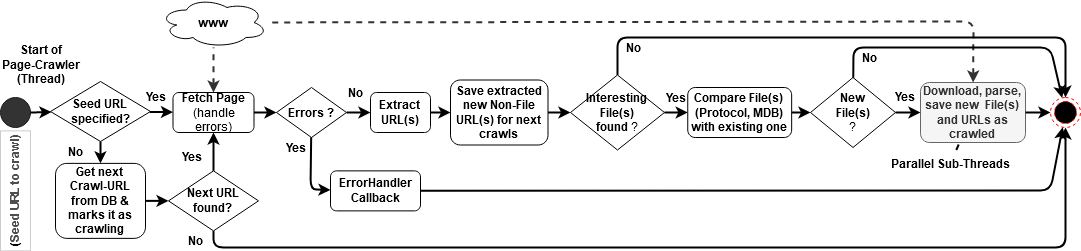
\includegraphics[width=5.5in]{images/02-Crawler/Crawler-Process-Diagram (Page-Crawler).png}
    \caption{Page-Crawler für eine URL}
    \label{fig:crawlEinerUrl}
\end{figure}
\noindent
Ein Crawl auf einer Seite (durch den Page-Crawl) kann in einer durch den Scheduler (Crawl-Manager) regelmäßig gemacht werden, in dem dieser nach einer bestimmten Zeit einen neuen Page-Crawl-Thread startet. Die Frequenz der Generierung dieses Threads orientiert sich an dem Sitzungskalender des Bundestags~\cite{Sitzungskalender2021}. Dieser Kalender sieht vor, dass Sitzungen an bestimmten Wochentagen zwei bis vier Wochen pro Monat (abgesehen von August: Ferien) stattfinden. Darauf basierend ist die Entscheidung getroffen worden, die Frequenz auf einmal pro Tag von Montag bis Freitag (mit der Möglichkeit bei Bedarf den Crawler in der Ferienzeit zu stoppen) festzulegen. So lässt sich eine Sperrung wegen zu häufiger Abfragen verhindern. Bei Manchen Server (durch Regeln oder Server-Admin) kann aber ein sich wiederholender Abfrage-Muster (wie eine Abfrage jeden Tag um dieselbe Uhrzeit) auch zu einer Sperrung der IP (Rechner) führen. Aus diesem Grund wird zusätzlich zur Frequenz ein Zufallsfaktor verwendet. Ein Page-Crawl-Thread wird zwar von Montag bis Freitag um 23Uhr durch den Crawl-Manager gestartet, allerdings wartet dieser Thread ein zufällige Zeit $t$ (mit $10 \leq t \leq 7200 $) bis er den tatsächlichen Crawl durchführt. Während und nach dem Crawl-Prozess werden Daten (und Dateien) manipuliert, analysiert und gespeichert. Diese Vorgänge sowie die dafür verwendeten Datenstrukturen werden im nächsten Abschnitt beleuchtet. 

\subsection{Daten-Parser und Database-Modell}
- Parser für die 19. Legislaturperiode\\
- Parser für die 18. Legislaturperiode\\
- ER-Diagramm und Beschreibung des DB-Modells

\subsection{Gesamter Aufbau der Lösung}
Die gesamte Lösung besteht aus vier Komponenten und einer Datenbank, wie auf die Abb.~\ref{fig:crawlerKompoenenten} dargestellt. 
\begin{itemize}
    \item \textbf{Crawl-Manager}: Taskmanager und Scheduler
    \item \textbf{Crawl-Utilities}: Liefert die für den Crawl-Prozess nötigen Funktionalitäten (Page-Fetcher, Page-Analyser, Downloader, Data-Parser)
    \item \textbf{DB-Manager}: Verwaltet den Zugriff auf die Datenbank 
    \item \textbf{Rest-ServiceProvider}: Rest-API für die Steuerung des Crawl-Manager und den eingeschränkten Zugriff auf die DB-Daten
    \item \textbf{Datenbank}: NoSql (MongoDB) Datenbank für die Sicherung der Daten
\end{itemize}

\begin{figure}[H]
    \centering
    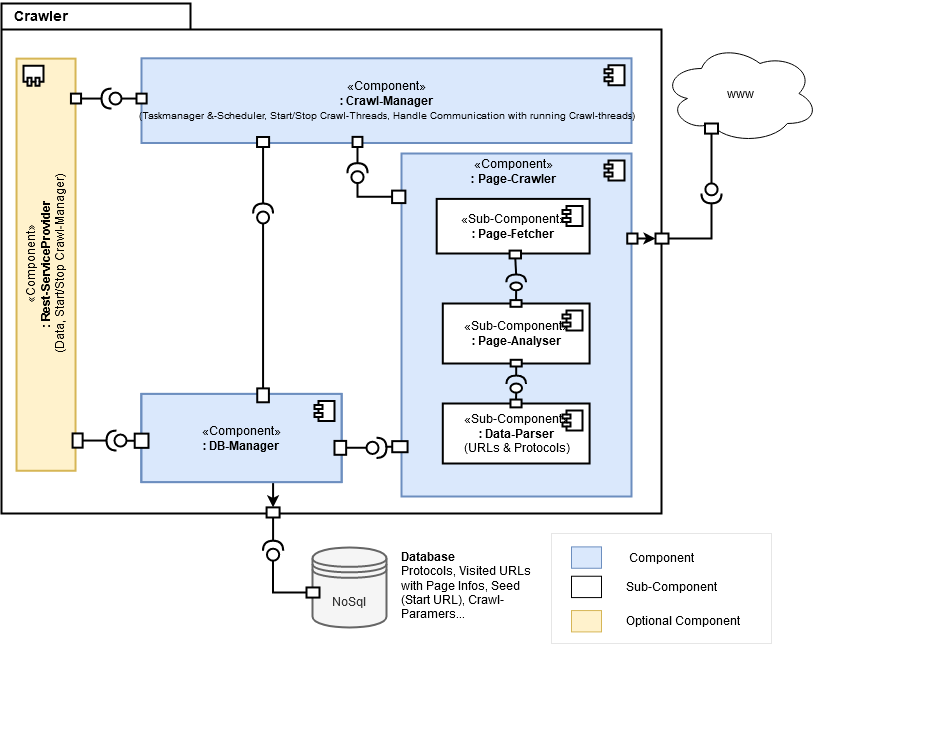
\includegraphics[width=5in]{images/02-Crawler/Crawler-Component-Diagram.png}
    \caption{Crawler: Komponentendiagramm}
    \label{fig:crawlerKompoenenten}
\end{figure}
\noindent
Am Ende eines Crawl-Prozess, bei dem neue Protokolle oder Stammdaten geladen worden sind, wird die Gruppe-Kommunikationsmodell die Liste aller Protokollen sowie Stammdaten über deren Rest-API~\cite{Cme2021} als Json-Datei mitgeteilt. Die Gruppe-Kommunikationsmodell kann dann asynchron die entsprechenden Dateien aus unseren Datenbank holen.
\section{Implementierung und Bereitstellung der Lösung}\label{sec:02_04_implementierung_bereitstellung}

\subsection{Implementierung des Crawlers}
Für die Umsetzung des Crawler wurde die Entscheidung getroffen eine Web-Anwendung (Rest-Schnittstelle, Crawl-Prozess und Scheduler) zu bauen. Dafür wurde Spring Boot~\cite{SpringBoot242} als Java-basierender Framework für die Entwicklung von Web-Anwendungen gewählt. Damit lassen sich Konfigurationen (für Rest-APIs, Datenbanktreiber, etc.) mit Hilfe des Spring-Initializers vereinfachen. Außerdem verfügt Spring Boot über einen eigenen Task-Scheduler der für den Crawl-Manager verwendet werden kann. Die finale Lösung beinhaltet vier Packages: \textbf{crawler} mit den Funktionalitäten für den Crawl-Prozess und das Parsen, \textbf{models} und \textbf{repositories} für den DB-Manager und \textbf{web} mit den Controllers für die Rest-Schnittstelle und den Services für den Crawl-Manager. Das gesamte Projekt-Verzeichnis inkl. Code ist auf dem Github-Repository \textit{Sentiments-of-Bundestag/Crawler}~\cite{Crawler2021} zu finden. Dort kommt unter anderem für die Ausführung Javascript-basierende Inhalte für den Download bestimmter Teile (Protokoll-Slides) der Webseite die \\\textbf{HtmlUnit}-Bibliothek~\cite{HtmlUnit2021} zum Einsatz (siehe ~\ref{subsubsec:techAnforderungen}).

\subsection{Bereitstellung der Lösung}
Der Crawler wurde auf dem Virtual-Server der Gruppe 1 (141.45.146.161) an der HTW (nur im HTW-Netz sichtbar) als Ubuntu-Service bereitgestellt. Der Crawler-Service liefert eine Rest-Schnittstelle, die jedoch nur auf dem infosys1 Rechner aus Sicherheitsgründen zugänglich ist. Die Konfiguration des Crawler-Services, die unter \textit{/etc/systemd/system/crawler.service} angelegt wird, sieht wie folgt aus (Start des Crawlers: systemctl enable crawler):
\begin{lstlisting}
[Unit]
Description=Crawler App
...
User=local
[Service]
ExecStart=/usr/bin/java -jar ../Crawler-1.0-SNAPSHOT.jar
Restart=always
SyslogIdentifier=crawler
...
[Install]
WantedBy=multi-user.target
\end{lstlisting}
Da für den Crawler eine MongoDB benötigt wird, soll diese auch bei der Bereitstellung konfiguriert werden. Dabei muss sichergestellt werden, dass der zugriff auf die Datenbank nur mit den entsprechenden Zugangsdaten erfolgt. Also soll nach dem Hinzufügen eines neuen Admin-User die Security-Konfiguration von mongod unter \textit{sudo nano /etc/mongod.conf} auf \textit{authorization: enabled} umgestellt werden. Da die MongoDB von der Gruppe 2 (Kommunikationsmodell) verwendet wird, sollen dafür entsprechend die Firewall-Regeln angepasst werden. Der nachfolgende Auszug aus unserer Konfiguration-Datei (/root/Firewall.sh) zeigt wie dies beispielhaft erfolgen sollte.
\begin{lstlisting}
...
#
# Erlaube zugang im 145.45.x.x port 27017 MongoDB
#
iptables -A INPUT -s 141.45.0.0/16 -p tcp -m tcp --dport 27017 -j ACCEPT
...
\end{lstlisting}

Der bereitgestellten Crawler basiert auf Java 11 und ist somit eine Plattform-unabhängige Lösung, die auf allen Betriebssystemen angeboten werden kann. Die Steuerung des Crawlers erfolgt ausschließlich über die Rest-Schnittstelle mit folgenden Abfragen (hier mit curl in der Shell-Konsole):
\begin{lstlisting}
# opendata: https://www.bundestag.de/services/opendata
# Start a default crawl to opendata
$ curl -X POST http://localhost:8080/task/default
# Start the default cron process to opendata: Mon - Fri, 23
$ curl -X POST http://localhost:8080/task/cron
# List all running tasks
$ curl -X GET http://localhost:8080/tasks 
# Cancel planed task
$ curl -X POST http://localhost:8080/task/cancel/{task_id}
# Cancel all planed tasks
$ curl -X POST http://localhost:8080/tasks/cancel
\end{lstlisting}

Der Crawler auf dem infosys1-Server (infosys1.f4.htw-berlin.de) läuft seit dem 27.11.2020 mit ein Paar Unterbrechungen für Aktualisierungen problemlos und konnte zum Zeitpunkt der Verfassung dieser Dokumentation schon 204 Protokollen herunterladen, parsen und in der MongoDB speichern, Stammdaten von 4.086 Abgeordneten sammeln und dabei mehr als 500 Urls durchsuchen. Was den Datenaustausch mit anderen Gruppen angeht, konnte bis jetzt erfolgreich durch Gruppe 2 auf unsere MongoDB zugegriffen werden und Mitteilungen von neu gecrawlten Daten konnten fehlerfrei zugestellt werden.\\
Aus den vom Crawler gesammelten Daten wird nun durch Gruppe 2 ein Kommunikationsmodell gebaut, das von den anderen Gruppen für weitere Verarbeitungen und Analysen verwendet wird. Der Aufbau dieses Kommunikationsmodells wird nun von Gruppe 2 im nächsten Kapitel aufgegriffen. 

\chapter{Kommunikationsmodell}
\section{Einleitung}
Der Begriff \textit{Sentiment} stammt vom lateinischen Wort \textit{sentimentum} ab und bedeutet Empfindung oder Stimmung. 
In der Sentimentanalyse geht es um die Bestimmung eben jener Stimmung einer Meinungsäußerung. 
Anwendung findet sie etwa bei Produktbewertungen oder Beiträgen in sozialen Netzwerken. 
Die Stimmung wird durch die sog. Polarität beschrieben und kann positiv, negativ oder neutral ausfallen. 
Im Text-Mining wird sie im Intervall $\interval{-1}{1} = \{x \in \mathbb{R} | -1 \leq x \leq 1\}$ angegeben, wobei -1 sehr negativ, 1 sehr positiv und 0 neutral bedeuten. 

Grundlegend ist die maschinelle Sentimentanalyse entweder Wortlisten- oder Modell-basiert. 
Der Wortlisten-Ansatz kann als eine Sammlung von Worten und ihrer Polaritäten verstanden werden, anhand welcher die Stimmung berechnet wird. 
Dieser Ansatz wird weiter im Kapitel \ref{wortliste} beschrieben, da er in dieser Arbeit verwendet wurde. 

Bei der Modell-basierten Sentimentanalyse wird ein annotierter Satz-Korpus für das Trainieren einer künstlichen Intelligenz vorausgesetzt. 
Etwa für Twitter-Beiträge stehen solche Korpusse oder auch bereits trainierte Modelle zur Verfügung. 
Jedoch ist bei der Verwendung zur Analyse der Sitzungsprotokolle des Bundestages nicht mit zufriedenstellenden Ergebnissen zu rechnen, da sich verwendete Worte und Text- bzw. Satzbau zwischen diesen Domänen deutlich unterscheiden. 
Eine weitere Erläuterung zur Sprache im Bundestag wird in Kapitel \ref{sprachebundestag} gegeben. 

Ebenfalls werden die Komponenten zur Teilnahme an der Verarbeitungspipeline des Gesamtprojektes im nachfolgenden Kapitel \ref{g3daten} beschrieben. 

\section{Datenaustausch}
\label{g3daten}
\subsection{Datenimport}
Für das Erhalten von Daten wurde eine Methode implementiert, welche durch Angabe einer Sitzungs-ID die entsprechende Sitzung vom REST-API von Gruppe 2 abfragen kann. 
Diese Methode gibt jede Sitzung weiter an die in Kapitel \ref{g3textv} beschriebene Textverarbeitung und das Ergebnis schließlich an den in Kapitel \ref{g3export} beschriebenen Export-Code. 

Die Methode wird für zwei Fälle verwendet: 
Beim Normalfall sendet die Gruppe 2 eine Benachrichtigung mit einer Liste aller neuen Sitzungs-IDs an das REST-API im Code dieser Arbeit. 
Das REST-API wurde mit der Bibliothek \mintinline{latex}{Flask} \cite{g3_flask} entwickelt und besteht aus einer POST-Schnittstelle, welche auf dem von der HTW bereitgestelltem Server unter \textit{/notify} erreichbar ist. 

Das API wurde unter Zuhilfenahme von \mintinline{latex}{Flask.Blueprints} \cite{g3_flaskbp} entwickelt und wird von einem \mintinline{latex}{Waitress}-Webserver \cite{g3_waitress} bereitgestellt. 
Für jede Anfrage wird geprüft, ob Content-Type und Payload dem erwarteten JSON-Daten entsprechen. 
Sollte dies nicht der Fall sein, wird eine entsprechende Rückmeldung an den Sender zurückgegeben. 
Für jede erhaltene Sitzungs-ID wird die eingangs beschriebene Methode aufgerufen. 

Der zweite Fall wurde vor allem im Rahmen der voranschreitenden Entwicklung bei den in der Projektpipeline voranstehenden Gruppen verwendet. 
Statt auf eine Benachrichtigung zum Anstoßen des Datenimports zu warten, werden stattdessen alle Sitzungs-IDs vom REST-API der Gruppe 2 abgefragt und jede Sitzung vollständig neu importiert. 
Dieses Vorgehen hat den Vorteil, dass eventuell durch Arbeit am Code verpasste Benachrichtigungen nachgeholt werden und gleichzeitig Änderungen an den Daten übernommen werden können. 

\subsection{Datenexport}
\label{g3export}
Statt Arbeit in ein umfangreiches REST-API für die nachfolgenden Gruppen zu stecken, wurde für diese Arbeit ein reiner MongoDB-Ansatz verwendet. 
Auf dem zur Verfügung stehenden HTW-Server wurde dafür eine MongoDB Instanz aufgesetzt, welche nur aus dem HTW-Netz erreichbar und zudem nur mit Authentifizierung zugreifbar ist. 
Jede Sitzung ist hier als eine eigene Collection persistiert. 
Sobald neue Sitzungen importiert und verarbeitet wurden, werden diese zunächst mit dem MongoDB-Treiber \mintinline{latex}{PyMongo} \cite{g3_mongodb} in die Datenbank geschrieben. 
Anschließend werden die nachfolgenden Gruppen mit einem POST and die jeweilige REST-Schnittstelle benachrichtigt, dass neue Daten vorliegen. 
Diese greifen dann mit den zuvor versendeten Zugangsdaten direkt auf die Datenbank zu. 

Mit diesem Vorgehen konnte die Komplexität beim Zugriff auf die Ergebnis-Daten gesenkt werden, da es für nahezu alle gängigen Programmiersprachen einen intuitiven MongoDB-Treiber gibt. 

\section{Wortliste}
\label{wortliste}
Wie bereits in der Einleitung beschrieben, handelt es sich bei Wortlisten in der Sentimentanalyse um eine Liste von Worten und ihrer jeweiligen Polarität. 
Bei der Analyse eines Textes wird wortweise ein Abgleich mit dieser Liste durchgeführt und die Wort-Polarität bei einer Übereinstimmung für die Berechnung des Sentiments verwendet. 
Unterschiedliche Berechnungsformeln sind dabei denkbar und werden in Kapitel \ref{polberechnung} weiter besprochen. 
Für diese Arbeit wurden Wortlisten verschiedener Institutionen kombiniert und anschließend mit Synonymen erweitert. 
Ebenfalls wurde eine eigene Bundestags-Wortliste erstellt. 

Die Interest Group on German Sentiment Analysis (IGGSA) stellt eine umfangreiche Liste an Publikationen und Ressourcen zu Sentimentanalysen in der deutschen Sprache zur Verfügung \cite{g3_iggsa}. 
Hier wurden alle Referenzen auf die in dieser Arbeit verwendeten Quell-Wortlisten gesammelt. 
Für die Zusammenführung dieser Wortlisten wurden zunächst zwei Herangehensweisen evaluiert: 
Zum einen war die Erstellung eines eigenständigen Codes denkbar, welcher einmalig die Daten aus allen Quellen einliest, zusammenfasst und eine Ergebnis-Datei ausgibt. 
Diese Datei wäre eine Ressource für den eigentlichen Analyse-Code. 
Zum anderen könnte die soeben beschriebene Funktionalität jedoch auch direkt im Analyse-Code integriert und bei jedem Programmstart ausgeführt werden. 
Die kombinierte Wortliste würde somit nicht auf die Festplatte geschrieben, sondern im Arbeitsspeicher verbleiben, solange der Analyse-Code läuft. 
Wenngleich der zuerst beschriebene Ansatz offensichtlich weniger Rechenzeitaufwändig ist, wurde für diese Arbeit der zweite Ansatz gewählt. 
Dies wird vor allem mit Rechtsunsicherheiten bei der Arbeit mit den verschiedenen Lizenzen der Quelldateien begründet. 
Gleichzeitig arbeitet der Analyse-Code damit jederzeit mit dem aktuellen Stand der Quell-Wortlisten. 
Das Aufbauen der Wortliste dauert wenige Minuten. 

Für diese Arbeit wurden die folgenden Quell-Wortlisten verwendet: 

\begin{itemize}
\item \textit{SentimentWortschatz} (SentiWS) aus \glqq SentiWS - a Publicly Available German-language Resource for Sentiment Analysis\grqq (Universität Leipzig) \cite{g3_sentiws}
\item \textit{Multi-Domain Sentiment Lexicon for German} (Hochschule Darmstadt) \cite{g3_opm}
\item \textit{German Polarity Lexicon} aus \glqq Evaluation and extension of a polarity lexicon for German\grqq (Universität Zürich) \cite{g3_polcla}
\item \textit{morphcomp} aus \glqq Evaluating the morphological compositionality of pola-rity\grqq (Leibniz-Institut für Deutsche Sprache, Universität des Saarlandes) \cite{g3_morphcomp}
\end{itemize}

Aus diesen Quellen ergibt sich eine Wortliste mit etwa 14.000 einzigartigen Worten. 
Die Worte werden dabei mit der in Kapitel \ref{g3textv} beschriebenen Textverarbeitungspipeline lemmatisiert, also auf die Grundform zurückgeführt. 
Bei Überschneidungen wird ein Mittelwert über alle Polaritäts-Werte eines Wortes gebildet. 

Mithilfe des \textit{Open German WordNet} (OdeNet) \cite{g3_odenet} werden zu jedem Wort Synonyme gesammelt und ebenfalls der Wortliste hinzugefügt. 
Der Zugriff auf OdeNet geschieht dabei mit der python Bibliothek \mintinline{latex}{WN} \cite{g3_wn}. 
Die Verwendung dieser Bibliothek ist trivial, weshalb an dieser Stelle keine weitere Erläuterung gegeben wird. 
Die Wortliste wird durch das Hinzufügen von Synonymen um weitere rund 2.000 Worte erweitert. 

Wie bereits in der Einleitung erwähnt, wurde zudem eine eigene Bundes-tags-Wortliste erstellt. 
Hierzu wurden die 15.000 am häufigsten in den Sitzungsprotokollen vorkommenden Worte erfasst und analysiert. 
Dabei wurden jedoch nur jene Worte betrachtet, welche nicht bereits in der kombinierten Wortliste vorkommen. 
Ausgewählt wurden nur eindeutig positive oder negative Worte wie \textit{angemessen}, \textit{Bullshit}, \textit{Fehlentscheidung}, \textit{Milchmädchenrechnung}, \textit{Realitätsverweigerung}, \textit{Totalausfall} oder \textit{Verunglimpfung}. 
Insgesamt umfasst die Bundestags-Wortliste 217 Worte. 

Im Code wird der Zugriff auf die Wortliste mit der zentralen Klasse \mintinline{latex}{Lexicon} realisiert. 
Bei der Instanziierung der Klasse werden, wie im Vorherigen beschrieben, alle Wortlisten gesammelt, zusammengeführt und erweitert. 
Anschließend stellt die Klasse ein \mintinline{latex}{Dictionary} bereit, in welchem die Schlüssel die Worte und die Werte die Wort-Polarität angeben. 

\section{Textverarbeitung}
\label{g3textv}
Für die Textverarbeitung nutzt der Code dieser Arbeit vollständig die Funktionalitäten und Strukturen von \mintinline{latex}{spaCy} \cite{g3_spacy}. 
Die \mintinline{latex}{spaCy} Bibliothek stellt eine Textverarbeitungspipeline bereit, welche mithilfe eines vortrainierten Modells funktioniert. 
Für die deutsche Sprache wurde ein solches Modell mit dem TIGER Korpus der Universität Stuttgart trainiert. 
Der Korpus umfasst ca. 50.000 Sätze aus Texten der Frankfurter Rundschau. 
Die \mintinline{latex}{spaCy}-Pipeline besteht aus den folgenden Komponenten: 

\begin{itemize}
\item Tokenisierung (Text- und Satzzerteilung)
\item POS-Tagging (Wortartenerkennung)
\item Dependency-Parsing (Wortabhängigkeitenerkennung)
\item Lemmatisierung (Wortgrundformermittlung)
\item Entity-Recognition (Eigennamenerkennung)
\end{itemize}

Das Ergebnis der Pipeline ist ein \mintinline{latex}{Doc}-Objekt, welches das Ergebnis des gesamten in die Pipeline gegebenen Textes umfasst. 
Einzelne Sätze innerhalb des \mintinline{latex}{Doc}-Objektes werden mit \mintinline{latex}{Span}-Objekten beschrieben und einzelne Worte mit \mintinline{latex}{Token}-Objekten. 
Die Objekttypen besitzen jeweils eigene Methoden und Erweiterungsmöglichkeiten in Form von sog. \textit{extension attributes}. 

Sehr einfach und gleichzeitig umfangreich kann die \mintinline{latex}{spaCy}-Pipeline an die eigenen Bedürfnisse angepasst werden. 
So wurde die Berechnung des Sentiments eines Textes direkt an die Komponenten der Standart-Pipeline angehängt. 
Logisch unterteilt sich diese in die Komponenten:

\begin{itemize}
\item Negations-Erkennung (siehe \ref{neg-erkennung})
\item Verstärkungs-Erkennung (siehe \ref{ver-erkennung})
\item Polaritätsberechnung (siehe \ref{polberechnung})
\end{itemize}

Basis für das nachfolgende Kapitel \ref{neg-erkennung} ist dabei das Ergebnis des Depen-dency-Parsers von \mintinline{latex}{spaCy}. 
Dieser bestimmt die Abhängigkeiten zwischen den einzelnen Elementen eines Satzes. 
Diese Funktion gehört dem Themenbereich der Dependenzgrammatik an, in welcher gerichtete Beziehungen zwischen den Worten eines Satzes beschreibt werden. 
Ein Wort kann einen Vorgänger (Regent) und mehrere Nachfolger (Dependenten) besitzen. 
Die Gesamtheit der Beziehungen eines Satzes wird auch Abhängigkeitsbaum genannt. 

Zur Verdeutlichung soll die Abbildung \ref{steffi} dienen, welche mithilfe von \mintinline{latex}{spaCy.displaCy} erstellt wurde. 
Zu sehen ist hier der Abhängigkeitsbaum des Satzes \textit{\glqq Das ist doch fachlich Quatsch hoch sechs!\grqq}. 
An den gerichteten Kanten befindet sich die Angabe des Satzgliedes, unterhalb der Worte die Angabe der Wortart. 

\begin{figure}[htb]
\centerline{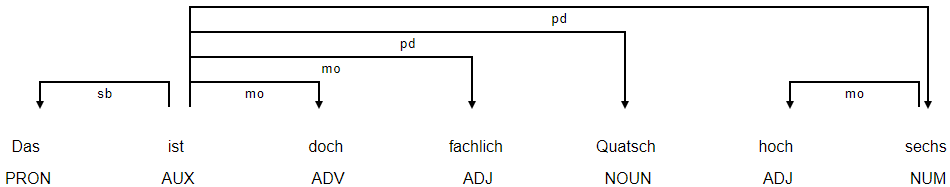
\includegraphics[width=1\textwidth]{chapters/04-Sentiment-Analyse/steffi.png}}
\caption{Visualisierung der Wortabhängigkeiten (Zitat von Steffi Lemke MdB, 208. Sitzung, 10.02.2021)}
\label{steffi}
\end{figure}

\subsection{Negations-Erkennung}
\label{neg-erkennung}
Negation, also Ablehnung, Verneinung oder Aufhebung, hat einen erheblichen Einfluss auf das Ergebnis und damit die Korrektheit der Sentimentanalyse, weshalb in dieser Arbeit ein besonderes Augenmerk auf ihre Erkennung gelegt wurde. 
In \textit{Negation Modeling for German Polarity Classification} \cite{g3_wieg} präsentieren Forscher der Universität des Saarlandes und des Leibniz-Institut für Deutsche Sprache hierfür einen regelbasierten Ansatz. 

Sie definieren unterschiedliche Negationstypen und ihre jeweilige Reichweite. 
So beeinflussen etwa negierende Adverbien oder Indefinitpronomen wie \textit{nie} den gesamten Satz, wohingegen das Partikel \textit{nicht} lediglich seinen Vorgänger negiert.  
Die Tabelle \ref{g3tab1} führt alle in dieser Arbeit implementierten Negationsregeln auf. 
Die Nutzung eines Abhängigkeitsbaumes, wie von \mintinline{latex}{spaCy} ermittelt, ist dabei unerlässlich. 
Denn wie schon im vorherigen Kapitel angesprochen, ist etwa mit dem Vorgänger eines Wortes nicht das in der Satzabfolge voranstehende Wort gemeint, sondern vielmehr der semantische Regent. 

\begin{table}[htbp]
\caption{Implementierte Negations-Regeln aus \cite{g3_wieg}}
\begin{center}
\begin{tabular}{| c | c | c |}
\hline
\textbf{Negationstyp} & \textbf{Reichweite} & \textbf{Beispielworte} \\ \hline
Partikel & Vorgänger (Regent) & nicht \\ \hline
Präpositionen & Nachfolger (Dependent) & ohne, gegen \\ \hline
Adverbien, & Satz & nie, kein, kaum \\
Indefinitpronomen &  &  \\ \hline
Nomen & Genitiv,& Abschaffung, \\
 & Präpositionalobjekt & Zerstörung \\ \hline
Verben & Objekt, Subjekt & enden, sinken, lindern \\
\hline
\end{tabular}
\label{g3tab1}
\end{center}
\end{table}

Angemerkt sei an dieser Stelle, dass es nicht möglich war, alle Regeln aus \cite{g3_wieg} zu implementieren, da der von den Forschern genutzte Dependency-Parser umfangreichere Ergebnisse liefert, als jener von \mintinline{latex}{spaCy}. 

Eine Liste mit Negationsworten und dem jeweiligen Negationstyp wurde \cite{g3_polcla} entnommen und ist ebenfalls über die Klasse \mintinline{latex}{Lexicon} zugreifbar. 
Die Klasse stellt ein \mintinline{latex}{Dictionary} bereit, in welchem die Schlüssel die Negationsworte und die Werte eine Liste der Reichweiten sind. 

Wenn in einem Text ein Negationswort auftritt, werden alle implementierten Regeln geprüft. 
Sollte es zu einem Treffer kommen, etwa wenn das Wort \textit{nicht} auftritt (siehe Abb. \ref{brandner}) und es einen Vorgänger gibt, werden alle Worte in Reichweite des Negationswortes negiert. 
Dies geschieht, indem für die jeweiligen Worte, welche wie in \ref{g3textv} beschrieben \mintinline{latex}{Token}-Objekte sind, ein eigenes Attribut mit der Bezeichnung \mintinline{latex}{negated} auf \mintinline{latex}{True} gesetzt wird. 
In der Polaritätsberechnung wird wortweise auf dieses Attribut geprüft und die Wort-Polarität bei einer Negierung mit -1 multipliziert. 

\begin{figure}[htb]
\centerline{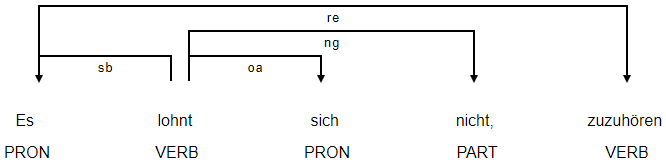
\includegraphics[width=1\textwidth]{chapters/04-Sentiment-Analyse/brandner.png}}
\caption{Beispielsatz mit Patikel-Negation (Zitat von Stephan Brandner MdB, 207. Sitzung, 29.01.2021)}
\label{brandner}
\end{figure}

\subsection{Verstärkungs-Erkennung}
\label{ver-erkennung}
Als \textit{Verstärker} werden sog. Gradpartikel (z.B. sehr, besonders, viel) verstanden, welche direkt vor Adjektiven oder Adverbien in einem Satz auftreten. 
Sie verstärken ihren Nachfolger, was wiederum in der Polaritätsberechnung berücksichtigt werden soll. 

Aus diesem Grund wird eine Liste mit verstärkenden Gradpartikeln, welche ebenfalls aus \cite{g3_polcla} bezogen werden, eingelesen und über die \mintinline{latex}{Lexicon} Klasse bereitgestellt. 

Ebenso wie in Kapitel \ref{neg-erkennung} bereits für die Negation beschrieben, wird ein eigenes Attribut zur Signalisierung einer Verstärkung definiert und im entsprechenden Fall auf True gesetzt. 
Bei der Polaritätsberechnung wird bei einer erkannten Verstärkung die Wort-Polarität mit 1,5 multipliziert \cite{g3_sentia}. 

In Abbildung \ref{hessel} wird ein Beispiel für das Auftreten eines verstärkenden Gradpartikels gegeben. 
Hier verstärkt das Wort \textit{sehr} das negative Wort \textit{spät}, womit die errechnete Polarität stärker negativ ausfällt als ohne die Verstärkungs-Erkennung. 

\begin{figure}[htb]
\centerline{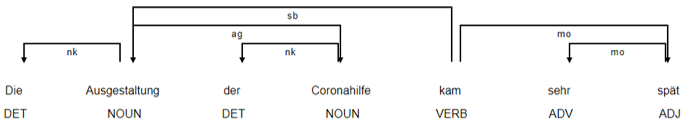
\includegraphics[width=1\textwidth]{chapters/04-Sentiment-Analyse/hessel.png}}
\caption{Beispielsatz mit Gradpartikel-Verstärkung (Zitat von Katja Hessel MdB, 206. Sitzung, 28.01.2021)}
\label{hessel}
\end{figure}

\subsection{Polaritätsberechnung}
\label{polberechnung}
Für die abschließende Berechnung der Polarität sind verschiedene Formeln denkbar. 
Sie sollten anhand von Textcharakteristika wie z.B. der Satz- oder Textlänge gewählt werden. 

Bei der Verwendung einer satzbasierten Polaritätsberechnung, bei welcher alle Polaritäten erst addiert und die Summe anschließend durch die Anzahl der Worte dividiert wird, kann ein unerwünschtes Phänomen auftreten: 
Längere Sätze erhaltenen ein stärker polarisiertes Ergebnis als vergleichbare kurze Sätze. 

Dies ist mit einer im Schnitt höheren Dichte an Worten mit Polaritäts-Wert in längeren Sätzen zu erklären. 
Um diesem Problem entgegen zu wirken, wurde in dieser Arbeit eine Min-Max-Skalierung (siehe Formeln 1 - 3) auf Dokumentebene implementiert \cite{g3_sentia}. 

Die Entscheidung, diese Normalisierung anhand der Länge des gesamten Textes durchzuführen, wurde aufgrund der Charakteristika der zu analysierenden Interaktionen getroffen. 
Denn diese bestehen zu einem überwiegenden Teil aus einem einzelnen Satz von jedoch sehr unterschiedlicher Länge. 

\begin{align}
p' &= \frac{ p + 1 }{ text.len + 1 } \text{ für p $>$ 0}\\
p' &= \frac{ p - 1 }{ text.len + 1 } \text{ für p $<$ 0}\\
p' &= p \text{ für p $=$ 0}
\end{align}

\section{Evaluierung}
\subsection{Sprache im Bundestag}
\label{sprachebundestag}
Während der Entwicklung dieser Arbeit und den regelmäßig angestellten Zwischentests wurde ersichtlich, dass sich die Sprache im Bundestag etwa von jener in sozialen Netzwerken oder Produktbewertungen unterschiedet. 
Ein Interaktionstext setzt sich sowohl aus einzelnen, langen und komplexe Sätze zusammen, als auch aus einzelnen Ausrufen wie \textit{\glqq eieiei!\grqq} zusammen. 

Aus diesem Grund wurde die in \ref{polberechnung} beschriebene Normalisierung verwendet, da herkömmliche Berechnungsformeln zunächst widersprüchliche Ergebnisse lieferten. 
Gleichzeitig verbesserte die manuelle Durchsicht der häufigsten 15.000 Worte und Anfertigung einer eigenen Bundestags-Wortliste das Ergebnis deutlich. 
Viele der regelmäßig in Bundestagssitzungen verwendeten Worte gehören zur \textit{Politik-Domäne} und treten deshalb nicht in den Quell-Wortlisten auf. 
Hier wird erwartet, dass eine noch umfangreichere Bundestags-Wortliste einen weiteren positiven Einfluss auf das Endergebnis hätte. 
Aus Zeit- sowie Kompetenzgründen wurde diese Liste jedoch nicht erweitert. 

\subsection{Ironie und Sarkasmus}
Ebenso wie die im vorherigen besprochene \textit{Politiksprache}, treten auch Ironie und Sarkasmus vermehrt in den Sitzungen des Bundestages auf. 
Einfach umrissen, handelt es sich dabei um ein Stilmittel, bei dem das Gegenteil vom Gesagten gemeint ist. 
Sarkasmus ist dabei eine verstärkte Form der Ironie und kann auch als ein Angriff verstanden werden. 

Selbst für den menschlichen Leser ist allein am geschriebenen Text nicht immer ersichtlich, ob eine Aussage ironisch gemeint ist. 
Vielmehr wird für die richtige Deutung die Stimmlage, Gestik und Mimik der sprechenden Person benötigt. 

Ironie und Sarkasmus könne also erst recht nicht mit dem in dieser Arbeit verwendeten Wortlisten-Ansatz erkannt werden, womit ein unbekannter Teil der Interaktionen im Ergebnis die falsche Polarität besitzt. 
Gleichwohl gibt es Ansätze aus dem Bereich des maschinellen Lernens, welche dieses Problem behandeln. 
Jedoch setzen diese einen entsprechend annotierten Korpus vorraus und stammen zudem aus dem Bereich der sozialen Netzwerke, in welchen etwa mit \textit{Hashtags} die Ironie bereits vom Autor markiert wurde. 

\subsection{Fazit}
Trotzt der soeben beschriebenen Fehlerquellen, wurde dennoch ein gelungenes Ergebnis erzielt: 
Es wurde ein solider und erweiterbarer Algorithmus zur Sentimentananlyse von Texten geschaffen, welcher auf den bekanntesten Bibliotheken und Techniken der Textverarbeitung beruht. 
Dieser kann als Basis für weitere Anstrengungen bei der Sentimentanalyse von politischen Texten dienen. 

Eine Deutung der bisherigen Ergebnisse durch Politikwissenschaftler oder anderweitig in diesem Bereich kompetente Personen wird dabei empfohlen, um die beschriebenen Schwachstellen entsprechend zu behandeln oder neue zu identifizieren. 

Der Programmcode ist zudem vollständig und abgesichert in die Projektpipeline eingebunden. 
Er erweitert seine Ergebnis-Datenbank automatisch um neue Sitzungen und benachrichtigt anschließend nachfolgende Gruppen. 

\section{Grundlagen}\label{sec:07_02_grundlagen}
\section{Anforderungsanalyse und Konzept}\label{sec:08_03_anforderungen_konzept}


\section{Zusammenfassung und Ausblick}\label{sec:07_05_zusammenfassung}

\chapter{Sentiment Analyse}
\section{Einleitung}
Der Begriff \textit{Sentiment} stammt vom lateinischen Wort \textit{sentimentum} ab und bedeutet Empfindung oder Stimmung. 
In der Sentimentanalyse geht es um die Bestimmung eben jener Stimmung einer Meinungsäußerung. 
Anwendung findet sie etwa bei Produktbewertungen oder Beiträgen in sozialen Netzwerken. 
Die Stimmung wird durch die sog. Polarität beschrieben und kann positiv, negativ oder neutral ausfallen. 
Im Text-Mining wird sie im Intervall $\interval{-1}{1} = \{x \in \mathbb{R} | -1 \leq x \leq 1\}$ angegeben, wobei -1 sehr negativ, 1 sehr positiv und 0 neutral bedeuten. 

Grundlegend ist die maschinelle Sentimentanalyse entweder Wortlisten- oder Modell-basiert. 
Der Wortlisten-Ansatz kann als eine Sammlung von Worten und ihrer Polaritäten verstanden werden, anhand welcher die Stimmung berechnet wird. 
Dieser Ansatz wird weiter im Kapitel \ref{wortliste} beschrieben, da er in dieser Arbeit verwendet wurde. 

Bei der Modell-basierten Sentimentanalyse wird ein annotierter Satz-Korpus für das Trainieren einer künstlichen Intelligenz vorausgesetzt. 
Etwa für Twitter-Beiträge stehen solche Korpusse oder auch bereits trainierte Modelle zur Verfügung. 
Jedoch ist bei der Verwendung zur Analyse der Sitzungsprotokolle des Bundestages nicht mit zufriedenstellenden Ergebnissen zu rechnen, da sich verwendete Worte und Text- bzw. Satzbau zwischen diesen Domänen deutlich unterscheiden. 
Eine weitere Erläuterung zur Sprache im Bundestag wird in Kapitel \ref{sprachebundestag} gegeben. 

Ebenfalls werden die Komponenten zur Teilnahme an der Verarbeitungspipeline des Gesamtprojektes im nachfolgenden Kapitel \ref{g3daten} beschrieben. 

\section{Datenaustausch}
\label{g3daten}
\subsection{Datenimport}
Für das Erhalten von Daten wurde eine Methode implementiert, welche durch Angabe einer Sitzungs-ID die entsprechende Sitzung vom REST-API von Gruppe 2 abfragen kann. 
Diese Methode gibt jede Sitzung weiter an die in Kapitel \ref{g3textv} beschriebene Textverarbeitung und das Ergebnis schließlich an den in Kapitel \ref{g3export} beschriebenen Export-Code. 

Die Methode wird für zwei Fälle verwendet: 
Beim Normalfall sendet die Gruppe 2 eine Benachrichtigung mit einer Liste aller neuen Sitzungs-IDs an das REST-API im Code dieser Arbeit. 
Das REST-API wurde mit der Bibliothek \mintinline{latex}{Flask} \cite{g3_flask} entwickelt und besteht aus einer POST-Schnittstelle, welche auf dem von der HTW bereitgestelltem Server unter \textit{/notify} erreichbar ist. 

Das API wurde unter Zuhilfenahme von \mintinline{latex}{Flask.Blueprints} \cite{g3_flaskbp} entwickelt und wird von einem \mintinline{latex}{Waitress}-Webserver \cite{g3_waitress} bereitgestellt. 
Für jede Anfrage wird geprüft, ob Content-Type und Payload dem erwarteten JSON-Daten entsprechen. 
Sollte dies nicht der Fall sein, wird eine entsprechende Rückmeldung an den Sender zurückgegeben. 
Für jede erhaltene Sitzungs-ID wird die eingangs beschriebene Methode aufgerufen. 

Der zweite Fall wurde vor allem im Rahmen der voranschreitenden Entwicklung bei den in der Projektpipeline voranstehenden Gruppen verwendet. 
Statt auf eine Benachrichtigung zum Anstoßen des Datenimports zu warten, werden stattdessen alle Sitzungs-IDs vom REST-API der Gruppe 2 abgefragt und jede Sitzung vollständig neu importiert. 
Dieses Vorgehen hat den Vorteil, dass eventuell durch Arbeit am Code verpasste Benachrichtigungen nachgeholt werden und gleichzeitig Änderungen an den Daten übernommen werden können. 

\subsection{Datenexport}
\label{g3export}
Statt Arbeit in ein umfangreiches REST-API für die nachfolgenden Gruppen zu stecken, wurde für diese Arbeit ein reiner MongoDB-Ansatz verwendet. 
Auf dem zur Verfügung stehenden HTW-Server wurde dafür eine MongoDB Instanz aufgesetzt, welche nur aus dem HTW-Netz erreichbar und zudem nur mit Authentifizierung zugreifbar ist. 
Jede Sitzung ist hier als eine eigene Collection persistiert. 
Sobald neue Sitzungen importiert und verarbeitet wurden, werden diese zunächst mit dem MongoDB-Treiber \mintinline{latex}{PyMongo} \cite{g3_mongodb} in die Datenbank geschrieben. 
Anschließend werden die nachfolgenden Gruppen mit einem POST and die jeweilige REST-Schnittstelle benachrichtigt, dass neue Daten vorliegen. 
Diese greifen dann mit den zuvor versendeten Zugangsdaten direkt auf die Datenbank zu. 

Mit diesem Vorgehen konnte die Komplexität beim Zugriff auf die Ergebnis-Daten gesenkt werden, da es für nahezu alle gängigen Programmiersprachen einen intuitiven MongoDB-Treiber gibt. 

\section{Wortliste}
\label{wortliste}
Wie bereits in der Einleitung beschrieben, handelt es sich bei Wortlisten in der Sentimentanalyse um eine Liste von Worten und ihrer jeweiligen Polarität. 
Bei der Analyse eines Textes wird wortweise ein Abgleich mit dieser Liste durchgeführt und die Wort-Polarität bei einer Übereinstimmung für die Berechnung des Sentiments verwendet. 
Unterschiedliche Berechnungsformeln sind dabei denkbar und werden in Kapitel \ref{polberechnung} weiter besprochen. 
Für diese Arbeit wurden Wortlisten verschiedener Institutionen kombiniert und anschließend mit Synonymen erweitert. 
Ebenfalls wurde eine eigene Bundestags-Wortliste erstellt. 

Die Interest Group on German Sentiment Analysis (IGGSA) stellt eine umfangreiche Liste an Publikationen und Ressourcen zu Sentimentanalysen in der deutschen Sprache zur Verfügung \cite{g3_iggsa}. 
Hier wurden alle Referenzen auf die in dieser Arbeit verwendeten Quell-Wortlisten gesammelt. 
Für die Zusammenführung dieser Wortlisten wurden zunächst zwei Herangehensweisen evaluiert: 
Zum einen war die Erstellung eines eigenständigen Codes denkbar, welcher einmalig die Daten aus allen Quellen einliest, zusammenfasst und eine Ergebnis-Datei ausgibt. 
Diese Datei wäre eine Ressource für den eigentlichen Analyse-Code. 
Zum anderen könnte die soeben beschriebene Funktionalität jedoch auch direkt im Analyse-Code integriert und bei jedem Programmstart ausgeführt werden. 
Die kombinierte Wortliste würde somit nicht auf die Festplatte geschrieben, sondern im Arbeitsspeicher verbleiben, solange der Analyse-Code läuft. 
Wenngleich der zuerst beschriebene Ansatz offensichtlich weniger Rechenzeitaufwändig ist, wurde für diese Arbeit der zweite Ansatz gewählt. 
Dies wird vor allem mit Rechtsunsicherheiten bei der Arbeit mit den verschiedenen Lizenzen der Quelldateien begründet. 
Gleichzeitig arbeitet der Analyse-Code damit jederzeit mit dem aktuellen Stand der Quell-Wortlisten. 
Das Aufbauen der Wortliste dauert wenige Minuten. 

Für diese Arbeit wurden die folgenden Quell-Wortlisten verwendet: 

\begin{itemize}
\item \textit{SentimentWortschatz} (SentiWS) aus \glqq SentiWS - a Publicly Available German-language Resource for Sentiment Analysis\grqq (Universität Leipzig) \cite{g3_sentiws}
\item \textit{Multi-Domain Sentiment Lexicon for German} (Hochschule Darmstadt) \cite{g3_opm}
\item \textit{German Polarity Lexicon} aus \glqq Evaluation and extension of a polarity lexicon for German\grqq (Universität Zürich) \cite{g3_polcla}
\item \textit{morphcomp} aus \glqq Evaluating the morphological compositionality of pola-rity\grqq (Leibniz-Institut für Deutsche Sprache, Universität des Saarlandes) \cite{g3_morphcomp}
\end{itemize}

Aus diesen Quellen ergibt sich eine Wortliste mit etwa 14.000 einzigartigen Worten. 
Die Worte werden dabei mit der in Kapitel \ref{g3textv} beschriebenen Textverarbeitungspipeline lemmatisiert, also auf die Grundform zurückgeführt. 
Bei Überschneidungen wird ein Mittelwert über alle Polaritäts-Werte eines Wortes gebildet. 

Mithilfe des \textit{Open German WordNet} (OdeNet) \cite{g3_odenet} werden zu jedem Wort Synonyme gesammelt und ebenfalls der Wortliste hinzugefügt. 
Der Zugriff auf OdeNet geschieht dabei mit der python Bibliothek \mintinline{latex}{WN} \cite{g3_wn}. 
Die Verwendung dieser Bibliothek ist trivial, weshalb an dieser Stelle keine weitere Erläuterung gegeben wird. 
Die Wortliste wird durch das Hinzufügen von Synonymen um weitere rund 2.000 Worte erweitert. 

Wie bereits in der Einleitung erwähnt, wurde zudem eine eigene Bundes-tags-Wortliste erstellt. 
Hierzu wurden die 15.000 am häufigsten in den Sitzungsprotokollen vorkommenden Worte erfasst und analysiert. 
Dabei wurden jedoch nur jene Worte betrachtet, welche nicht bereits in der kombinierten Wortliste vorkommen. 
Ausgewählt wurden nur eindeutig positive oder negative Worte wie \textit{angemessen}, \textit{Bullshit}, \textit{Fehlentscheidung}, \textit{Milchmädchenrechnung}, \textit{Realitätsverweigerung}, \textit{Totalausfall} oder \textit{Verunglimpfung}. 
Insgesamt umfasst die Bundestags-Wortliste 217 Worte. 

Im Code wird der Zugriff auf die Wortliste mit der zentralen Klasse \mintinline{latex}{Lexicon} realisiert. 
Bei der Instanziierung der Klasse werden, wie im Vorherigen beschrieben, alle Wortlisten gesammelt, zusammengeführt und erweitert. 
Anschließend stellt die Klasse ein \mintinline{latex}{Dictionary} bereit, in welchem die Schlüssel die Worte und die Werte die Wort-Polarität angeben. 

\section{Textverarbeitung}
\label{g3textv}
Für die Textverarbeitung nutzt der Code dieser Arbeit vollständig die Funktionalitäten und Strukturen von \mintinline{latex}{spaCy} \cite{g3_spacy}. 
Die \mintinline{latex}{spaCy} Bibliothek stellt eine Textverarbeitungspipeline bereit, welche mithilfe eines vortrainierten Modells funktioniert. 
Für die deutsche Sprache wurde ein solches Modell mit dem TIGER Korpus der Universität Stuttgart trainiert. 
Der Korpus umfasst ca. 50.000 Sätze aus Texten der Frankfurter Rundschau. 
Die \mintinline{latex}{spaCy}-Pipeline besteht aus den folgenden Komponenten: 

\begin{itemize}
\item Tokenisierung (Text- und Satzzerteilung)
\item POS-Tagging (Wortartenerkennung)
\item Dependency-Parsing (Wortabhängigkeitenerkennung)
\item Lemmatisierung (Wortgrundformermittlung)
\item Entity-Recognition (Eigennamenerkennung)
\end{itemize}

Das Ergebnis der Pipeline ist ein \mintinline{latex}{Doc}-Objekt, welches das Ergebnis des gesamten in die Pipeline gegebenen Textes umfasst. 
Einzelne Sätze innerhalb des \mintinline{latex}{Doc}-Objektes werden mit \mintinline{latex}{Span}-Objekten beschrieben und einzelne Worte mit \mintinline{latex}{Token}-Objekten. 
Die Objekttypen besitzen jeweils eigene Methoden und Erweiterungsmöglichkeiten in Form von sog. \textit{extension attributes}. 

Sehr einfach und gleichzeitig umfangreich kann die \mintinline{latex}{spaCy}-Pipeline an die eigenen Bedürfnisse angepasst werden. 
So wurde die Berechnung des Sentiments eines Textes direkt an die Komponenten der Standart-Pipeline angehängt. 
Logisch unterteilt sich diese in die Komponenten:

\begin{itemize}
\item Negations-Erkennung (siehe \ref{neg-erkennung})
\item Verstärkungs-Erkennung (siehe \ref{ver-erkennung})
\item Polaritätsberechnung (siehe \ref{polberechnung})
\end{itemize}

Basis für das nachfolgende Kapitel \ref{neg-erkennung} ist dabei das Ergebnis des Depen-dency-Parsers von \mintinline{latex}{spaCy}. 
Dieser bestimmt die Abhängigkeiten zwischen den einzelnen Elementen eines Satzes. 
Diese Funktion gehört dem Themenbereich der Dependenzgrammatik an, in welcher gerichtete Beziehungen zwischen den Worten eines Satzes beschreibt werden. 
Ein Wort kann einen Vorgänger (Regent) und mehrere Nachfolger (Dependenten) besitzen. 
Die Gesamtheit der Beziehungen eines Satzes wird auch Abhängigkeitsbaum genannt. 

Zur Verdeutlichung soll die Abbildung \ref{steffi} dienen, welche mithilfe von \mintinline{latex}{spaCy.displaCy} erstellt wurde. 
Zu sehen ist hier der Abhängigkeitsbaum des Satzes \textit{\glqq Das ist doch fachlich Quatsch hoch sechs!\grqq}. 
An den gerichteten Kanten befindet sich die Angabe des Satzgliedes, unterhalb der Worte die Angabe der Wortart. 

\begin{figure}[htb]
\centerline{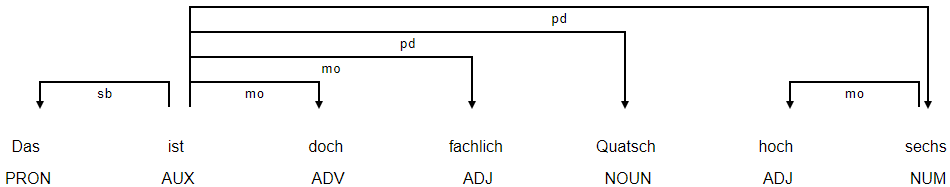
\includegraphics[width=1\textwidth]{chapters/04-Sentiment-Analyse/steffi.png}}
\caption{Visualisierung der Wortabhängigkeiten (Zitat von Steffi Lemke MdB, 208. Sitzung, 10.02.2021)}
\label{steffi}
\end{figure}

\subsection{Negations-Erkennung}
\label{neg-erkennung}
Negation, also Ablehnung, Verneinung oder Aufhebung, hat einen erheblichen Einfluss auf das Ergebnis und damit die Korrektheit der Sentimentanalyse, weshalb in dieser Arbeit ein besonderes Augenmerk auf ihre Erkennung gelegt wurde. 
In \textit{Negation Modeling for German Polarity Classification} \cite{g3_wieg} präsentieren Forscher der Universität des Saarlandes und des Leibniz-Institut für Deutsche Sprache hierfür einen regelbasierten Ansatz. 

Sie definieren unterschiedliche Negationstypen und ihre jeweilige Reichweite. 
So beeinflussen etwa negierende Adverbien oder Indefinitpronomen wie \textit{nie} den gesamten Satz, wohingegen das Partikel \textit{nicht} lediglich seinen Vorgänger negiert.  
Die Tabelle \ref{g3tab1} führt alle in dieser Arbeit implementierten Negationsregeln auf. 
Die Nutzung eines Abhängigkeitsbaumes, wie von \mintinline{latex}{spaCy} ermittelt, ist dabei unerlässlich. 
Denn wie schon im vorherigen Kapitel angesprochen, ist etwa mit dem Vorgänger eines Wortes nicht das in der Satzabfolge voranstehende Wort gemeint, sondern vielmehr der semantische Regent. 

\begin{table}[htbp]
\caption{Implementierte Negations-Regeln aus \cite{g3_wieg}}
\begin{center}
\begin{tabular}{| c | c | c |}
\hline
\textbf{Negationstyp} & \textbf{Reichweite} & \textbf{Beispielworte} \\ \hline
Partikel & Vorgänger (Regent) & nicht \\ \hline
Präpositionen & Nachfolger (Dependent) & ohne, gegen \\ \hline
Adverbien, & Satz & nie, kein, kaum \\
Indefinitpronomen &  &  \\ \hline
Nomen & Genitiv,& Abschaffung, \\
 & Präpositionalobjekt & Zerstörung \\ \hline
Verben & Objekt, Subjekt & enden, sinken, lindern \\
\hline
\end{tabular}
\label{g3tab1}
\end{center}
\end{table}

Angemerkt sei an dieser Stelle, dass es nicht möglich war, alle Regeln aus \cite{g3_wieg} zu implementieren, da der von den Forschern genutzte Dependency-Parser umfangreichere Ergebnisse liefert, als jener von \mintinline{latex}{spaCy}. 

Eine Liste mit Negationsworten und dem jeweiligen Negationstyp wurde \cite{g3_polcla} entnommen und ist ebenfalls über die Klasse \mintinline{latex}{Lexicon} zugreifbar. 
Die Klasse stellt ein \mintinline{latex}{Dictionary} bereit, in welchem die Schlüssel die Negationsworte und die Werte eine Liste der Reichweiten sind. 

Wenn in einem Text ein Negationswort auftritt, werden alle implementierten Regeln geprüft. 
Sollte es zu einem Treffer kommen, etwa wenn das Wort \textit{nicht} auftritt (siehe Abb. \ref{brandner}) und es einen Vorgänger gibt, werden alle Worte in Reichweite des Negationswortes negiert. 
Dies geschieht, indem für die jeweiligen Worte, welche wie in \ref{g3textv} beschrieben \mintinline{latex}{Token}-Objekte sind, ein eigenes Attribut mit der Bezeichnung \mintinline{latex}{negated} auf \mintinline{latex}{True} gesetzt wird. 
In der Polaritätsberechnung wird wortweise auf dieses Attribut geprüft und die Wort-Polarität bei einer Negierung mit -1 multipliziert. 

\begin{figure}[htb]
\centerline{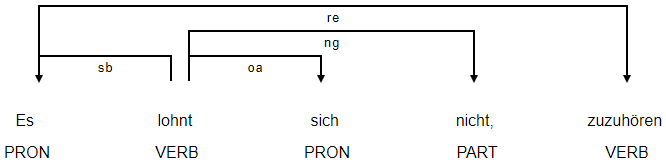
\includegraphics[width=1\textwidth]{chapters/04-Sentiment-Analyse/brandner.png}}
\caption{Beispielsatz mit Patikel-Negation (Zitat von Stephan Brandner MdB, 207. Sitzung, 29.01.2021)}
\label{brandner}
\end{figure}

\subsection{Verstärkungs-Erkennung}
\label{ver-erkennung}
Als \textit{Verstärker} werden sog. Gradpartikel (z.B. sehr, besonders, viel) verstanden, welche direkt vor Adjektiven oder Adverbien in einem Satz auftreten. 
Sie verstärken ihren Nachfolger, was wiederum in der Polaritätsberechnung berücksichtigt werden soll. 

Aus diesem Grund wird eine Liste mit verstärkenden Gradpartikeln, welche ebenfalls aus \cite{g3_polcla} bezogen werden, eingelesen und über die \mintinline{latex}{Lexicon} Klasse bereitgestellt. 

Ebenso wie in Kapitel \ref{neg-erkennung} bereits für die Negation beschrieben, wird ein eigenes Attribut zur Signalisierung einer Verstärkung definiert und im entsprechenden Fall auf True gesetzt. 
Bei der Polaritätsberechnung wird bei einer erkannten Verstärkung die Wort-Polarität mit 1,5 multipliziert \cite{g3_sentia}. 

In Abbildung \ref{hessel} wird ein Beispiel für das Auftreten eines verstärkenden Gradpartikels gegeben. 
Hier verstärkt das Wort \textit{sehr} das negative Wort \textit{spät}, womit die errechnete Polarität stärker negativ ausfällt als ohne die Verstärkungs-Erkennung. 

\begin{figure}[htb]
\centerline{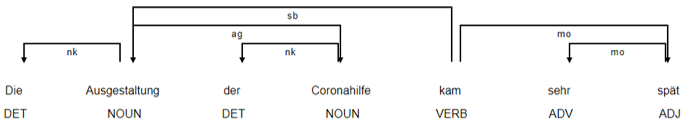
\includegraphics[width=1\textwidth]{chapters/04-Sentiment-Analyse/hessel.png}}
\caption{Beispielsatz mit Gradpartikel-Verstärkung (Zitat von Katja Hessel MdB, 206. Sitzung, 28.01.2021)}
\label{hessel}
\end{figure}

\subsection{Polaritätsberechnung}
\label{polberechnung}
Für die abschließende Berechnung der Polarität sind verschiedene Formeln denkbar. 
Sie sollten anhand von Textcharakteristika wie z.B. der Satz- oder Textlänge gewählt werden. 

Bei der Verwendung einer satzbasierten Polaritätsberechnung, bei welcher alle Polaritäten erst addiert und die Summe anschließend durch die Anzahl der Worte dividiert wird, kann ein unerwünschtes Phänomen auftreten: 
Längere Sätze erhaltenen ein stärker polarisiertes Ergebnis als vergleichbare kurze Sätze. 

Dies ist mit einer im Schnitt höheren Dichte an Worten mit Polaritäts-Wert in längeren Sätzen zu erklären. 
Um diesem Problem entgegen zu wirken, wurde in dieser Arbeit eine Min-Max-Skalierung (siehe Formeln 1 - 3) auf Dokumentebene implementiert \cite{g3_sentia}. 

Die Entscheidung, diese Normalisierung anhand der Länge des gesamten Textes durchzuführen, wurde aufgrund der Charakteristika der zu analysierenden Interaktionen getroffen. 
Denn diese bestehen zu einem überwiegenden Teil aus einem einzelnen Satz von jedoch sehr unterschiedlicher Länge. 

\begin{align}
p' &= \frac{ p + 1 }{ text.len + 1 } \text{ für p $>$ 0}\\
p' &= \frac{ p - 1 }{ text.len + 1 } \text{ für p $<$ 0}\\
p' &= p \text{ für p $=$ 0}
\end{align}

\section{Evaluierung}
\subsection{Sprache im Bundestag}
\label{sprachebundestag}
Während der Entwicklung dieser Arbeit und den regelmäßig angestellten Zwischentests wurde ersichtlich, dass sich die Sprache im Bundestag etwa von jener in sozialen Netzwerken oder Produktbewertungen unterschiedet. 
Ein Interaktionstext setzt sich sowohl aus einzelnen, langen und komplexe Sätze zusammen, als auch aus einzelnen Ausrufen wie \textit{\glqq eieiei!\grqq} zusammen. 

Aus diesem Grund wurde die in \ref{polberechnung} beschriebene Normalisierung verwendet, da herkömmliche Berechnungsformeln zunächst widersprüchliche Ergebnisse lieferten. 
Gleichzeitig verbesserte die manuelle Durchsicht der häufigsten 15.000 Worte und Anfertigung einer eigenen Bundestags-Wortliste das Ergebnis deutlich. 
Viele der regelmäßig in Bundestagssitzungen verwendeten Worte gehören zur \textit{Politik-Domäne} und treten deshalb nicht in den Quell-Wortlisten auf. 
Hier wird erwartet, dass eine noch umfangreichere Bundestags-Wortliste einen weiteren positiven Einfluss auf das Endergebnis hätte. 
Aus Zeit- sowie Kompetenzgründen wurde diese Liste jedoch nicht erweitert. 

\subsection{Ironie und Sarkasmus}
Ebenso wie die im vorherigen besprochene \textit{Politiksprache}, treten auch Ironie und Sarkasmus vermehrt in den Sitzungen des Bundestages auf. 
Einfach umrissen, handelt es sich dabei um ein Stilmittel, bei dem das Gegenteil vom Gesagten gemeint ist. 
Sarkasmus ist dabei eine verstärkte Form der Ironie und kann auch als ein Angriff verstanden werden. 

Selbst für den menschlichen Leser ist allein am geschriebenen Text nicht immer ersichtlich, ob eine Aussage ironisch gemeint ist. 
Vielmehr wird für die richtige Deutung die Stimmlage, Gestik und Mimik der sprechenden Person benötigt. 

Ironie und Sarkasmus könne also erst recht nicht mit dem in dieser Arbeit verwendeten Wortlisten-Ansatz erkannt werden, womit ein unbekannter Teil der Interaktionen im Ergebnis die falsche Polarität besitzt. 
Gleichwohl gibt es Ansätze aus dem Bereich des maschinellen Lernens, welche dieses Problem behandeln. 
Jedoch setzen diese einen entsprechend annotierten Korpus vorraus und stammen zudem aus dem Bereich der sozialen Netzwerke, in welchen etwa mit \textit{Hashtags} die Ironie bereits vom Autor markiert wurde. 

\subsection{Fazit}
Trotzt der soeben beschriebenen Fehlerquellen, wurde dennoch ein gelungenes Ergebnis erzielt: 
Es wurde ein solider und erweiterbarer Algorithmus zur Sentimentananlyse von Texten geschaffen, welcher auf den bekanntesten Bibliotheken und Techniken der Textverarbeitung beruht. 
Dieser kann als Basis für weitere Anstrengungen bei der Sentimentanalyse von politischen Texten dienen. 

Eine Deutung der bisherigen Ergebnisse durch Politikwissenschaftler oder anderweitig in diesem Bereich kompetente Personen wird dabei empfohlen, um die beschriebenen Schwachstellen entsprechend zu behandeln oder neue zu identifizieren. 

Der Programmcode ist zudem vollständig und abgesichert in die Projektpipeline eingebunden. 
Er erweitert seine Ergebnis-Datenbank automatisch um neue Sitzungen und benachrichtigt anschließend nachfolgende Gruppen. 

\section{Grundlagen}\label{sec:07_02_grundlagen}
\section{Anforderungsanalyse und Konzept}\label{sec:08_03_anforderungen_konzept}


\section{Zusammenfassung und Ausblick}\label{sec:07_05_zusammenfassung}

\chapter{Analyse der Interaktion zwischen Abgeordneten}
\section{Einleitung}
Der Begriff \textit{Sentiment} stammt vom lateinischen Wort \textit{sentimentum} ab und bedeutet Empfindung oder Stimmung. 
In der Sentimentanalyse geht es um die Bestimmung eben jener Stimmung einer Meinungsäußerung. 
Anwendung findet sie etwa bei Produktbewertungen oder Beiträgen in sozialen Netzwerken. 
Die Stimmung wird durch die sog. Polarität beschrieben und kann positiv, negativ oder neutral ausfallen. 
Im Text-Mining wird sie im Intervall $\interval{-1}{1} = \{x \in \mathbb{R} | -1 \leq x \leq 1\}$ angegeben, wobei -1 sehr negativ, 1 sehr positiv und 0 neutral bedeuten. 

Grundlegend ist die maschinelle Sentimentanalyse entweder Wortlisten- oder Modell-basiert. 
Der Wortlisten-Ansatz kann als eine Sammlung von Worten und ihrer Polaritäten verstanden werden, anhand welcher die Stimmung berechnet wird. 
Dieser Ansatz wird weiter im Kapitel \ref{wortliste} beschrieben, da er in dieser Arbeit verwendet wurde. 

Bei der Modell-basierten Sentimentanalyse wird ein annotierter Satz-Korpus für das Trainieren einer künstlichen Intelligenz vorausgesetzt. 
Etwa für Twitter-Beiträge stehen solche Korpusse oder auch bereits trainierte Modelle zur Verfügung. 
Jedoch ist bei der Verwendung zur Analyse der Sitzungsprotokolle des Bundestages nicht mit zufriedenstellenden Ergebnissen zu rechnen, da sich verwendete Worte und Text- bzw. Satzbau zwischen diesen Domänen deutlich unterscheiden. 
Eine weitere Erläuterung zur Sprache im Bundestag wird in Kapitel \ref{sprachebundestag} gegeben. 

Ebenfalls werden die Komponenten zur Teilnahme an der Verarbeitungspipeline des Gesamtprojektes im nachfolgenden Kapitel \ref{g3daten} beschrieben. 

\section{Datenaustausch}
\label{g3daten}
\subsection{Datenimport}
Für das Erhalten von Daten wurde eine Methode implementiert, welche durch Angabe einer Sitzungs-ID die entsprechende Sitzung vom REST-API von Gruppe 2 abfragen kann. 
Diese Methode gibt jede Sitzung weiter an die in Kapitel \ref{g3textv} beschriebene Textverarbeitung und das Ergebnis schließlich an den in Kapitel \ref{g3export} beschriebenen Export-Code. 

Die Methode wird für zwei Fälle verwendet: 
Beim Normalfall sendet die Gruppe 2 eine Benachrichtigung mit einer Liste aller neuen Sitzungs-IDs an das REST-API im Code dieser Arbeit. 
Das REST-API wurde mit der Bibliothek \mintinline{latex}{Flask} \cite{g3_flask} entwickelt und besteht aus einer POST-Schnittstelle, welche auf dem von der HTW bereitgestelltem Server unter \textit{/notify} erreichbar ist. 

Das API wurde unter Zuhilfenahme von \mintinline{latex}{Flask.Blueprints} \cite{g3_flaskbp} entwickelt und wird von einem \mintinline{latex}{Waitress}-Webserver \cite{g3_waitress} bereitgestellt. 
Für jede Anfrage wird geprüft, ob Content-Type und Payload dem erwarteten JSON-Daten entsprechen. 
Sollte dies nicht der Fall sein, wird eine entsprechende Rückmeldung an den Sender zurückgegeben. 
Für jede erhaltene Sitzungs-ID wird die eingangs beschriebene Methode aufgerufen. 

Der zweite Fall wurde vor allem im Rahmen der voranschreitenden Entwicklung bei den in der Projektpipeline voranstehenden Gruppen verwendet. 
Statt auf eine Benachrichtigung zum Anstoßen des Datenimports zu warten, werden stattdessen alle Sitzungs-IDs vom REST-API der Gruppe 2 abgefragt und jede Sitzung vollständig neu importiert. 
Dieses Vorgehen hat den Vorteil, dass eventuell durch Arbeit am Code verpasste Benachrichtigungen nachgeholt werden und gleichzeitig Änderungen an den Daten übernommen werden können. 

\subsection{Datenexport}
\label{g3export}
Statt Arbeit in ein umfangreiches REST-API für die nachfolgenden Gruppen zu stecken, wurde für diese Arbeit ein reiner MongoDB-Ansatz verwendet. 
Auf dem zur Verfügung stehenden HTW-Server wurde dafür eine MongoDB Instanz aufgesetzt, welche nur aus dem HTW-Netz erreichbar und zudem nur mit Authentifizierung zugreifbar ist. 
Jede Sitzung ist hier als eine eigene Collection persistiert. 
Sobald neue Sitzungen importiert und verarbeitet wurden, werden diese zunächst mit dem MongoDB-Treiber \mintinline{latex}{PyMongo} \cite{g3_mongodb} in die Datenbank geschrieben. 
Anschließend werden die nachfolgenden Gruppen mit einem POST and die jeweilige REST-Schnittstelle benachrichtigt, dass neue Daten vorliegen. 
Diese greifen dann mit den zuvor versendeten Zugangsdaten direkt auf die Datenbank zu. 

Mit diesem Vorgehen konnte die Komplexität beim Zugriff auf die Ergebnis-Daten gesenkt werden, da es für nahezu alle gängigen Programmiersprachen einen intuitiven MongoDB-Treiber gibt. 

\section{Wortliste}
\label{wortliste}
Wie bereits in der Einleitung beschrieben, handelt es sich bei Wortlisten in der Sentimentanalyse um eine Liste von Worten und ihrer jeweiligen Polarität. 
Bei der Analyse eines Textes wird wortweise ein Abgleich mit dieser Liste durchgeführt und die Wort-Polarität bei einer Übereinstimmung für die Berechnung des Sentiments verwendet. 
Unterschiedliche Berechnungsformeln sind dabei denkbar und werden in Kapitel \ref{polberechnung} weiter besprochen. 
Für diese Arbeit wurden Wortlisten verschiedener Institutionen kombiniert und anschließend mit Synonymen erweitert. 
Ebenfalls wurde eine eigene Bundestags-Wortliste erstellt. 

Die Interest Group on German Sentiment Analysis (IGGSA) stellt eine umfangreiche Liste an Publikationen und Ressourcen zu Sentimentanalysen in der deutschen Sprache zur Verfügung \cite{g3_iggsa}. 
Hier wurden alle Referenzen auf die in dieser Arbeit verwendeten Quell-Wortlisten gesammelt. 
Für die Zusammenführung dieser Wortlisten wurden zunächst zwei Herangehensweisen evaluiert: 
Zum einen war die Erstellung eines eigenständigen Codes denkbar, welcher einmalig die Daten aus allen Quellen einliest, zusammenfasst und eine Ergebnis-Datei ausgibt. 
Diese Datei wäre eine Ressource für den eigentlichen Analyse-Code. 
Zum anderen könnte die soeben beschriebene Funktionalität jedoch auch direkt im Analyse-Code integriert und bei jedem Programmstart ausgeführt werden. 
Die kombinierte Wortliste würde somit nicht auf die Festplatte geschrieben, sondern im Arbeitsspeicher verbleiben, solange der Analyse-Code läuft. 
Wenngleich der zuerst beschriebene Ansatz offensichtlich weniger Rechenzeitaufwändig ist, wurde für diese Arbeit der zweite Ansatz gewählt. 
Dies wird vor allem mit Rechtsunsicherheiten bei der Arbeit mit den verschiedenen Lizenzen der Quelldateien begründet. 
Gleichzeitig arbeitet der Analyse-Code damit jederzeit mit dem aktuellen Stand der Quell-Wortlisten. 
Das Aufbauen der Wortliste dauert wenige Minuten. 

Für diese Arbeit wurden die folgenden Quell-Wortlisten verwendet: 

\begin{itemize}
\item \textit{SentimentWortschatz} (SentiWS) aus \glqq SentiWS - a Publicly Available German-language Resource for Sentiment Analysis\grqq (Universität Leipzig) \cite{g3_sentiws}
\item \textit{Multi-Domain Sentiment Lexicon for German} (Hochschule Darmstadt) \cite{g3_opm}
\item \textit{German Polarity Lexicon} aus \glqq Evaluation and extension of a polarity lexicon for German\grqq (Universität Zürich) \cite{g3_polcla}
\item \textit{morphcomp} aus \glqq Evaluating the morphological compositionality of pola-rity\grqq (Leibniz-Institut für Deutsche Sprache, Universität des Saarlandes) \cite{g3_morphcomp}
\end{itemize}

Aus diesen Quellen ergibt sich eine Wortliste mit etwa 14.000 einzigartigen Worten. 
Die Worte werden dabei mit der in Kapitel \ref{g3textv} beschriebenen Textverarbeitungspipeline lemmatisiert, also auf die Grundform zurückgeführt. 
Bei Überschneidungen wird ein Mittelwert über alle Polaritäts-Werte eines Wortes gebildet. 

Mithilfe des \textit{Open German WordNet} (OdeNet) \cite{g3_odenet} werden zu jedem Wort Synonyme gesammelt und ebenfalls der Wortliste hinzugefügt. 
Der Zugriff auf OdeNet geschieht dabei mit der python Bibliothek \mintinline{latex}{WN} \cite{g3_wn}. 
Die Verwendung dieser Bibliothek ist trivial, weshalb an dieser Stelle keine weitere Erläuterung gegeben wird. 
Die Wortliste wird durch das Hinzufügen von Synonymen um weitere rund 2.000 Worte erweitert. 

Wie bereits in der Einleitung erwähnt, wurde zudem eine eigene Bundes-tags-Wortliste erstellt. 
Hierzu wurden die 15.000 am häufigsten in den Sitzungsprotokollen vorkommenden Worte erfasst und analysiert. 
Dabei wurden jedoch nur jene Worte betrachtet, welche nicht bereits in der kombinierten Wortliste vorkommen. 
Ausgewählt wurden nur eindeutig positive oder negative Worte wie \textit{angemessen}, \textit{Bullshit}, \textit{Fehlentscheidung}, \textit{Milchmädchenrechnung}, \textit{Realitätsverweigerung}, \textit{Totalausfall} oder \textit{Verunglimpfung}. 
Insgesamt umfasst die Bundestags-Wortliste 217 Worte. 

Im Code wird der Zugriff auf die Wortliste mit der zentralen Klasse \mintinline{latex}{Lexicon} realisiert. 
Bei der Instanziierung der Klasse werden, wie im Vorherigen beschrieben, alle Wortlisten gesammelt, zusammengeführt und erweitert. 
Anschließend stellt die Klasse ein \mintinline{latex}{Dictionary} bereit, in welchem die Schlüssel die Worte und die Werte die Wort-Polarität angeben. 

\section{Textverarbeitung}
\label{g3textv}
Für die Textverarbeitung nutzt der Code dieser Arbeit vollständig die Funktionalitäten und Strukturen von \mintinline{latex}{spaCy} \cite{g3_spacy}. 
Die \mintinline{latex}{spaCy} Bibliothek stellt eine Textverarbeitungspipeline bereit, welche mithilfe eines vortrainierten Modells funktioniert. 
Für die deutsche Sprache wurde ein solches Modell mit dem TIGER Korpus der Universität Stuttgart trainiert. 
Der Korpus umfasst ca. 50.000 Sätze aus Texten der Frankfurter Rundschau. 
Die \mintinline{latex}{spaCy}-Pipeline besteht aus den folgenden Komponenten: 

\begin{itemize}
\item Tokenisierung (Text- und Satzzerteilung)
\item POS-Tagging (Wortartenerkennung)
\item Dependency-Parsing (Wortabhängigkeitenerkennung)
\item Lemmatisierung (Wortgrundformermittlung)
\item Entity-Recognition (Eigennamenerkennung)
\end{itemize}

Das Ergebnis der Pipeline ist ein \mintinline{latex}{Doc}-Objekt, welches das Ergebnis des gesamten in die Pipeline gegebenen Textes umfasst. 
Einzelne Sätze innerhalb des \mintinline{latex}{Doc}-Objektes werden mit \mintinline{latex}{Span}-Objekten beschrieben und einzelne Worte mit \mintinline{latex}{Token}-Objekten. 
Die Objekttypen besitzen jeweils eigene Methoden und Erweiterungsmöglichkeiten in Form von sog. \textit{extension attributes}. 

Sehr einfach und gleichzeitig umfangreich kann die \mintinline{latex}{spaCy}-Pipeline an die eigenen Bedürfnisse angepasst werden. 
So wurde die Berechnung des Sentiments eines Textes direkt an die Komponenten der Standart-Pipeline angehängt. 
Logisch unterteilt sich diese in die Komponenten:

\begin{itemize}
\item Negations-Erkennung (siehe \ref{neg-erkennung})
\item Verstärkungs-Erkennung (siehe \ref{ver-erkennung})
\item Polaritätsberechnung (siehe \ref{polberechnung})
\end{itemize}

Basis für das nachfolgende Kapitel \ref{neg-erkennung} ist dabei das Ergebnis des Depen-dency-Parsers von \mintinline{latex}{spaCy}. 
Dieser bestimmt die Abhängigkeiten zwischen den einzelnen Elementen eines Satzes. 
Diese Funktion gehört dem Themenbereich der Dependenzgrammatik an, in welcher gerichtete Beziehungen zwischen den Worten eines Satzes beschreibt werden. 
Ein Wort kann einen Vorgänger (Regent) und mehrere Nachfolger (Dependenten) besitzen. 
Die Gesamtheit der Beziehungen eines Satzes wird auch Abhängigkeitsbaum genannt. 

Zur Verdeutlichung soll die Abbildung \ref{steffi} dienen, welche mithilfe von \mintinline{latex}{spaCy.displaCy} erstellt wurde. 
Zu sehen ist hier der Abhängigkeitsbaum des Satzes \textit{\glqq Das ist doch fachlich Quatsch hoch sechs!\grqq}. 
An den gerichteten Kanten befindet sich die Angabe des Satzgliedes, unterhalb der Worte die Angabe der Wortart. 

\begin{figure}[htb]
\centerline{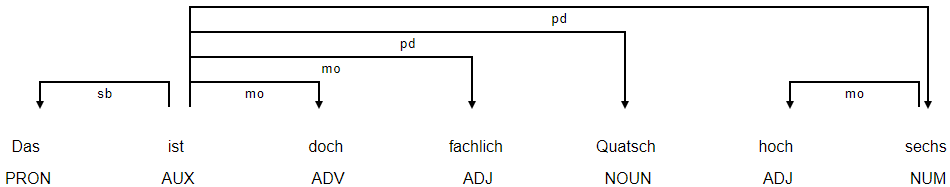
\includegraphics[width=1\textwidth]{chapters/04-Sentiment-Analyse/steffi.png}}
\caption{Visualisierung der Wortabhängigkeiten (Zitat von Steffi Lemke MdB, 208. Sitzung, 10.02.2021)}
\label{steffi}
\end{figure}

\subsection{Negations-Erkennung}
\label{neg-erkennung}
Negation, also Ablehnung, Verneinung oder Aufhebung, hat einen erheblichen Einfluss auf das Ergebnis und damit die Korrektheit der Sentimentanalyse, weshalb in dieser Arbeit ein besonderes Augenmerk auf ihre Erkennung gelegt wurde. 
In \textit{Negation Modeling for German Polarity Classification} \cite{g3_wieg} präsentieren Forscher der Universität des Saarlandes und des Leibniz-Institut für Deutsche Sprache hierfür einen regelbasierten Ansatz. 

Sie definieren unterschiedliche Negationstypen und ihre jeweilige Reichweite. 
So beeinflussen etwa negierende Adverbien oder Indefinitpronomen wie \textit{nie} den gesamten Satz, wohingegen das Partikel \textit{nicht} lediglich seinen Vorgänger negiert.  
Die Tabelle \ref{g3tab1} führt alle in dieser Arbeit implementierten Negationsregeln auf. 
Die Nutzung eines Abhängigkeitsbaumes, wie von \mintinline{latex}{spaCy} ermittelt, ist dabei unerlässlich. 
Denn wie schon im vorherigen Kapitel angesprochen, ist etwa mit dem Vorgänger eines Wortes nicht das in der Satzabfolge voranstehende Wort gemeint, sondern vielmehr der semantische Regent. 

\begin{table}[htbp]
\caption{Implementierte Negations-Regeln aus \cite{g3_wieg}}
\begin{center}
\begin{tabular}{| c | c | c |}
\hline
\textbf{Negationstyp} & \textbf{Reichweite} & \textbf{Beispielworte} \\ \hline
Partikel & Vorgänger (Regent) & nicht \\ \hline
Präpositionen & Nachfolger (Dependent) & ohne, gegen \\ \hline
Adverbien, & Satz & nie, kein, kaum \\
Indefinitpronomen &  &  \\ \hline
Nomen & Genitiv,& Abschaffung, \\
 & Präpositionalobjekt & Zerstörung \\ \hline
Verben & Objekt, Subjekt & enden, sinken, lindern \\
\hline
\end{tabular}
\label{g3tab1}
\end{center}
\end{table}

Angemerkt sei an dieser Stelle, dass es nicht möglich war, alle Regeln aus \cite{g3_wieg} zu implementieren, da der von den Forschern genutzte Dependency-Parser umfangreichere Ergebnisse liefert, als jener von \mintinline{latex}{spaCy}. 

Eine Liste mit Negationsworten und dem jeweiligen Negationstyp wurde \cite{g3_polcla} entnommen und ist ebenfalls über die Klasse \mintinline{latex}{Lexicon} zugreifbar. 
Die Klasse stellt ein \mintinline{latex}{Dictionary} bereit, in welchem die Schlüssel die Negationsworte und die Werte eine Liste der Reichweiten sind. 

Wenn in einem Text ein Negationswort auftritt, werden alle implementierten Regeln geprüft. 
Sollte es zu einem Treffer kommen, etwa wenn das Wort \textit{nicht} auftritt (siehe Abb. \ref{brandner}) und es einen Vorgänger gibt, werden alle Worte in Reichweite des Negationswortes negiert. 
Dies geschieht, indem für die jeweiligen Worte, welche wie in \ref{g3textv} beschrieben \mintinline{latex}{Token}-Objekte sind, ein eigenes Attribut mit der Bezeichnung \mintinline{latex}{negated} auf \mintinline{latex}{True} gesetzt wird. 
In der Polaritätsberechnung wird wortweise auf dieses Attribut geprüft und die Wort-Polarität bei einer Negierung mit -1 multipliziert. 

\begin{figure}[htb]
\centerline{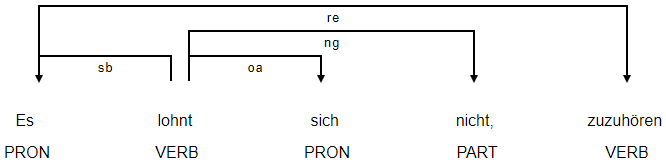
\includegraphics[width=1\textwidth]{chapters/04-Sentiment-Analyse/brandner.png}}
\caption{Beispielsatz mit Patikel-Negation (Zitat von Stephan Brandner MdB, 207. Sitzung, 29.01.2021)}
\label{brandner}
\end{figure}

\subsection{Verstärkungs-Erkennung}
\label{ver-erkennung}
Als \textit{Verstärker} werden sog. Gradpartikel (z.B. sehr, besonders, viel) verstanden, welche direkt vor Adjektiven oder Adverbien in einem Satz auftreten. 
Sie verstärken ihren Nachfolger, was wiederum in der Polaritätsberechnung berücksichtigt werden soll. 

Aus diesem Grund wird eine Liste mit verstärkenden Gradpartikeln, welche ebenfalls aus \cite{g3_polcla} bezogen werden, eingelesen und über die \mintinline{latex}{Lexicon} Klasse bereitgestellt. 

Ebenso wie in Kapitel \ref{neg-erkennung} bereits für die Negation beschrieben, wird ein eigenes Attribut zur Signalisierung einer Verstärkung definiert und im entsprechenden Fall auf True gesetzt. 
Bei der Polaritätsberechnung wird bei einer erkannten Verstärkung die Wort-Polarität mit 1,5 multipliziert \cite{g3_sentia}. 

In Abbildung \ref{hessel} wird ein Beispiel für das Auftreten eines verstärkenden Gradpartikels gegeben. 
Hier verstärkt das Wort \textit{sehr} das negative Wort \textit{spät}, womit die errechnete Polarität stärker negativ ausfällt als ohne die Verstärkungs-Erkennung. 

\begin{figure}[htb]
\centerline{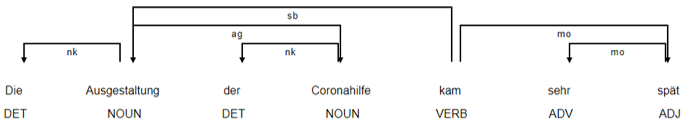
\includegraphics[width=1\textwidth]{chapters/04-Sentiment-Analyse/hessel.png}}
\caption{Beispielsatz mit Gradpartikel-Verstärkung (Zitat von Katja Hessel MdB, 206. Sitzung, 28.01.2021)}
\label{hessel}
\end{figure}

\subsection{Polaritätsberechnung}
\label{polberechnung}
Für die abschließende Berechnung der Polarität sind verschiedene Formeln denkbar. 
Sie sollten anhand von Textcharakteristika wie z.B. der Satz- oder Textlänge gewählt werden. 

Bei der Verwendung einer satzbasierten Polaritätsberechnung, bei welcher alle Polaritäten erst addiert und die Summe anschließend durch die Anzahl der Worte dividiert wird, kann ein unerwünschtes Phänomen auftreten: 
Längere Sätze erhaltenen ein stärker polarisiertes Ergebnis als vergleichbare kurze Sätze. 

Dies ist mit einer im Schnitt höheren Dichte an Worten mit Polaritäts-Wert in längeren Sätzen zu erklären. 
Um diesem Problem entgegen zu wirken, wurde in dieser Arbeit eine Min-Max-Skalierung (siehe Formeln 1 - 3) auf Dokumentebene implementiert \cite{g3_sentia}. 

Die Entscheidung, diese Normalisierung anhand der Länge des gesamten Textes durchzuführen, wurde aufgrund der Charakteristika der zu analysierenden Interaktionen getroffen. 
Denn diese bestehen zu einem überwiegenden Teil aus einem einzelnen Satz von jedoch sehr unterschiedlicher Länge. 

\begin{align}
p' &= \frac{ p + 1 }{ text.len + 1 } \text{ für p $>$ 0}\\
p' &= \frac{ p - 1 }{ text.len + 1 } \text{ für p $<$ 0}\\
p' &= p \text{ für p $=$ 0}
\end{align}

\section{Evaluierung}
\subsection{Sprache im Bundestag}
\label{sprachebundestag}
Während der Entwicklung dieser Arbeit und den regelmäßig angestellten Zwischentests wurde ersichtlich, dass sich die Sprache im Bundestag etwa von jener in sozialen Netzwerken oder Produktbewertungen unterschiedet. 
Ein Interaktionstext setzt sich sowohl aus einzelnen, langen und komplexe Sätze zusammen, als auch aus einzelnen Ausrufen wie \textit{\glqq eieiei!\grqq} zusammen. 

Aus diesem Grund wurde die in \ref{polberechnung} beschriebene Normalisierung verwendet, da herkömmliche Berechnungsformeln zunächst widersprüchliche Ergebnisse lieferten. 
Gleichzeitig verbesserte die manuelle Durchsicht der häufigsten 15.000 Worte und Anfertigung einer eigenen Bundestags-Wortliste das Ergebnis deutlich. 
Viele der regelmäßig in Bundestagssitzungen verwendeten Worte gehören zur \textit{Politik-Domäne} und treten deshalb nicht in den Quell-Wortlisten auf. 
Hier wird erwartet, dass eine noch umfangreichere Bundestags-Wortliste einen weiteren positiven Einfluss auf das Endergebnis hätte. 
Aus Zeit- sowie Kompetenzgründen wurde diese Liste jedoch nicht erweitert. 

\subsection{Ironie und Sarkasmus}
Ebenso wie die im vorherigen besprochene \textit{Politiksprache}, treten auch Ironie und Sarkasmus vermehrt in den Sitzungen des Bundestages auf. 
Einfach umrissen, handelt es sich dabei um ein Stilmittel, bei dem das Gegenteil vom Gesagten gemeint ist. 
Sarkasmus ist dabei eine verstärkte Form der Ironie und kann auch als ein Angriff verstanden werden. 

Selbst für den menschlichen Leser ist allein am geschriebenen Text nicht immer ersichtlich, ob eine Aussage ironisch gemeint ist. 
Vielmehr wird für die richtige Deutung die Stimmlage, Gestik und Mimik der sprechenden Person benötigt. 

Ironie und Sarkasmus könne also erst recht nicht mit dem in dieser Arbeit verwendeten Wortlisten-Ansatz erkannt werden, womit ein unbekannter Teil der Interaktionen im Ergebnis die falsche Polarität besitzt. 
Gleichwohl gibt es Ansätze aus dem Bereich des maschinellen Lernens, welche dieses Problem behandeln. 
Jedoch setzen diese einen entsprechend annotierten Korpus vorraus und stammen zudem aus dem Bereich der sozialen Netzwerke, in welchen etwa mit \textit{Hashtags} die Ironie bereits vom Autor markiert wurde. 

\subsection{Fazit}
Trotzt der soeben beschriebenen Fehlerquellen, wurde dennoch ein gelungenes Ergebnis erzielt: 
Es wurde ein solider und erweiterbarer Algorithmus zur Sentimentananlyse von Texten geschaffen, welcher auf den bekanntesten Bibliotheken und Techniken der Textverarbeitung beruht. 
Dieser kann als Basis für weitere Anstrengungen bei der Sentimentanalyse von politischen Texten dienen. 

Eine Deutung der bisherigen Ergebnisse durch Politikwissenschaftler oder anderweitig in diesem Bereich kompetente Personen wird dabei empfohlen, um die beschriebenen Schwachstellen entsprechend zu behandeln oder neue zu identifizieren. 

Der Programmcode ist zudem vollständig und abgesichert in die Projektpipeline eingebunden. 
Er erweitert seine Ergebnis-Datenbank automatisch um neue Sitzungen und benachrichtigt anschließend nachfolgende Gruppen. 

\section{Grundlagen}\label{sec:07_02_grundlagen}
\section{Anforderungsanalyse und Konzept}\label{sec:08_03_anforderungen_konzept}


\section{Zusammenfassung und Ausblick}\label{sec:07_05_zusammenfassung}

\chapter{Analyse der Interaktion zwischen Fraktionen}
\section{Einleitung}
Der Begriff \textit{Sentiment} stammt vom lateinischen Wort \textit{sentimentum} ab und bedeutet Empfindung oder Stimmung. 
In der Sentimentanalyse geht es um die Bestimmung eben jener Stimmung einer Meinungsäußerung. 
Anwendung findet sie etwa bei Produktbewertungen oder Beiträgen in sozialen Netzwerken. 
Die Stimmung wird durch die sog. Polarität beschrieben und kann positiv, negativ oder neutral ausfallen. 
Im Text-Mining wird sie im Intervall $\interval{-1}{1} = \{x \in \mathbb{R} | -1 \leq x \leq 1\}$ angegeben, wobei -1 sehr negativ, 1 sehr positiv und 0 neutral bedeuten. 

Grundlegend ist die maschinelle Sentimentanalyse entweder Wortlisten- oder Modell-basiert. 
Der Wortlisten-Ansatz kann als eine Sammlung von Worten und ihrer Polaritäten verstanden werden, anhand welcher die Stimmung berechnet wird. 
Dieser Ansatz wird weiter im Kapitel \ref{wortliste} beschrieben, da er in dieser Arbeit verwendet wurde. 

Bei der Modell-basierten Sentimentanalyse wird ein annotierter Satz-Korpus für das Trainieren einer künstlichen Intelligenz vorausgesetzt. 
Etwa für Twitter-Beiträge stehen solche Korpusse oder auch bereits trainierte Modelle zur Verfügung. 
Jedoch ist bei der Verwendung zur Analyse der Sitzungsprotokolle des Bundestages nicht mit zufriedenstellenden Ergebnissen zu rechnen, da sich verwendete Worte und Text- bzw. Satzbau zwischen diesen Domänen deutlich unterscheiden. 
Eine weitere Erläuterung zur Sprache im Bundestag wird in Kapitel \ref{sprachebundestag} gegeben. 

Ebenfalls werden die Komponenten zur Teilnahme an der Verarbeitungspipeline des Gesamtprojektes im nachfolgenden Kapitel \ref{g3daten} beschrieben. 

\section{Datenaustausch}
\label{g3daten}
\subsection{Datenimport}
Für das Erhalten von Daten wurde eine Methode implementiert, welche durch Angabe einer Sitzungs-ID die entsprechende Sitzung vom REST-API von Gruppe 2 abfragen kann. 
Diese Methode gibt jede Sitzung weiter an die in Kapitel \ref{g3textv} beschriebene Textverarbeitung und das Ergebnis schließlich an den in Kapitel \ref{g3export} beschriebenen Export-Code. 

Die Methode wird für zwei Fälle verwendet: 
Beim Normalfall sendet die Gruppe 2 eine Benachrichtigung mit einer Liste aller neuen Sitzungs-IDs an das REST-API im Code dieser Arbeit. 
Das REST-API wurde mit der Bibliothek \mintinline{latex}{Flask} \cite{g3_flask} entwickelt und besteht aus einer POST-Schnittstelle, welche auf dem von der HTW bereitgestelltem Server unter \textit{/notify} erreichbar ist. 

Das API wurde unter Zuhilfenahme von \mintinline{latex}{Flask.Blueprints} \cite{g3_flaskbp} entwickelt und wird von einem \mintinline{latex}{Waitress}-Webserver \cite{g3_waitress} bereitgestellt. 
Für jede Anfrage wird geprüft, ob Content-Type und Payload dem erwarteten JSON-Daten entsprechen. 
Sollte dies nicht der Fall sein, wird eine entsprechende Rückmeldung an den Sender zurückgegeben. 
Für jede erhaltene Sitzungs-ID wird die eingangs beschriebene Methode aufgerufen. 

Der zweite Fall wurde vor allem im Rahmen der voranschreitenden Entwicklung bei den in der Projektpipeline voranstehenden Gruppen verwendet. 
Statt auf eine Benachrichtigung zum Anstoßen des Datenimports zu warten, werden stattdessen alle Sitzungs-IDs vom REST-API der Gruppe 2 abgefragt und jede Sitzung vollständig neu importiert. 
Dieses Vorgehen hat den Vorteil, dass eventuell durch Arbeit am Code verpasste Benachrichtigungen nachgeholt werden und gleichzeitig Änderungen an den Daten übernommen werden können. 

\subsection{Datenexport}
\label{g3export}
Statt Arbeit in ein umfangreiches REST-API für die nachfolgenden Gruppen zu stecken, wurde für diese Arbeit ein reiner MongoDB-Ansatz verwendet. 
Auf dem zur Verfügung stehenden HTW-Server wurde dafür eine MongoDB Instanz aufgesetzt, welche nur aus dem HTW-Netz erreichbar und zudem nur mit Authentifizierung zugreifbar ist. 
Jede Sitzung ist hier als eine eigene Collection persistiert. 
Sobald neue Sitzungen importiert und verarbeitet wurden, werden diese zunächst mit dem MongoDB-Treiber \mintinline{latex}{PyMongo} \cite{g3_mongodb} in die Datenbank geschrieben. 
Anschließend werden die nachfolgenden Gruppen mit einem POST and die jeweilige REST-Schnittstelle benachrichtigt, dass neue Daten vorliegen. 
Diese greifen dann mit den zuvor versendeten Zugangsdaten direkt auf die Datenbank zu. 

Mit diesem Vorgehen konnte die Komplexität beim Zugriff auf die Ergebnis-Daten gesenkt werden, da es für nahezu alle gängigen Programmiersprachen einen intuitiven MongoDB-Treiber gibt. 

\section{Wortliste}
\label{wortliste}
Wie bereits in der Einleitung beschrieben, handelt es sich bei Wortlisten in der Sentimentanalyse um eine Liste von Worten und ihrer jeweiligen Polarität. 
Bei der Analyse eines Textes wird wortweise ein Abgleich mit dieser Liste durchgeführt und die Wort-Polarität bei einer Übereinstimmung für die Berechnung des Sentiments verwendet. 
Unterschiedliche Berechnungsformeln sind dabei denkbar und werden in Kapitel \ref{polberechnung} weiter besprochen. 
Für diese Arbeit wurden Wortlisten verschiedener Institutionen kombiniert und anschließend mit Synonymen erweitert. 
Ebenfalls wurde eine eigene Bundestags-Wortliste erstellt. 

Die Interest Group on German Sentiment Analysis (IGGSA) stellt eine umfangreiche Liste an Publikationen und Ressourcen zu Sentimentanalysen in der deutschen Sprache zur Verfügung \cite{g3_iggsa}. 
Hier wurden alle Referenzen auf die in dieser Arbeit verwendeten Quell-Wortlisten gesammelt. 
Für die Zusammenführung dieser Wortlisten wurden zunächst zwei Herangehensweisen evaluiert: 
Zum einen war die Erstellung eines eigenständigen Codes denkbar, welcher einmalig die Daten aus allen Quellen einliest, zusammenfasst und eine Ergebnis-Datei ausgibt. 
Diese Datei wäre eine Ressource für den eigentlichen Analyse-Code. 
Zum anderen könnte die soeben beschriebene Funktionalität jedoch auch direkt im Analyse-Code integriert und bei jedem Programmstart ausgeführt werden. 
Die kombinierte Wortliste würde somit nicht auf die Festplatte geschrieben, sondern im Arbeitsspeicher verbleiben, solange der Analyse-Code läuft. 
Wenngleich der zuerst beschriebene Ansatz offensichtlich weniger Rechenzeitaufwändig ist, wurde für diese Arbeit der zweite Ansatz gewählt. 
Dies wird vor allem mit Rechtsunsicherheiten bei der Arbeit mit den verschiedenen Lizenzen der Quelldateien begründet. 
Gleichzeitig arbeitet der Analyse-Code damit jederzeit mit dem aktuellen Stand der Quell-Wortlisten. 
Das Aufbauen der Wortliste dauert wenige Minuten. 

Für diese Arbeit wurden die folgenden Quell-Wortlisten verwendet: 

\begin{itemize}
\item \textit{SentimentWortschatz} (SentiWS) aus \glqq SentiWS - a Publicly Available German-language Resource for Sentiment Analysis\grqq (Universität Leipzig) \cite{g3_sentiws}
\item \textit{Multi-Domain Sentiment Lexicon for German} (Hochschule Darmstadt) \cite{g3_opm}
\item \textit{German Polarity Lexicon} aus \glqq Evaluation and extension of a polarity lexicon for German\grqq (Universität Zürich) \cite{g3_polcla}
\item \textit{morphcomp} aus \glqq Evaluating the morphological compositionality of pola-rity\grqq (Leibniz-Institut für Deutsche Sprache, Universität des Saarlandes) \cite{g3_morphcomp}
\end{itemize}

Aus diesen Quellen ergibt sich eine Wortliste mit etwa 14.000 einzigartigen Worten. 
Die Worte werden dabei mit der in Kapitel \ref{g3textv} beschriebenen Textverarbeitungspipeline lemmatisiert, also auf die Grundform zurückgeführt. 
Bei Überschneidungen wird ein Mittelwert über alle Polaritäts-Werte eines Wortes gebildet. 

Mithilfe des \textit{Open German WordNet} (OdeNet) \cite{g3_odenet} werden zu jedem Wort Synonyme gesammelt und ebenfalls der Wortliste hinzugefügt. 
Der Zugriff auf OdeNet geschieht dabei mit der python Bibliothek \mintinline{latex}{WN} \cite{g3_wn}. 
Die Verwendung dieser Bibliothek ist trivial, weshalb an dieser Stelle keine weitere Erläuterung gegeben wird. 
Die Wortliste wird durch das Hinzufügen von Synonymen um weitere rund 2.000 Worte erweitert. 

Wie bereits in der Einleitung erwähnt, wurde zudem eine eigene Bundes-tags-Wortliste erstellt. 
Hierzu wurden die 15.000 am häufigsten in den Sitzungsprotokollen vorkommenden Worte erfasst und analysiert. 
Dabei wurden jedoch nur jene Worte betrachtet, welche nicht bereits in der kombinierten Wortliste vorkommen. 
Ausgewählt wurden nur eindeutig positive oder negative Worte wie \textit{angemessen}, \textit{Bullshit}, \textit{Fehlentscheidung}, \textit{Milchmädchenrechnung}, \textit{Realitätsverweigerung}, \textit{Totalausfall} oder \textit{Verunglimpfung}. 
Insgesamt umfasst die Bundestags-Wortliste 217 Worte. 

Im Code wird der Zugriff auf die Wortliste mit der zentralen Klasse \mintinline{latex}{Lexicon} realisiert. 
Bei der Instanziierung der Klasse werden, wie im Vorherigen beschrieben, alle Wortlisten gesammelt, zusammengeführt und erweitert. 
Anschließend stellt die Klasse ein \mintinline{latex}{Dictionary} bereit, in welchem die Schlüssel die Worte und die Werte die Wort-Polarität angeben. 

\section{Textverarbeitung}
\label{g3textv}
Für die Textverarbeitung nutzt der Code dieser Arbeit vollständig die Funktionalitäten und Strukturen von \mintinline{latex}{spaCy} \cite{g3_spacy}. 
Die \mintinline{latex}{spaCy} Bibliothek stellt eine Textverarbeitungspipeline bereit, welche mithilfe eines vortrainierten Modells funktioniert. 
Für die deutsche Sprache wurde ein solches Modell mit dem TIGER Korpus der Universität Stuttgart trainiert. 
Der Korpus umfasst ca. 50.000 Sätze aus Texten der Frankfurter Rundschau. 
Die \mintinline{latex}{spaCy}-Pipeline besteht aus den folgenden Komponenten: 

\begin{itemize}
\item Tokenisierung (Text- und Satzzerteilung)
\item POS-Tagging (Wortartenerkennung)
\item Dependency-Parsing (Wortabhängigkeitenerkennung)
\item Lemmatisierung (Wortgrundformermittlung)
\item Entity-Recognition (Eigennamenerkennung)
\end{itemize}

Das Ergebnis der Pipeline ist ein \mintinline{latex}{Doc}-Objekt, welches das Ergebnis des gesamten in die Pipeline gegebenen Textes umfasst. 
Einzelne Sätze innerhalb des \mintinline{latex}{Doc}-Objektes werden mit \mintinline{latex}{Span}-Objekten beschrieben und einzelne Worte mit \mintinline{latex}{Token}-Objekten. 
Die Objekttypen besitzen jeweils eigene Methoden und Erweiterungsmöglichkeiten in Form von sog. \textit{extension attributes}. 

Sehr einfach und gleichzeitig umfangreich kann die \mintinline{latex}{spaCy}-Pipeline an die eigenen Bedürfnisse angepasst werden. 
So wurde die Berechnung des Sentiments eines Textes direkt an die Komponenten der Standart-Pipeline angehängt. 
Logisch unterteilt sich diese in die Komponenten:

\begin{itemize}
\item Negations-Erkennung (siehe \ref{neg-erkennung})
\item Verstärkungs-Erkennung (siehe \ref{ver-erkennung})
\item Polaritätsberechnung (siehe \ref{polberechnung})
\end{itemize}

Basis für das nachfolgende Kapitel \ref{neg-erkennung} ist dabei das Ergebnis des Depen-dency-Parsers von \mintinline{latex}{spaCy}. 
Dieser bestimmt die Abhängigkeiten zwischen den einzelnen Elementen eines Satzes. 
Diese Funktion gehört dem Themenbereich der Dependenzgrammatik an, in welcher gerichtete Beziehungen zwischen den Worten eines Satzes beschreibt werden. 
Ein Wort kann einen Vorgänger (Regent) und mehrere Nachfolger (Dependenten) besitzen. 
Die Gesamtheit der Beziehungen eines Satzes wird auch Abhängigkeitsbaum genannt. 

Zur Verdeutlichung soll die Abbildung \ref{steffi} dienen, welche mithilfe von \mintinline{latex}{spaCy.displaCy} erstellt wurde. 
Zu sehen ist hier der Abhängigkeitsbaum des Satzes \textit{\glqq Das ist doch fachlich Quatsch hoch sechs!\grqq}. 
An den gerichteten Kanten befindet sich die Angabe des Satzgliedes, unterhalb der Worte die Angabe der Wortart. 

\begin{figure}[htb]
\centerline{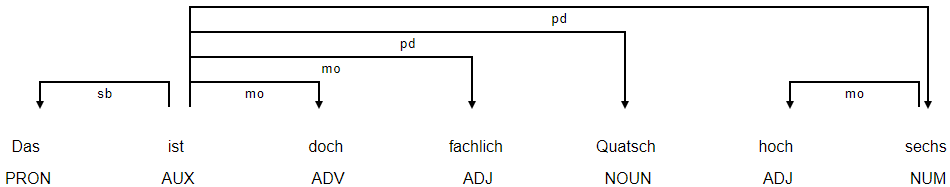
\includegraphics[width=1\textwidth]{chapters/04-Sentiment-Analyse/steffi.png}}
\caption{Visualisierung der Wortabhängigkeiten (Zitat von Steffi Lemke MdB, 208. Sitzung, 10.02.2021)}
\label{steffi}
\end{figure}

\subsection{Negations-Erkennung}
\label{neg-erkennung}
Negation, also Ablehnung, Verneinung oder Aufhebung, hat einen erheblichen Einfluss auf das Ergebnis und damit die Korrektheit der Sentimentanalyse, weshalb in dieser Arbeit ein besonderes Augenmerk auf ihre Erkennung gelegt wurde. 
In \textit{Negation Modeling for German Polarity Classification} \cite{g3_wieg} präsentieren Forscher der Universität des Saarlandes und des Leibniz-Institut für Deutsche Sprache hierfür einen regelbasierten Ansatz. 

Sie definieren unterschiedliche Negationstypen und ihre jeweilige Reichweite. 
So beeinflussen etwa negierende Adverbien oder Indefinitpronomen wie \textit{nie} den gesamten Satz, wohingegen das Partikel \textit{nicht} lediglich seinen Vorgänger negiert.  
Die Tabelle \ref{g3tab1} führt alle in dieser Arbeit implementierten Negationsregeln auf. 
Die Nutzung eines Abhängigkeitsbaumes, wie von \mintinline{latex}{spaCy} ermittelt, ist dabei unerlässlich. 
Denn wie schon im vorherigen Kapitel angesprochen, ist etwa mit dem Vorgänger eines Wortes nicht das in der Satzabfolge voranstehende Wort gemeint, sondern vielmehr der semantische Regent. 

\begin{table}[htbp]
\caption{Implementierte Negations-Regeln aus \cite{g3_wieg}}
\begin{center}
\begin{tabular}{| c | c | c |}
\hline
\textbf{Negationstyp} & \textbf{Reichweite} & \textbf{Beispielworte} \\ \hline
Partikel & Vorgänger (Regent) & nicht \\ \hline
Präpositionen & Nachfolger (Dependent) & ohne, gegen \\ \hline
Adverbien, & Satz & nie, kein, kaum \\
Indefinitpronomen &  &  \\ \hline
Nomen & Genitiv,& Abschaffung, \\
 & Präpositionalobjekt & Zerstörung \\ \hline
Verben & Objekt, Subjekt & enden, sinken, lindern \\
\hline
\end{tabular}
\label{g3tab1}
\end{center}
\end{table}

Angemerkt sei an dieser Stelle, dass es nicht möglich war, alle Regeln aus \cite{g3_wieg} zu implementieren, da der von den Forschern genutzte Dependency-Parser umfangreichere Ergebnisse liefert, als jener von \mintinline{latex}{spaCy}. 

Eine Liste mit Negationsworten und dem jeweiligen Negationstyp wurde \cite{g3_polcla} entnommen und ist ebenfalls über die Klasse \mintinline{latex}{Lexicon} zugreifbar. 
Die Klasse stellt ein \mintinline{latex}{Dictionary} bereit, in welchem die Schlüssel die Negationsworte und die Werte eine Liste der Reichweiten sind. 

Wenn in einem Text ein Negationswort auftritt, werden alle implementierten Regeln geprüft. 
Sollte es zu einem Treffer kommen, etwa wenn das Wort \textit{nicht} auftritt (siehe Abb. \ref{brandner}) und es einen Vorgänger gibt, werden alle Worte in Reichweite des Negationswortes negiert. 
Dies geschieht, indem für die jeweiligen Worte, welche wie in \ref{g3textv} beschrieben \mintinline{latex}{Token}-Objekte sind, ein eigenes Attribut mit der Bezeichnung \mintinline{latex}{negated} auf \mintinline{latex}{True} gesetzt wird. 
In der Polaritätsberechnung wird wortweise auf dieses Attribut geprüft und die Wort-Polarität bei einer Negierung mit -1 multipliziert. 

\begin{figure}[htb]
\centerline{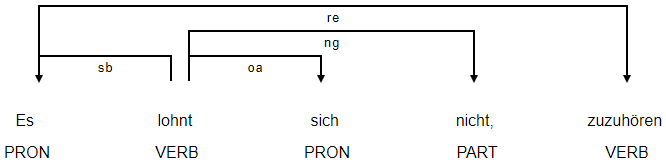
\includegraphics[width=1\textwidth]{chapters/04-Sentiment-Analyse/brandner.png}}
\caption{Beispielsatz mit Patikel-Negation (Zitat von Stephan Brandner MdB, 207. Sitzung, 29.01.2021)}
\label{brandner}
\end{figure}

\subsection{Verstärkungs-Erkennung}
\label{ver-erkennung}
Als \textit{Verstärker} werden sog. Gradpartikel (z.B. sehr, besonders, viel) verstanden, welche direkt vor Adjektiven oder Adverbien in einem Satz auftreten. 
Sie verstärken ihren Nachfolger, was wiederum in der Polaritätsberechnung berücksichtigt werden soll. 

Aus diesem Grund wird eine Liste mit verstärkenden Gradpartikeln, welche ebenfalls aus \cite{g3_polcla} bezogen werden, eingelesen und über die \mintinline{latex}{Lexicon} Klasse bereitgestellt. 

Ebenso wie in Kapitel \ref{neg-erkennung} bereits für die Negation beschrieben, wird ein eigenes Attribut zur Signalisierung einer Verstärkung definiert und im entsprechenden Fall auf True gesetzt. 
Bei der Polaritätsberechnung wird bei einer erkannten Verstärkung die Wort-Polarität mit 1,5 multipliziert \cite{g3_sentia}. 

In Abbildung \ref{hessel} wird ein Beispiel für das Auftreten eines verstärkenden Gradpartikels gegeben. 
Hier verstärkt das Wort \textit{sehr} das negative Wort \textit{spät}, womit die errechnete Polarität stärker negativ ausfällt als ohne die Verstärkungs-Erkennung. 

\begin{figure}[htb]
\centerline{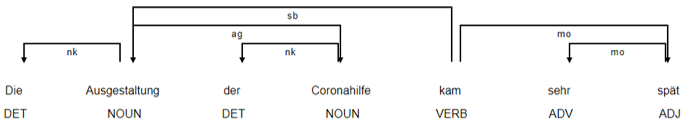
\includegraphics[width=1\textwidth]{chapters/04-Sentiment-Analyse/hessel.png}}
\caption{Beispielsatz mit Gradpartikel-Verstärkung (Zitat von Katja Hessel MdB, 206. Sitzung, 28.01.2021)}
\label{hessel}
\end{figure}

\subsection{Polaritätsberechnung}
\label{polberechnung}
Für die abschließende Berechnung der Polarität sind verschiedene Formeln denkbar. 
Sie sollten anhand von Textcharakteristika wie z.B. der Satz- oder Textlänge gewählt werden. 

Bei der Verwendung einer satzbasierten Polaritätsberechnung, bei welcher alle Polaritäten erst addiert und die Summe anschließend durch die Anzahl der Worte dividiert wird, kann ein unerwünschtes Phänomen auftreten: 
Längere Sätze erhaltenen ein stärker polarisiertes Ergebnis als vergleichbare kurze Sätze. 

Dies ist mit einer im Schnitt höheren Dichte an Worten mit Polaritäts-Wert in längeren Sätzen zu erklären. 
Um diesem Problem entgegen zu wirken, wurde in dieser Arbeit eine Min-Max-Skalierung (siehe Formeln 1 - 3) auf Dokumentebene implementiert \cite{g3_sentia}. 

Die Entscheidung, diese Normalisierung anhand der Länge des gesamten Textes durchzuführen, wurde aufgrund der Charakteristika der zu analysierenden Interaktionen getroffen. 
Denn diese bestehen zu einem überwiegenden Teil aus einem einzelnen Satz von jedoch sehr unterschiedlicher Länge. 

\begin{align}
p' &= \frac{ p + 1 }{ text.len + 1 } \text{ für p $>$ 0}\\
p' &= \frac{ p - 1 }{ text.len + 1 } \text{ für p $<$ 0}\\
p' &= p \text{ für p $=$ 0}
\end{align}

\section{Evaluierung}
\subsection{Sprache im Bundestag}
\label{sprachebundestag}
Während der Entwicklung dieser Arbeit und den regelmäßig angestellten Zwischentests wurde ersichtlich, dass sich die Sprache im Bundestag etwa von jener in sozialen Netzwerken oder Produktbewertungen unterschiedet. 
Ein Interaktionstext setzt sich sowohl aus einzelnen, langen und komplexe Sätze zusammen, als auch aus einzelnen Ausrufen wie \textit{\glqq eieiei!\grqq} zusammen. 

Aus diesem Grund wurde die in \ref{polberechnung} beschriebene Normalisierung verwendet, da herkömmliche Berechnungsformeln zunächst widersprüchliche Ergebnisse lieferten. 
Gleichzeitig verbesserte die manuelle Durchsicht der häufigsten 15.000 Worte und Anfertigung einer eigenen Bundestags-Wortliste das Ergebnis deutlich. 
Viele der regelmäßig in Bundestagssitzungen verwendeten Worte gehören zur \textit{Politik-Domäne} und treten deshalb nicht in den Quell-Wortlisten auf. 
Hier wird erwartet, dass eine noch umfangreichere Bundestags-Wortliste einen weiteren positiven Einfluss auf das Endergebnis hätte. 
Aus Zeit- sowie Kompetenzgründen wurde diese Liste jedoch nicht erweitert. 

\subsection{Ironie und Sarkasmus}
Ebenso wie die im vorherigen besprochene \textit{Politiksprache}, treten auch Ironie und Sarkasmus vermehrt in den Sitzungen des Bundestages auf. 
Einfach umrissen, handelt es sich dabei um ein Stilmittel, bei dem das Gegenteil vom Gesagten gemeint ist. 
Sarkasmus ist dabei eine verstärkte Form der Ironie und kann auch als ein Angriff verstanden werden. 

Selbst für den menschlichen Leser ist allein am geschriebenen Text nicht immer ersichtlich, ob eine Aussage ironisch gemeint ist. 
Vielmehr wird für die richtige Deutung die Stimmlage, Gestik und Mimik der sprechenden Person benötigt. 

Ironie und Sarkasmus könne also erst recht nicht mit dem in dieser Arbeit verwendeten Wortlisten-Ansatz erkannt werden, womit ein unbekannter Teil der Interaktionen im Ergebnis die falsche Polarität besitzt. 
Gleichwohl gibt es Ansätze aus dem Bereich des maschinellen Lernens, welche dieses Problem behandeln. 
Jedoch setzen diese einen entsprechend annotierten Korpus vorraus und stammen zudem aus dem Bereich der sozialen Netzwerke, in welchen etwa mit \textit{Hashtags} die Ironie bereits vom Autor markiert wurde. 

\subsection{Fazit}
Trotzt der soeben beschriebenen Fehlerquellen, wurde dennoch ein gelungenes Ergebnis erzielt: 
Es wurde ein solider und erweiterbarer Algorithmus zur Sentimentananlyse von Texten geschaffen, welcher auf den bekanntesten Bibliotheken und Techniken der Textverarbeitung beruht. 
Dieser kann als Basis für weitere Anstrengungen bei der Sentimentanalyse von politischen Texten dienen. 

Eine Deutung der bisherigen Ergebnisse durch Politikwissenschaftler oder anderweitig in diesem Bereich kompetente Personen wird dabei empfohlen, um die beschriebenen Schwachstellen entsprechend zu behandeln oder neue zu identifizieren. 

Der Programmcode ist zudem vollständig und abgesichert in die Projektpipeline eingebunden. 
Er erweitert seine Ergebnis-Datenbank automatisch um neue Sitzungen und benachrichtigt anschließend nachfolgende Gruppen. 

\section{Grundlagen}\label{sec:07_02_grundlagen}
\section{Anforderungsanalyse und Konzept}\label{sec:08_03_anforderungen_konzept}


\section{Zusammenfassung und Ausblick}\label{sec:07_05_zusammenfassung}

\chapter{Graphauswertung}
\normalsize \textsc{Ermittlung der Stimmungsmacher im Bundestag} \\
\normalsize \textsc{Markus Christopher Glutting, Marie Bittiehn, Miriam Lischke}
\section{Einleitung}
Der Begriff \textit{Sentiment} stammt vom lateinischen Wort \textit{sentimentum} ab und bedeutet Empfindung oder Stimmung. 
In der Sentimentanalyse geht es um die Bestimmung eben jener Stimmung einer Meinungsäußerung. 
Anwendung findet sie etwa bei Produktbewertungen oder Beiträgen in sozialen Netzwerken. 
Die Stimmung wird durch die sog. Polarität beschrieben und kann positiv, negativ oder neutral ausfallen. 
Im Text-Mining wird sie im Intervall $\interval{-1}{1} = \{x \in \mathbb{R} | -1 \leq x \leq 1\}$ angegeben, wobei -1 sehr negativ, 1 sehr positiv und 0 neutral bedeuten. 

Grundlegend ist die maschinelle Sentimentanalyse entweder Wortlisten- oder Modell-basiert. 
Der Wortlisten-Ansatz kann als eine Sammlung von Worten und ihrer Polaritäten verstanden werden, anhand welcher die Stimmung berechnet wird. 
Dieser Ansatz wird weiter im Kapitel \ref{wortliste} beschrieben, da er in dieser Arbeit verwendet wurde. 

Bei der Modell-basierten Sentimentanalyse wird ein annotierter Satz-Korpus für das Trainieren einer künstlichen Intelligenz vorausgesetzt. 
Etwa für Twitter-Beiträge stehen solche Korpusse oder auch bereits trainierte Modelle zur Verfügung. 
Jedoch ist bei der Verwendung zur Analyse der Sitzungsprotokolle des Bundestages nicht mit zufriedenstellenden Ergebnissen zu rechnen, da sich verwendete Worte und Text- bzw. Satzbau zwischen diesen Domänen deutlich unterscheiden. 
Eine weitere Erläuterung zur Sprache im Bundestag wird in Kapitel \ref{sprachebundestag} gegeben. 

Ebenfalls werden die Komponenten zur Teilnahme an der Verarbeitungspipeline des Gesamtprojektes im nachfolgenden Kapitel \ref{g3daten} beschrieben. 

\section{Datenaustausch}
\label{g3daten}
\subsection{Datenimport}
Für das Erhalten von Daten wurde eine Methode implementiert, welche durch Angabe einer Sitzungs-ID die entsprechende Sitzung vom REST-API von Gruppe 2 abfragen kann. 
Diese Methode gibt jede Sitzung weiter an die in Kapitel \ref{g3textv} beschriebene Textverarbeitung und das Ergebnis schließlich an den in Kapitel \ref{g3export} beschriebenen Export-Code. 

Die Methode wird für zwei Fälle verwendet: 
Beim Normalfall sendet die Gruppe 2 eine Benachrichtigung mit einer Liste aller neuen Sitzungs-IDs an das REST-API im Code dieser Arbeit. 
Das REST-API wurde mit der Bibliothek \mintinline{latex}{Flask} \cite{g3_flask} entwickelt und besteht aus einer POST-Schnittstelle, welche auf dem von der HTW bereitgestelltem Server unter \textit{/notify} erreichbar ist. 

Das API wurde unter Zuhilfenahme von \mintinline{latex}{Flask.Blueprints} \cite{g3_flaskbp} entwickelt und wird von einem \mintinline{latex}{Waitress}-Webserver \cite{g3_waitress} bereitgestellt. 
Für jede Anfrage wird geprüft, ob Content-Type und Payload dem erwarteten JSON-Daten entsprechen. 
Sollte dies nicht der Fall sein, wird eine entsprechende Rückmeldung an den Sender zurückgegeben. 
Für jede erhaltene Sitzungs-ID wird die eingangs beschriebene Methode aufgerufen. 

Der zweite Fall wurde vor allem im Rahmen der voranschreitenden Entwicklung bei den in der Projektpipeline voranstehenden Gruppen verwendet. 
Statt auf eine Benachrichtigung zum Anstoßen des Datenimports zu warten, werden stattdessen alle Sitzungs-IDs vom REST-API der Gruppe 2 abgefragt und jede Sitzung vollständig neu importiert. 
Dieses Vorgehen hat den Vorteil, dass eventuell durch Arbeit am Code verpasste Benachrichtigungen nachgeholt werden und gleichzeitig Änderungen an den Daten übernommen werden können. 

\subsection{Datenexport}
\label{g3export}
Statt Arbeit in ein umfangreiches REST-API für die nachfolgenden Gruppen zu stecken, wurde für diese Arbeit ein reiner MongoDB-Ansatz verwendet. 
Auf dem zur Verfügung stehenden HTW-Server wurde dafür eine MongoDB Instanz aufgesetzt, welche nur aus dem HTW-Netz erreichbar und zudem nur mit Authentifizierung zugreifbar ist. 
Jede Sitzung ist hier als eine eigene Collection persistiert. 
Sobald neue Sitzungen importiert und verarbeitet wurden, werden diese zunächst mit dem MongoDB-Treiber \mintinline{latex}{PyMongo} \cite{g3_mongodb} in die Datenbank geschrieben. 
Anschließend werden die nachfolgenden Gruppen mit einem POST and die jeweilige REST-Schnittstelle benachrichtigt, dass neue Daten vorliegen. 
Diese greifen dann mit den zuvor versendeten Zugangsdaten direkt auf die Datenbank zu. 

Mit diesem Vorgehen konnte die Komplexität beim Zugriff auf die Ergebnis-Daten gesenkt werden, da es für nahezu alle gängigen Programmiersprachen einen intuitiven MongoDB-Treiber gibt. 

\section{Wortliste}
\label{wortliste}
Wie bereits in der Einleitung beschrieben, handelt es sich bei Wortlisten in der Sentimentanalyse um eine Liste von Worten und ihrer jeweiligen Polarität. 
Bei der Analyse eines Textes wird wortweise ein Abgleich mit dieser Liste durchgeführt und die Wort-Polarität bei einer Übereinstimmung für die Berechnung des Sentiments verwendet. 
Unterschiedliche Berechnungsformeln sind dabei denkbar und werden in Kapitel \ref{polberechnung} weiter besprochen. 
Für diese Arbeit wurden Wortlisten verschiedener Institutionen kombiniert und anschließend mit Synonymen erweitert. 
Ebenfalls wurde eine eigene Bundestags-Wortliste erstellt. 

Die Interest Group on German Sentiment Analysis (IGGSA) stellt eine umfangreiche Liste an Publikationen und Ressourcen zu Sentimentanalysen in der deutschen Sprache zur Verfügung \cite{g3_iggsa}. 
Hier wurden alle Referenzen auf die in dieser Arbeit verwendeten Quell-Wortlisten gesammelt. 
Für die Zusammenführung dieser Wortlisten wurden zunächst zwei Herangehensweisen evaluiert: 
Zum einen war die Erstellung eines eigenständigen Codes denkbar, welcher einmalig die Daten aus allen Quellen einliest, zusammenfasst und eine Ergebnis-Datei ausgibt. 
Diese Datei wäre eine Ressource für den eigentlichen Analyse-Code. 
Zum anderen könnte die soeben beschriebene Funktionalität jedoch auch direkt im Analyse-Code integriert und bei jedem Programmstart ausgeführt werden. 
Die kombinierte Wortliste würde somit nicht auf die Festplatte geschrieben, sondern im Arbeitsspeicher verbleiben, solange der Analyse-Code läuft. 
Wenngleich der zuerst beschriebene Ansatz offensichtlich weniger Rechenzeitaufwändig ist, wurde für diese Arbeit der zweite Ansatz gewählt. 
Dies wird vor allem mit Rechtsunsicherheiten bei der Arbeit mit den verschiedenen Lizenzen der Quelldateien begründet. 
Gleichzeitig arbeitet der Analyse-Code damit jederzeit mit dem aktuellen Stand der Quell-Wortlisten. 
Das Aufbauen der Wortliste dauert wenige Minuten. 

Für diese Arbeit wurden die folgenden Quell-Wortlisten verwendet: 

\begin{itemize}
\item \textit{SentimentWortschatz} (SentiWS) aus \glqq SentiWS - a Publicly Available German-language Resource for Sentiment Analysis\grqq (Universität Leipzig) \cite{g3_sentiws}
\item \textit{Multi-Domain Sentiment Lexicon for German} (Hochschule Darmstadt) \cite{g3_opm}
\item \textit{German Polarity Lexicon} aus \glqq Evaluation and extension of a polarity lexicon for German\grqq (Universität Zürich) \cite{g3_polcla}
\item \textit{morphcomp} aus \glqq Evaluating the morphological compositionality of pola-rity\grqq (Leibniz-Institut für Deutsche Sprache, Universität des Saarlandes) \cite{g3_morphcomp}
\end{itemize}

Aus diesen Quellen ergibt sich eine Wortliste mit etwa 14.000 einzigartigen Worten. 
Die Worte werden dabei mit der in Kapitel \ref{g3textv} beschriebenen Textverarbeitungspipeline lemmatisiert, also auf die Grundform zurückgeführt. 
Bei Überschneidungen wird ein Mittelwert über alle Polaritäts-Werte eines Wortes gebildet. 

Mithilfe des \textit{Open German WordNet} (OdeNet) \cite{g3_odenet} werden zu jedem Wort Synonyme gesammelt und ebenfalls der Wortliste hinzugefügt. 
Der Zugriff auf OdeNet geschieht dabei mit der python Bibliothek \mintinline{latex}{WN} \cite{g3_wn}. 
Die Verwendung dieser Bibliothek ist trivial, weshalb an dieser Stelle keine weitere Erläuterung gegeben wird. 
Die Wortliste wird durch das Hinzufügen von Synonymen um weitere rund 2.000 Worte erweitert. 

Wie bereits in der Einleitung erwähnt, wurde zudem eine eigene Bundes-tags-Wortliste erstellt. 
Hierzu wurden die 15.000 am häufigsten in den Sitzungsprotokollen vorkommenden Worte erfasst und analysiert. 
Dabei wurden jedoch nur jene Worte betrachtet, welche nicht bereits in der kombinierten Wortliste vorkommen. 
Ausgewählt wurden nur eindeutig positive oder negative Worte wie \textit{angemessen}, \textit{Bullshit}, \textit{Fehlentscheidung}, \textit{Milchmädchenrechnung}, \textit{Realitätsverweigerung}, \textit{Totalausfall} oder \textit{Verunglimpfung}. 
Insgesamt umfasst die Bundestags-Wortliste 217 Worte. 

Im Code wird der Zugriff auf die Wortliste mit der zentralen Klasse \mintinline{latex}{Lexicon} realisiert. 
Bei der Instanziierung der Klasse werden, wie im Vorherigen beschrieben, alle Wortlisten gesammelt, zusammengeführt und erweitert. 
Anschließend stellt die Klasse ein \mintinline{latex}{Dictionary} bereit, in welchem die Schlüssel die Worte und die Werte die Wort-Polarität angeben. 

\section{Textverarbeitung}
\label{g3textv}
Für die Textverarbeitung nutzt der Code dieser Arbeit vollständig die Funktionalitäten und Strukturen von \mintinline{latex}{spaCy} \cite{g3_spacy}. 
Die \mintinline{latex}{spaCy} Bibliothek stellt eine Textverarbeitungspipeline bereit, welche mithilfe eines vortrainierten Modells funktioniert. 
Für die deutsche Sprache wurde ein solches Modell mit dem TIGER Korpus der Universität Stuttgart trainiert. 
Der Korpus umfasst ca. 50.000 Sätze aus Texten der Frankfurter Rundschau. 
Die \mintinline{latex}{spaCy}-Pipeline besteht aus den folgenden Komponenten: 

\begin{itemize}
\item Tokenisierung (Text- und Satzzerteilung)
\item POS-Tagging (Wortartenerkennung)
\item Dependency-Parsing (Wortabhängigkeitenerkennung)
\item Lemmatisierung (Wortgrundformermittlung)
\item Entity-Recognition (Eigennamenerkennung)
\end{itemize}

Das Ergebnis der Pipeline ist ein \mintinline{latex}{Doc}-Objekt, welches das Ergebnis des gesamten in die Pipeline gegebenen Textes umfasst. 
Einzelne Sätze innerhalb des \mintinline{latex}{Doc}-Objektes werden mit \mintinline{latex}{Span}-Objekten beschrieben und einzelne Worte mit \mintinline{latex}{Token}-Objekten. 
Die Objekttypen besitzen jeweils eigene Methoden und Erweiterungsmöglichkeiten in Form von sog. \textit{extension attributes}. 

Sehr einfach und gleichzeitig umfangreich kann die \mintinline{latex}{spaCy}-Pipeline an die eigenen Bedürfnisse angepasst werden. 
So wurde die Berechnung des Sentiments eines Textes direkt an die Komponenten der Standart-Pipeline angehängt. 
Logisch unterteilt sich diese in die Komponenten:

\begin{itemize}
\item Negations-Erkennung (siehe \ref{neg-erkennung})
\item Verstärkungs-Erkennung (siehe \ref{ver-erkennung})
\item Polaritätsberechnung (siehe \ref{polberechnung})
\end{itemize}

Basis für das nachfolgende Kapitel \ref{neg-erkennung} ist dabei das Ergebnis des Depen-dency-Parsers von \mintinline{latex}{spaCy}. 
Dieser bestimmt die Abhängigkeiten zwischen den einzelnen Elementen eines Satzes. 
Diese Funktion gehört dem Themenbereich der Dependenzgrammatik an, in welcher gerichtete Beziehungen zwischen den Worten eines Satzes beschreibt werden. 
Ein Wort kann einen Vorgänger (Regent) und mehrere Nachfolger (Dependenten) besitzen. 
Die Gesamtheit der Beziehungen eines Satzes wird auch Abhängigkeitsbaum genannt. 

Zur Verdeutlichung soll die Abbildung \ref{steffi} dienen, welche mithilfe von \mintinline{latex}{spaCy.displaCy} erstellt wurde. 
Zu sehen ist hier der Abhängigkeitsbaum des Satzes \textit{\glqq Das ist doch fachlich Quatsch hoch sechs!\grqq}. 
An den gerichteten Kanten befindet sich die Angabe des Satzgliedes, unterhalb der Worte die Angabe der Wortart. 

\begin{figure}[htb]
\centerline{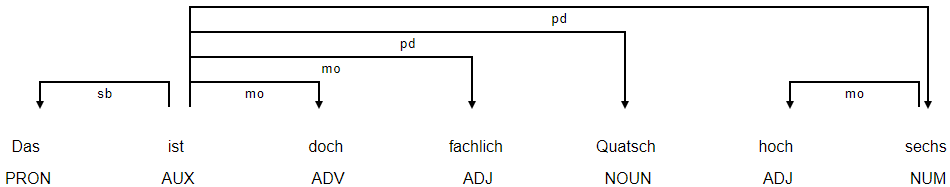
\includegraphics[width=1\textwidth]{chapters/04-Sentiment-Analyse/steffi.png}}
\caption{Visualisierung der Wortabhängigkeiten (Zitat von Steffi Lemke MdB, 208. Sitzung, 10.02.2021)}
\label{steffi}
\end{figure}

\subsection{Negations-Erkennung}
\label{neg-erkennung}
Negation, also Ablehnung, Verneinung oder Aufhebung, hat einen erheblichen Einfluss auf das Ergebnis und damit die Korrektheit der Sentimentanalyse, weshalb in dieser Arbeit ein besonderes Augenmerk auf ihre Erkennung gelegt wurde. 
In \textit{Negation Modeling for German Polarity Classification} \cite{g3_wieg} präsentieren Forscher der Universität des Saarlandes und des Leibniz-Institut für Deutsche Sprache hierfür einen regelbasierten Ansatz. 

Sie definieren unterschiedliche Negationstypen und ihre jeweilige Reichweite. 
So beeinflussen etwa negierende Adverbien oder Indefinitpronomen wie \textit{nie} den gesamten Satz, wohingegen das Partikel \textit{nicht} lediglich seinen Vorgänger negiert.  
Die Tabelle \ref{g3tab1} führt alle in dieser Arbeit implementierten Negationsregeln auf. 
Die Nutzung eines Abhängigkeitsbaumes, wie von \mintinline{latex}{spaCy} ermittelt, ist dabei unerlässlich. 
Denn wie schon im vorherigen Kapitel angesprochen, ist etwa mit dem Vorgänger eines Wortes nicht das in der Satzabfolge voranstehende Wort gemeint, sondern vielmehr der semantische Regent. 

\begin{table}[htbp]
\caption{Implementierte Negations-Regeln aus \cite{g3_wieg}}
\begin{center}
\begin{tabular}{| c | c | c |}
\hline
\textbf{Negationstyp} & \textbf{Reichweite} & \textbf{Beispielworte} \\ \hline
Partikel & Vorgänger (Regent) & nicht \\ \hline
Präpositionen & Nachfolger (Dependent) & ohne, gegen \\ \hline
Adverbien, & Satz & nie, kein, kaum \\
Indefinitpronomen &  &  \\ \hline
Nomen & Genitiv,& Abschaffung, \\
 & Präpositionalobjekt & Zerstörung \\ \hline
Verben & Objekt, Subjekt & enden, sinken, lindern \\
\hline
\end{tabular}
\label{g3tab1}
\end{center}
\end{table}

Angemerkt sei an dieser Stelle, dass es nicht möglich war, alle Regeln aus \cite{g3_wieg} zu implementieren, da der von den Forschern genutzte Dependency-Parser umfangreichere Ergebnisse liefert, als jener von \mintinline{latex}{spaCy}. 

Eine Liste mit Negationsworten und dem jeweiligen Negationstyp wurde \cite{g3_polcla} entnommen und ist ebenfalls über die Klasse \mintinline{latex}{Lexicon} zugreifbar. 
Die Klasse stellt ein \mintinline{latex}{Dictionary} bereit, in welchem die Schlüssel die Negationsworte und die Werte eine Liste der Reichweiten sind. 

Wenn in einem Text ein Negationswort auftritt, werden alle implementierten Regeln geprüft. 
Sollte es zu einem Treffer kommen, etwa wenn das Wort \textit{nicht} auftritt (siehe Abb. \ref{brandner}) und es einen Vorgänger gibt, werden alle Worte in Reichweite des Negationswortes negiert. 
Dies geschieht, indem für die jeweiligen Worte, welche wie in \ref{g3textv} beschrieben \mintinline{latex}{Token}-Objekte sind, ein eigenes Attribut mit der Bezeichnung \mintinline{latex}{negated} auf \mintinline{latex}{True} gesetzt wird. 
In der Polaritätsberechnung wird wortweise auf dieses Attribut geprüft und die Wort-Polarität bei einer Negierung mit -1 multipliziert. 

\begin{figure}[htb]
\centerline{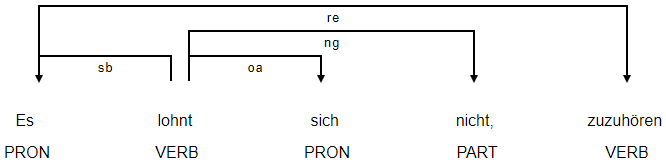
\includegraphics[width=1\textwidth]{chapters/04-Sentiment-Analyse/brandner.png}}
\caption{Beispielsatz mit Patikel-Negation (Zitat von Stephan Brandner MdB, 207. Sitzung, 29.01.2021)}
\label{brandner}
\end{figure}

\subsection{Verstärkungs-Erkennung}
\label{ver-erkennung}
Als \textit{Verstärker} werden sog. Gradpartikel (z.B. sehr, besonders, viel) verstanden, welche direkt vor Adjektiven oder Adverbien in einem Satz auftreten. 
Sie verstärken ihren Nachfolger, was wiederum in der Polaritätsberechnung berücksichtigt werden soll. 

Aus diesem Grund wird eine Liste mit verstärkenden Gradpartikeln, welche ebenfalls aus \cite{g3_polcla} bezogen werden, eingelesen und über die \mintinline{latex}{Lexicon} Klasse bereitgestellt. 

Ebenso wie in Kapitel \ref{neg-erkennung} bereits für die Negation beschrieben, wird ein eigenes Attribut zur Signalisierung einer Verstärkung definiert und im entsprechenden Fall auf True gesetzt. 
Bei der Polaritätsberechnung wird bei einer erkannten Verstärkung die Wort-Polarität mit 1,5 multipliziert \cite{g3_sentia}. 

In Abbildung \ref{hessel} wird ein Beispiel für das Auftreten eines verstärkenden Gradpartikels gegeben. 
Hier verstärkt das Wort \textit{sehr} das negative Wort \textit{spät}, womit die errechnete Polarität stärker negativ ausfällt als ohne die Verstärkungs-Erkennung. 

\begin{figure}[htb]
\centerline{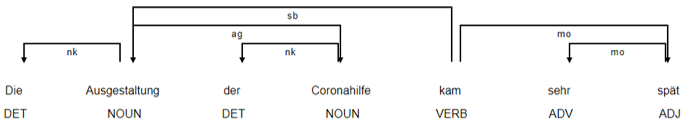
\includegraphics[width=1\textwidth]{chapters/04-Sentiment-Analyse/hessel.png}}
\caption{Beispielsatz mit Gradpartikel-Verstärkung (Zitat von Katja Hessel MdB, 206. Sitzung, 28.01.2021)}
\label{hessel}
\end{figure}

\subsection{Polaritätsberechnung}
\label{polberechnung}
Für die abschließende Berechnung der Polarität sind verschiedene Formeln denkbar. 
Sie sollten anhand von Textcharakteristika wie z.B. der Satz- oder Textlänge gewählt werden. 

Bei der Verwendung einer satzbasierten Polaritätsberechnung, bei welcher alle Polaritäten erst addiert und die Summe anschließend durch die Anzahl der Worte dividiert wird, kann ein unerwünschtes Phänomen auftreten: 
Längere Sätze erhaltenen ein stärker polarisiertes Ergebnis als vergleichbare kurze Sätze. 

Dies ist mit einer im Schnitt höheren Dichte an Worten mit Polaritäts-Wert in längeren Sätzen zu erklären. 
Um diesem Problem entgegen zu wirken, wurde in dieser Arbeit eine Min-Max-Skalierung (siehe Formeln 1 - 3) auf Dokumentebene implementiert \cite{g3_sentia}. 

Die Entscheidung, diese Normalisierung anhand der Länge des gesamten Textes durchzuführen, wurde aufgrund der Charakteristika der zu analysierenden Interaktionen getroffen. 
Denn diese bestehen zu einem überwiegenden Teil aus einem einzelnen Satz von jedoch sehr unterschiedlicher Länge. 

\begin{align}
p' &= \frac{ p + 1 }{ text.len + 1 } \text{ für p $>$ 0}\\
p' &= \frac{ p - 1 }{ text.len + 1 } \text{ für p $<$ 0}\\
p' &= p \text{ für p $=$ 0}
\end{align}

\section{Evaluierung}
\subsection{Sprache im Bundestag}
\label{sprachebundestag}
Während der Entwicklung dieser Arbeit und den regelmäßig angestellten Zwischentests wurde ersichtlich, dass sich die Sprache im Bundestag etwa von jener in sozialen Netzwerken oder Produktbewertungen unterschiedet. 
Ein Interaktionstext setzt sich sowohl aus einzelnen, langen und komplexe Sätze zusammen, als auch aus einzelnen Ausrufen wie \textit{\glqq eieiei!\grqq} zusammen. 

Aus diesem Grund wurde die in \ref{polberechnung} beschriebene Normalisierung verwendet, da herkömmliche Berechnungsformeln zunächst widersprüchliche Ergebnisse lieferten. 
Gleichzeitig verbesserte die manuelle Durchsicht der häufigsten 15.000 Worte und Anfertigung einer eigenen Bundestags-Wortliste das Ergebnis deutlich. 
Viele der regelmäßig in Bundestagssitzungen verwendeten Worte gehören zur \textit{Politik-Domäne} und treten deshalb nicht in den Quell-Wortlisten auf. 
Hier wird erwartet, dass eine noch umfangreichere Bundestags-Wortliste einen weiteren positiven Einfluss auf das Endergebnis hätte. 
Aus Zeit- sowie Kompetenzgründen wurde diese Liste jedoch nicht erweitert. 

\subsection{Ironie und Sarkasmus}
Ebenso wie die im vorherigen besprochene \textit{Politiksprache}, treten auch Ironie und Sarkasmus vermehrt in den Sitzungen des Bundestages auf. 
Einfach umrissen, handelt es sich dabei um ein Stilmittel, bei dem das Gegenteil vom Gesagten gemeint ist. 
Sarkasmus ist dabei eine verstärkte Form der Ironie und kann auch als ein Angriff verstanden werden. 

Selbst für den menschlichen Leser ist allein am geschriebenen Text nicht immer ersichtlich, ob eine Aussage ironisch gemeint ist. 
Vielmehr wird für die richtige Deutung die Stimmlage, Gestik und Mimik der sprechenden Person benötigt. 

Ironie und Sarkasmus könne also erst recht nicht mit dem in dieser Arbeit verwendeten Wortlisten-Ansatz erkannt werden, womit ein unbekannter Teil der Interaktionen im Ergebnis die falsche Polarität besitzt. 
Gleichwohl gibt es Ansätze aus dem Bereich des maschinellen Lernens, welche dieses Problem behandeln. 
Jedoch setzen diese einen entsprechend annotierten Korpus vorraus und stammen zudem aus dem Bereich der sozialen Netzwerke, in welchen etwa mit \textit{Hashtags} die Ironie bereits vom Autor markiert wurde. 

\subsection{Fazit}
Trotzt der soeben beschriebenen Fehlerquellen, wurde dennoch ein gelungenes Ergebnis erzielt: 
Es wurde ein solider und erweiterbarer Algorithmus zur Sentimentananlyse von Texten geschaffen, welcher auf den bekanntesten Bibliotheken und Techniken der Textverarbeitung beruht. 
Dieser kann als Basis für weitere Anstrengungen bei der Sentimentanalyse von politischen Texten dienen. 

Eine Deutung der bisherigen Ergebnisse durch Politikwissenschaftler oder anderweitig in diesem Bereich kompetente Personen wird dabei empfohlen, um die beschriebenen Schwachstellen entsprechend zu behandeln oder neue zu identifizieren. 

Der Programmcode ist zudem vollständig und abgesichert in die Projektpipeline eingebunden. 
Er erweitert seine Ergebnis-Datenbank automatisch um neue Sitzungen und benachrichtigt anschließend nachfolgende Gruppen. 

\section{Grundlagen}\label{sec:07_02_grundlagen}
\section{Anforderungsanalyse und Konzept}\label{sec:08_03_anforderungen_konzept}


\section{Zusammenfassung und Ausblick}\label{sec:07_05_zusammenfassung}

\chapter{Benutzeroberfläche}
Die Gruppe 8 hat sich mit der Erstellung der Benutzeroberfläche beschäftigt. Das Team bestand aus den vier Studenten, Amanda Joelle Dzukou Kom, Steven Mi, Tilman Möller und Oliver Kütemeier. Die Implementation des Projektes wurde in enger Zusammenarbeit der Studenten umgesetzt, um eine gleichmäßige Verteilung der Kompetenzen zu sichern. 
\section{Einleitung}
Der Begriff \textit{Sentiment} stammt vom lateinischen Wort \textit{sentimentum} ab und bedeutet Empfindung oder Stimmung. 
In der Sentimentanalyse geht es um die Bestimmung eben jener Stimmung einer Meinungsäußerung. 
Anwendung findet sie etwa bei Produktbewertungen oder Beiträgen in sozialen Netzwerken. 
Die Stimmung wird durch die sog. Polarität beschrieben und kann positiv, negativ oder neutral ausfallen. 
Im Text-Mining wird sie im Intervall $\interval{-1}{1} = \{x \in \mathbb{R} | -1 \leq x \leq 1\}$ angegeben, wobei -1 sehr negativ, 1 sehr positiv und 0 neutral bedeuten. 

Grundlegend ist die maschinelle Sentimentanalyse entweder Wortlisten- oder Modell-basiert. 
Der Wortlisten-Ansatz kann als eine Sammlung von Worten und ihrer Polaritäten verstanden werden, anhand welcher die Stimmung berechnet wird. 
Dieser Ansatz wird weiter im Kapitel \ref{wortliste} beschrieben, da er in dieser Arbeit verwendet wurde. 

Bei der Modell-basierten Sentimentanalyse wird ein annotierter Satz-Korpus für das Trainieren einer künstlichen Intelligenz vorausgesetzt. 
Etwa für Twitter-Beiträge stehen solche Korpusse oder auch bereits trainierte Modelle zur Verfügung. 
Jedoch ist bei der Verwendung zur Analyse der Sitzungsprotokolle des Bundestages nicht mit zufriedenstellenden Ergebnissen zu rechnen, da sich verwendete Worte und Text- bzw. Satzbau zwischen diesen Domänen deutlich unterscheiden. 
Eine weitere Erläuterung zur Sprache im Bundestag wird in Kapitel \ref{sprachebundestag} gegeben. 

Ebenfalls werden die Komponenten zur Teilnahme an der Verarbeitungspipeline des Gesamtprojektes im nachfolgenden Kapitel \ref{g3daten} beschrieben. 

\section{Datenaustausch}
\label{g3daten}
\subsection{Datenimport}
Für das Erhalten von Daten wurde eine Methode implementiert, welche durch Angabe einer Sitzungs-ID die entsprechende Sitzung vom REST-API von Gruppe 2 abfragen kann. 
Diese Methode gibt jede Sitzung weiter an die in Kapitel \ref{g3textv} beschriebene Textverarbeitung und das Ergebnis schließlich an den in Kapitel \ref{g3export} beschriebenen Export-Code. 

Die Methode wird für zwei Fälle verwendet: 
Beim Normalfall sendet die Gruppe 2 eine Benachrichtigung mit einer Liste aller neuen Sitzungs-IDs an das REST-API im Code dieser Arbeit. 
Das REST-API wurde mit der Bibliothek \mintinline{latex}{Flask} \cite{g3_flask} entwickelt und besteht aus einer POST-Schnittstelle, welche auf dem von der HTW bereitgestelltem Server unter \textit{/notify} erreichbar ist. 

Das API wurde unter Zuhilfenahme von \mintinline{latex}{Flask.Blueprints} \cite{g3_flaskbp} entwickelt und wird von einem \mintinline{latex}{Waitress}-Webserver \cite{g3_waitress} bereitgestellt. 
Für jede Anfrage wird geprüft, ob Content-Type und Payload dem erwarteten JSON-Daten entsprechen. 
Sollte dies nicht der Fall sein, wird eine entsprechende Rückmeldung an den Sender zurückgegeben. 
Für jede erhaltene Sitzungs-ID wird die eingangs beschriebene Methode aufgerufen. 

Der zweite Fall wurde vor allem im Rahmen der voranschreitenden Entwicklung bei den in der Projektpipeline voranstehenden Gruppen verwendet. 
Statt auf eine Benachrichtigung zum Anstoßen des Datenimports zu warten, werden stattdessen alle Sitzungs-IDs vom REST-API der Gruppe 2 abgefragt und jede Sitzung vollständig neu importiert. 
Dieses Vorgehen hat den Vorteil, dass eventuell durch Arbeit am Code verpasste Benachrichtigungen nachgeholt werden und gleichzeitig Änderungen an den Daten übernommen werden können. 

\subsection{Datenexport}
\label{g3export}
Statt Arbeit in ein umfangreiches REST-API für die nachfolgenden Gruppen zu stecken, wurde für diese Arbeit ein reiner MongoDB-Ansatz verwendet. 
Auf dem zur Verfügung stehenden HTW-Server wurde dafür eine MongoDB Instanz aufgesetzt, welche nur aus dem HTW-Netz erreichbar und zudem nur mit Authentifizierung zugreifbar ist. 
Jede Sitzung ist hier als eine eigene Collection persistiert. 
Sobald neue Sitzungen importiert und verarbeitet wurden, werden diese zunächst mit dem MongoDB-Treiber \mintinline{latex}{PyMongo} \cite{g3_mongodb} in die Datenbank geschrieben. 
Anschließend werden die nachfolgenden Gruppen mit einem POST and die jeweilige REST-Schnittstelle benachrichtigt, dass neue Daten vorliegen. 
Diese greifen dann mit den zuvor versendeten Zugangsdaten direkt auf die Datenbank zu. 

Mit diesem Vorgehen konnte die Komplexität beim Zugriff auf die Ergebnis-Daten gesenkt werden, da es für nahezu alle gängigen Programmiersprachen einen intuitiven MongoDB-Treiber gibt. 

\section{Wortliste}
\label{wortliste}
Wie bereits in der Einleitung beschrieben, handelt es sich bei Wortlisten in der Sentimentanalyse um eine Liste von Worten und ihrer jeweiligen Polarität. 
Bei der Analyse eines Textes wird wortweise ein Abgleich mit dieser Liste durchgeführt und die Wort-Polarität bei einer Übereinstimmung für die Berechnung des Sentiments verwendet. 
Unterschiedliche Berechnungsformeln sind dabei denkbar und werden in Kapitel \ref{polberechnung} weiter besprochen. 
Für diese Arbeit wurden Wortlisten verschiedener Institutionen kombiniert und anschließend mit Synonymen erweitert. 
Ebenfalls wurde eine eigene Bundestags-Wortliste erstellt. 

Die Interest Group on German Sentiment Analysis (IGGSA) stellt eine umfangreiche Liste an Publikationen und Ressourcen zu Sentimentanalysen in der deutschen Sprache zur Verfügung \cite{g3_iggsa}. 
Hier wurden alle Referenzen auf die in dieser Arbeit verwendeten Quell-Wortlisten gesammelt. 
Für die Zusammenführung dieser Wortlisten wurden zunächst zwei Herangehensweisen evaluiert: 
Zum einen war die Erstellung eines eigenständigen Codes denkbar, welcher einmalig die Daten aus allen Quellen einliest, zusammenfasst und eine Ergebnis-Datei ausgibt. 
Diese Datei wäre eine Ressource für den eigentlichen Analyse-Code. 
Zum anderen könnte die soeben beschriebene Funktionalität jedoch auch direkt im Analyse-Code integriert und bei jedem Programmstart ausgeführt werden. 
Die kombinierte Wortliste würde somit nicht auf die Festplatte geschrieben, sondern im Arbeitsspeicher verbleiben, solange der Analyse-Code läuft. 
Wenngleich der zuerst beschriebene Ansatz offensichtlich weniger Rechenzeitaufwändig ist, wurde für diese Arbeit der zweite Ansatz gewählt. 
Dies wird vor allem mit Rechtsunsicherheiten bei der Arbeit mit den verschiedenen Lizenzen der Quelldateien begründet. 
Gleichzeitig arbeitet der Analyse-Code damit jederzeit mit dem aktuellen Stand der Quell-Wortlisten. 
Das Aufbauen der Wortliste dauert wenige Minuten. 

Für diese Arbeit wurden die folgenden Quell-Wortlisten verwendet: 

\begin{itemize}
\item \textit{SentimentWortschatz} (SentiWS) aus \glqq SentiWS - a Publicly Available German-language Resource for Sentiment Analysis\grqq (Universität Leipzig) \cite{g3_sentiws}
\item \textit{Multi-Domain Sentiment Lexicon for German} (Hochschule Darmstadt) \cite{g3_opm}
\item \textit{German Polarity Lexicon} aus \glqq Evaluation and extension of a polarity lexicon for German\grqq (Universität Zürich) \cite{g3_polcla}
\item \textit{morphcomp} aus \glqq Evaluating the morphological compositionality of pola-rity\grqq (Leibniz-Institut für Deutsche Sprache, Universität des Saarlandes) \cite{g3_morphcomp}
\end{itemize}

Aus diesen Quellen ergibt sich eine Wortliste mit etwa 14.000 einzigartigen Worten. 
Die Worte werden dabei mit der in Kapitel \ref{g3textv} beschriebenen Textverarbeitungspipeline lemmatisiert, also auf die Grundform zurückgeführt. 
Bei Überschneidungen wird ein Mittelwert über alle Polaritäts-Werte eines Wortes gebildet. 

Mithilfe des \textit{Open German WordNet} (OdeNet) \cite{g3_odenet} werden zu jedem Wort Synonyme gesammelt und ebenfalls der Wortliste hinzugefügt. 
Der Zugriff auf OdeNet geschieht dabei mit der python Bibliothek \mintinline{latex}{WN} \cite{g3_wn}. 
Die Verwendung dieser Bibliothek ist trivial, weshalb an dieser Stelle keine weitere Erläuterung gegeben wird. 
Die Wortliste wird durch das Hinzufügen von Synonymen um weitere rund 2.000 Worte erweitert. 

Wie bereits in der Einleitung erwähnt, wurde zudem eine eigene Bundes-tags-Wortliste erstellt. 
Hierzu wurden die 15.000 am häufigsten in den Sitzungsprotokollen vorkommenden Worte erfasst und analysiert. 
Dabei wurden jedoch nur jene Worte betrachtet, welche nicht bereits in der kombinierten Wortliste vorkommen. 
Ausgewählt wurden nur eindeutig positive oder negative Worte wie \textit{angemessen}, \textit{Bullshit}, \textit{Fehlentscheidung}, \textit{Milchmädchenrechnung}, \textit{Realitätsverweigerung}, \textit{Totalausfall} oder \textit{Verunglimpfung}. 
Insgesamt umfasst die Bundestags-Wortliste 217 Worte. 

Im Code wird der Zugriff auf die Wortliste mit der zentralen Klasse \mintinline{latex}{Lexicon} realisiert. 
Bei der Instanziierung der Klasse werden, wie im Vorherigen beschrieben, alle Wortlisten gesammelt, zusammengeführt und erweitert. 
Anschließend stellt die Klasse ein \mintinline{latex}{Dictionary} bereit, in welchem die Schlüssel die Worte und die Werte die Wort-Polarität angeben. 

\section{Textverarbeitung}
\label{g3textv}
Für die Textverarbeitung nutzt der Code dieser Arbeit vollständig die Funktionalitäten und Strukturen von \mintinline{latex}{spaCy} \cite{g3_spacy}. 
Die \mintinline{latex}{spaCy} Bibliothek stellt eine Textverarbeitungspipeline bereit, welche mithilfe eines vortrainierten Modells funktioniert. 
Für die deutsche Sprache wurde ein solches Modell mit dem TIGER Korpus der Universität Stuttgart trainiert. 
Der Korpus umfasst ca. 50.000 Sätze aus Texten der Frankfurter Rundschau. 
Die \mintinline{latex}{spaCy}-Pipeline besteht aus den folgenden Komponenten: 

\begin{itemize}
\item Tokenisierung (Text- und Satzzerteilung)
\item POS-Tagging (Wortartenerkennung)
\item Dependency-Parsing (Wortabhängigkeitenerkennung)
\item Lemmatisierung (Wortgrundformermittlung)
\item Entity-Recognition (Eigennamenerkennung)
\end{itemize}

Das Ergebnis der Pipeline ist ein \mintinline{latex}{Doc}-Objekt, welches das Ergebnis des gesamten in die Pipeline gegebenen Textes umfasst. 
Einzelne Sätze innerhalb des \mintinline{latex}{Doc}-Objektes werden mit \mintinline{latex}{Span}-Objekten beschrieben und einzelne Worte mit \mintinline{latex}{Token}-Objekten. 
Die Objekttypen besitzen jeweils eigene Methoden und Erweiterungsmöglichkeiten in Form von sog. \textit{extension attributes}. 

Sehr einfach und gleichzeitig umfangreich kann die \mintinline{latex}{spaCy}-Pipeline an die eigenen Bedürfnisse angepasst werden. 
So wurde die Berechnung des Sentiments eines Textes direkt an die Komponenten der Standart-Pipeline angehängt. 
Logisch unterteilt sich diese in die Komponenten:

\begin{itemize}
\item Negations-Erkennung (siehe \ref{neg-erkennung})
\item Verstärkungs-Erkennung (siehe \ref{ver-erkennung})
\item Polaritätsberechnung (siehe \ref{polberechnung})
\end{itemize}

Basis für das nachfolgende Kapitel \ref{neg-erkennung} ist dabei das Ergebnis des Depen-dency-Parsers von \mintinline{latex}{spaCy}. 
Dieser bestimmt die Abhängigkeiten zwischen den einzelnen Elementen eines Satzes. 
Diese Funktion gehört dem Themenbereich der Dependenzgrammatik an, in welcher gerichtete Beziehungen zwischen den Worten eines Satzes beschreibt werden. 
Ein Wort kann einen Vorgänger (Regent) und mehrere Nachfolger (Dependenten) besitzen. 
Die Gesamtheit der Beziehungen eines Satzes wird auch Abhängigkeitsbaum genannt. 

Zur Verdeutlichung soll die Abbildung \ref{steffi} dienen, welche mithilfe von \mintinline{latex}{spaCy.displaCy} erstellt wurde. 
Zu sehen ist hier der Abhängigkeitsbaum des Satzes \textit{\glqq Das ist doch fachlich Quatsch hoch sechs!\grqq}. 
An den gerichteten Kanten befindet sich die Angabe des Satzgliedes, unterhalb der Worte die Angabe der Wortart. 

\begin{figure}[htb]
\centerline{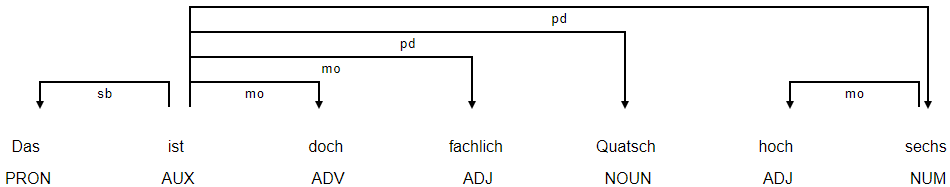
\includegraphics[width=1\textwidth]{chapters/04-Sentiment-Analyse/steffi.png}}
\caption{Visualisierung der Wortabhängigkeiten (Zitat von Steffi Lemke MdB, 208. Sitzung, 10.02.2021)}
\label{steffi}
\end{figure}

\subsection{Negations-Erkennung}
\label{neg-erkennung}
Negation, also Ablehnung, Verneinung oder Aufhebung, hat einen erheblichen Einfluss auf das Ergebnis und damit die Korrektheit der Sentimentanalyse, weshalb in dieser Arbeit ein besonderes Augenmerk auf ihre Erkennung gelegt wurde. 
In \textit{Negation Modeling for German Polarity Classification} \cite{g3_wieg} präsentieren Forscher der Universität des Saarlandes und des Leibniz-Institut für Deutsche Sprache hierfür einen regelbasierten Ansatz. 

Sie definieren unterschiedliche Negationstypen und ihre jeweilige Reichweite. 
So beeinflussen etwa negierende Adverbien oder Indefinitpronomen wie \textit{nie} den gesamten Satz, wohingegen das Partikel \textit{nicht} lediglich seinen Vorgänger negiert.  
Die Tabelle \ref{g3tab1} führt alle in dieser Arbeit implementierten Negationsregeln auf. 
Die Nutzung eines Abhängigkeitsbaumes, wie von \mintinline{latex}{spaCy} ermittelt, ist dabei unerlässlich. 
Denn wie schon im vorherigen Kapitel angesprochen, ist etwa mit dem Vorgänger eines Wortes nicht das in der Satzabfolge voranstehende Wort gemeint, sondern vielmehr der semantische Regent. 

\begin{table}[htbp]
\caption{Implementierte Negations-Regeln aus \cite{g3_wieg}}
\begin{center}
\begin{tabular}{| c | c | c |}
\hline
\textbf{Negationstyp} & \textbf{Reichweite} & \textbf{Beispielworte} \\ \hline
Partikel & Vorgänger (Regent) & nicht \\ \hline
Präpositionen & Nachfolger (Dependent) & ohne, gegen \\ \hline
Adverbien, & Satz & nie, kein, kaum \\
Indefinitpronomen &  &  \\ \hline
Nomen & Genitiv,& Abschaffung, \\
 & Präpositionalobjekt & Zerstörung \\ \hline
Verben & Objekt, Subjekt & enden, sinken, lindern \\
\hline
\end{tabular}
\label{g3tab1}
\end{center}
\end{table}

Angemerkt sei an dieser Stelle, dass es nicht möglich war, alle Regeln aus \cite{g3_wieg} zu implementieren, da der von den Forschern genutzte Dependency-Parser umfangreichere Ergebnisse liefert, als jener von \mintinline{latex}{spaCy}. 

Eine Liste mit Negationsworten und dem jeweiligen Negationstyp wurde \cite{g3_polcla} entnommen und ist ebenfalls über die Klasse \mintinline{latex}{Lexicon} zugreifbar. 
Die Klasse stellt ein \mintinline{latex}{Dictionary} bereit, in welchem die Schlüssel die Negationsworte und die Werte eine Liste der Reichweiten sind. 

Wenn in einem Text ein Negationswort auftritt, werden alle implementierten Regeln geprüft. 
Sollte es zu einem Treffer kommen, etwa wenn das Wort \textit{nicht} auftritt (siehe Abb. \ref{brandner}) und es einen Vorgänger gibt, werden alle Worte in Reichweite des Negationswortes negiert. 
Dies geschieht, indem für die jeweiligen Worte, welche wie in \ref{g3textv} beschrieben \mintinline{latex}{Token}-Objekte sind, ein eigenes Attribut mit der Bezeichnung \mintinline{latex}{negated} auf \mintinline{latex}{True} gesetzt wird. 
In der Polaritätsberechnung wird wortweise auf dieses Attribut geprüft und die Wort-Polarität bei einer Negierung mit -1 multipliziert. 

\begin{figure}[htb]
\centerline{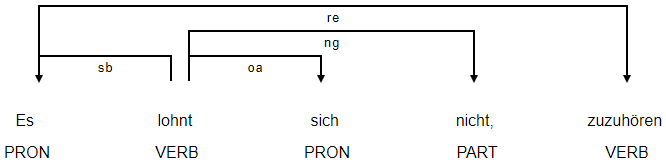
\includegraphics[width=1\textwidth]{chapters/04-Sentiment-Analyse/brandner.png}}
\caption{Beispielsatz mit Patikel-Negation (Zitat von Stephan Brandner MdB, 207. Sitzung, 29.01.2021)}
\label{brandner}
\end{figure}

\subsection{Verstärkungs-Erkennung}
\label{ver-erkennung}
Als \textit{Verstärker} werden sog. Gradpartikel (z.B. sehr, besonders, viel) verstanden, welche direkt vor Adjektiven oder Adverbien in einem Satz auftreten. 
Sie verstärken ihren Nachfolger, was wiederum in der Polaritätsberechnung berücksichtigt werden soll. 

Aus diesem Grund wird eine Liste mit verstärkenden Gradpartikeln, welche ebenfalls aus \cite{g3_polcla} bezogen werden, eingelesen und über die \mintinline{latex}{Lexicon} Klasse bereitgestellt. 

Ebenso wie in Kapitel \ref{neg-erkennung} bereits für die Negation beschrieben, wird ein eigenes Attribut zur Signalisierung einer Verstärkung definiert und im entsprechenden Fall auf True gesetzt. 
Bei der Polaritätsberechnung wird bei einer erkannten Verstärkung die Wort-Polarität mit 1,5 multipliziert \cite{g3_sentia}. 

In Abbildung \ref{hessel} wird ein Beispiel für das Auftreten eines verstärkenden Gradpartikels gegeben. 
Hier verstärkt das Wort \textit{sehr} das negative Wort \textit{spät}, womit die errechnete Polarität stärker negativ ausfällt als ohne die Verstärkungs-Erkennung. 

\begin{figure}[htb]
\centerline{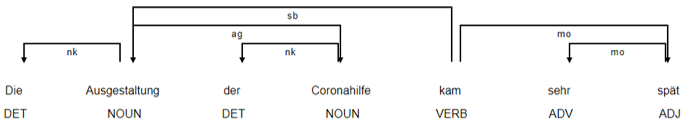
\includegraphics[width=1\textwidth]{chapters/04-Sentiment-Analyse/hessel.png}}
\caption{Beispielsatz mit Gradpartikel-Verstärkung (Zitat von Katja Hessel MdB, 206. Sitzung, 28.01.2021)}
\label{hessel}
\end{figure}

\subsection{Polaritätsberechnung}
\label{polberechnung}
Für die abschließende Berechnung der Polarität sind verschiedene Formeln denkbar. 
Sie sollten anhand von Textcharakteristika wie z.B. der Satz- oder Textlänge gewählt werden. 

Bei der Verwendung einer satzbasierten Polaritätsberechnung, bei welcher alle Polaritäten erst addiert und die Summe anschließend durch die Anzahl der Worte dividiert wird, kann ein unerwünschtes Phänomen auftreten: 
Längere Sätze erhaltenen ein stärker polarisiertes Ergebnis als vergleichbare kurze Sätze. 

Dies ist mit einer im Schnitt höheren Dichte an Worten mit Polaritäts-Wert in längeren Sätzen zu erklären. 
Um diesem Problem entgegen zu wirken, wurde in dieser Arbeit eine Min-Max-Skalierung (siehe Formeln 1 - 3) auf Dokumentebene implementiert \cite{g3_sentia}. 

Die Entscheidung, diese Normalisierung anhand der Länge des gesamten Textes durchzuführen, wurde aufgrund der Charakteristika der zu analysierenden Interaktionen getroffen. 
Denn diese bestehen zu einem überwiegenden Teil aus einem einzelnen Satz von jedoch sehr unterschiedlicher Länge. 

\begin{align}
p' &= \frac{ p + 1 }{ text.len + 1 } \text{ für p $>$ 0}\\
p' &= \frac{ p - 1 }{ text.len + 1 } \text{ für p $<$ 0}\\
p' &= p \text{ für p $=$ 0}
\end{align}

\section{Evaluierung}
\subsection{Sprache im Bundestag}
\label{sprachebundestag}
Während der Entwicklung dieser Arbeit und den regelmäßig angestellten Zwischentests wurde ersichtlich, dass sich die Sprache im Bundestag etwa von jener in sozialen Netzwerken oder Produktbewertungen unterschiedet. 
Ein Interaktionstext setzt sich sowohl aus einzelnen, langen und komplexe Sätze zusammen, als auch aus einzelnen Ausrufen wie \textit{\glqq eieiei!\grqq} zusammen. 

Aus diesem Grund wurde die in \ref{polberechnung} beschriebene Normalisierung verwendet, da herkömmliche Berechnungsformeln zunächst widersprüchliche Ergebnisse lieferten. 
Gleichzeitig verbesserte die manuelle Durchsicht der häufigsten 15.000 Worte und Anfertigung einer eigenen Bundestags-Wortliste das Ergebnis deutlich. 
Viele der regelmäßig in Bundestagssitzungen verwendeten Worte gehören zur \textit{Politik-Domäne} und treten deshalb nicht in den Quell-Wortlisten auf. 
Hier wird erwartet, dass eine noch umfangreichere Bundestags-Wortliste einen weiteren positiven Einfluss auf das Endergebnis hätte. 
Aus Zeit- sowie Kompetenzgründen wurde diese Liste jedoch nicht erweitert. 

\subsection{Ironie und Sarkasmus}
Ebenso wie die im vorherigen besprochene \textit{Politiksprache}, treten auch Ironie und Sarkasmus vermehrt in den Sitzungen des Bundestages auf. 
Einfach umrissen, handelt es sich dabei um ein Stilmittel, bei dem das Gegenteil vom Gesagten gemeint ist. 
Sarkasmus ist dabei eine verstärkte Form der Ironie und kann auch als ein Angriff verstanden werden. 

Selbst für den menschlichen Leser ist allein am geschriebenen Text nicht immer ersichtlich, ob eine Aussage ironisch gemeint ist. 
Vielmehr wird für die richtige Deutung die Stimmlage, Gestik und Mimik der sprechenden Person benötigt. 

Ironie und Sarkasmus könne also erst recht nicht mit dem in dieser Arbeit verwendeten Wortlisten-Ansatz erkannt werden, womit ein unbekannter Teil der Interaktionen im Ergebnis die falsche Polarität besitzt. 
Gleichwohl gibt es Ansätze aus dem Bereich des maschinellen Lernens, welche dieses Problem behandeln. 
Jedoch setzen diese einen entsprechend annotierten Korpus vorraus und stammen zudem aus dem Bereich der sozialen Netzwerke, in welchen etwa mit \textit{Hashtags} die Ironie bereits vom Autor markiert wurde. 

\subsection{Fazit}
Trotzt der soeben beschriebenen Fehlerquellen, wurde dennoch ein gelungenes Ergebnis erzielt: 
Es wurde ein solider und erweiterbarer Algorithmus zur Sentimentananlyse von Texten geschaffen, welcher auf den bekanntesten Bibliotheken und Techniken der Textverarbeitung beruht. 
Dieser kann als Basis für weitere Anstrengungen bei der Sentimentanalyse von politischen Texten dienen. 

Eine Deutung der bisherigen Ergebnisse durch Politikwissenschaftler oder anderweitig in diesem Bereich kompetente Personen wird dabei empfohlen, um die beschriebenen Schwachstellen entsprechend zu behandeln oder neue zu identifizieren. 

Der Programmcode ist zudem vollständig und abgesichert in die Projektpipeline eingebunden. 
Er erweitert seine Ergebnis-Datenbank automatisch um neue Sitzungen und benachrichtigt anschließend nachfolgende Gruppen. 

\section{Auswahl des Frameworks}%\label{sec:08_02_Auswahl-des-Frameworks}
Bei der Implementation des Frontends bestand der erste Schritt in der Auswahl des Frameworks. Die drei betrachteten Kandidaten waren Vue.js, Angular und React.

\begin{figure}[hbt!]%
  \centering
  \subfigure{
  
\includegraphics[width=3cm]{images/08-Benutzeroberfläche/08-Angular_logo.png}
  }%
  \qquad
  \subfigure{
  
\includegraphics[width=3cm]{images/08-Benutzeroberfläche/08-Vue_logo.png}
  }%
  \qquad
  \subfigure{
\includegraphics[width=4cm]{images/08-Benutzeroberfläche/08-react_logo.png}}%
  \caption{Logos der zur Auswahl stehenden Frameworks}%
\end{figure}

Nach erster Recherche wurde klar, dass alle Frameworks in der Lage sind moderne und stabile Webseiten zu erstellen. Sie unterstützen alle diverse Bibliotheken zur Visualisierung und bieten die Funktionalitäten die geplanten Inhalte umzusetzen. Da die drei Frameworks die technischen Anforderungen gleichmäßig erfüllen, konnten wir persönliche Kriterien aufstellen um eine Entscheidung zu treffen. 
Das erste Kriterium bestand in der aktuellen Nachfrage in der Wirtschaft. Dazu haben wir die Menge der Suchanfragen nach dem jeweiligen Skill in unterschiedlichen Bereichen untersucht. Angefangen haben wir mit den Jobbörsen und Business Social Networks.

\begin{figure}[hbt!]%
  \centering
  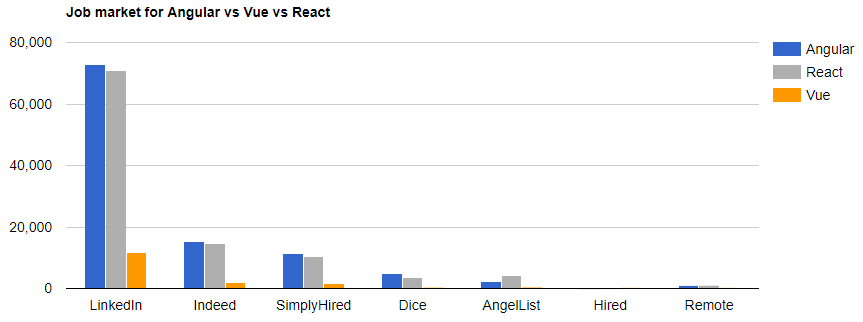
\includegraphics[width=14cm]{images/08-Benutzeroberfläche/08-jobbörsen-anfragen.PNG}
  \caption{Vergleich der Suchanfragen in Jobbörsen und Business Social Networks}%
\end{figure}

Hier ist klar, dass die Industrie mehr an den Frameworks React und Angular interessiert ist. Um die allgemeine Meinung besser einschätzen zu können haben wir die Google Trending Suchanfragen der verglichen. 

\begin{figure}[hbt!]%
  \centering
  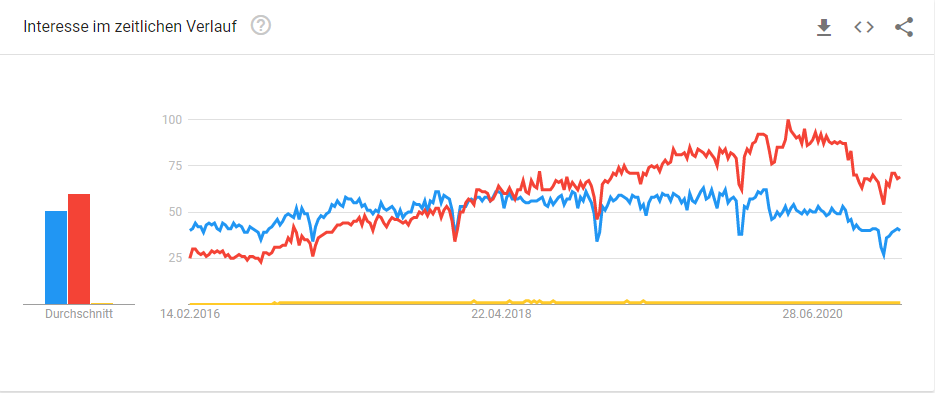
\includegraphics[width=14cm]{images/08-Benutzeroberfläche/08-google_trending.PNG}
  \caption{Vergleich der Google Trending Suchwörter}%
\end{figure}

Auch hier stehen Angular und React weit vor den Anfragen von, sodass wir uns zwischen diesen beiden entscheiden mussten. Als letztes Kriterium haben wir die aktuellen Github Statistiken der Frameworks verglichen um einen Eindruck für die Community und dessen Aktivität zu erhalten.

\begin{figure}[hbt!]%
\centering
  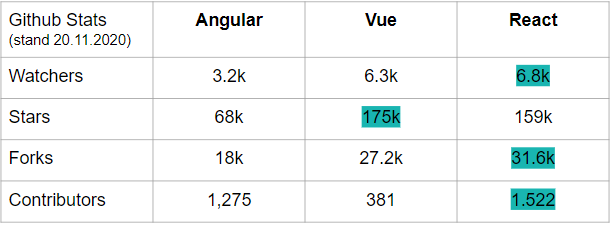
\includegraphics[width=14cm]{images/08-Benutzeroberfläche/08-github_stats.PNG}
  \caption{Vergleich der Github Statistiken der Frameworks}%
\end{figure}

Unter Berücksichtigung aller Kriterien haben wir uns für die Entwicklung der Website mit React entschieden.
\section{Infrastruktur}\label{sec:08_03_Infrastruktur}
Die Infrastruktur, welche unser Team zum verwalten des Quellcodes und zum bereitstellen der Webseite genutzt hat, war zum einen an die Absprachen der Studentengruppe und zum anderen an die Vorgaben der Hochschule gebunden. In Abstimmung mit allen Studenten wurde sich dazu entschieden, den Quellcode in Github zu verwalten. Die Bereitstellung erfolgte darüber hinaus über die Server der HTW Berlin, auf denen wir eine Virtuelle Maschine zur Verfügung gestellt bekommen haben.

\subsection{Quellcode Verwaltung}
Innerhalb der Github Organisation "Sentiments-of-Bundestag" haben wir das Git Repository "frontend\_sentiment" angelegt. Wir haben mithilfe der von Github eingeführten Issues eine Schnittstelle zum Kommunizieren von Problemen angelegt, die von den anderen Gruppen genutzt werden konnte. Über die Readme des Projekts haben wir alle wichtigen Befehle und Hilfestellungen zur Nutzung der Anwendung dokumentiert.
Durch integrieren eines Linters in den Build-Prozess der Anwendung konnten wir als Gruppe feste Quellcode-Formatierungs-Regeln definieren und befolgen um Clean Code zu implementieren. Als zusätzliche Regelung zur Unterbindung von Problemen beim Programmieren haben wir in Branches gearbeitet und bei Änderungen am Quellcode Rücksprache im Team gehalten. 

\subsection{Bereitstellung}
Bei der Bereitstellung der Anwendung haben wir die Serverkapazitäten der HTW Berlin genutzt. Uns wurde eine virtuelle Maschine zur Verfügung gestellt. Auf dieser mussten zunächst die Zugriffsregeln der Firewall angepasst werden um den Zugriff auf feste Ports, von außerhalb des HTW Netzwerks, zuzulassen. Außerdem mussten Git und Node.js installiert werden. Git wurde benötigt um den Quellcode aus dem Repository bei Änderungen herunterzuladen. Node.js wurde als Server zur Bereitstellung der React Anwendung benutzt.
\section{Design Thinking}\label{sec:08_04_Design_Thinking}
Beim Gestalten der Benutzeroberfläche haben wir uns an den sechs Phasen des von Tim Browns erfundenen Design Thinking Prozess orientiert. 

\begin{figure}[hbt!]
    \centering
    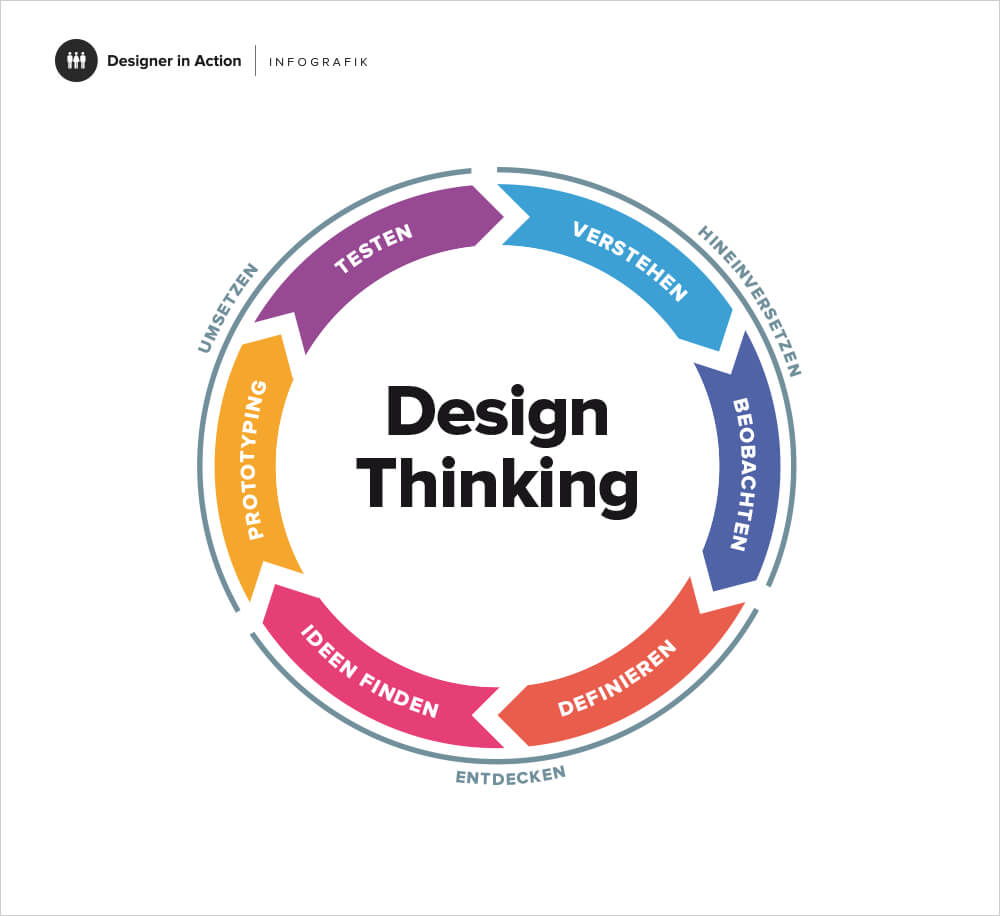
\includegraphics[width=14cm]{images/08-Benutzeroberfläche/08-Design Thinking.png}
    \caption{Ablauf des Design Thinking Prozess}
\end{figure}

Dieser Prozess wird im Online Artikel "Was ist Design Thinking?"\cite{DeTh} gut beschrieben. 
In diesem Projekt standen wir zunächst vor dem Problem, dass wir die Daten und fest definierten Schnittstellen erst im letzten drittel des Semesters vorliegen hatten. Vorher haben wir uns mit der Auswahl der Graphen- und Diagrammtypen beschäftigt. Wir haben Prototypen entwickelt und diese in regelmäßigen Abständen mit der Studentengruppe geteilt und Rückmeldungen gesammelt, welch in den Design Prozess eingeflossen sind. Mit den Rückmeldungen der Gruppe konnten wir unseren Prototypen verbessern, Teile umgestalten Beschreibungen anpassen oder Bereiche entfernen.
Die erste Iteration bestand in der Vorbereitung der Planungspräsentation unserer Gruppe. Bis zu diesem Zeitpunkt haben wir Ideen gesammelt, wie die angekündigten Daten in Diagrammen und für Benutzer*innen verständlich aufbereitet werden können. In einem Prototypen haben wir vier unterschiedliche Diagramme vorbereitet.

\begin{figure}[hbt!]%
    \centering
    \begin{subfigure}
        \centering
        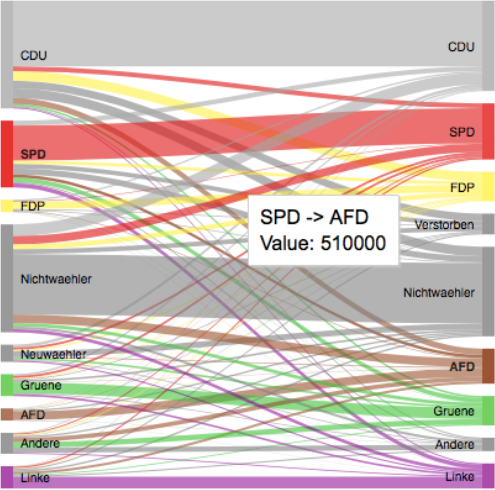
\includegraphics[width=5cm]{images/08-Benutzeroberfläche/08-flowchart.PNG}
    \end{subfigure}
    \qquad
    \begin{subfigure}
         \centering
         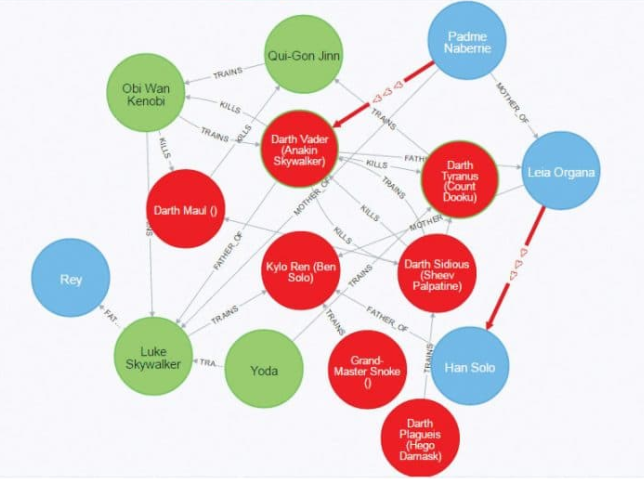
\includegraphics[width=5cm]{images/08-Benutzeroberfläche/08-Graphen.PNG}
    \end{subfigure}
    \qquad
    \begin{subfigure}
         \centering
        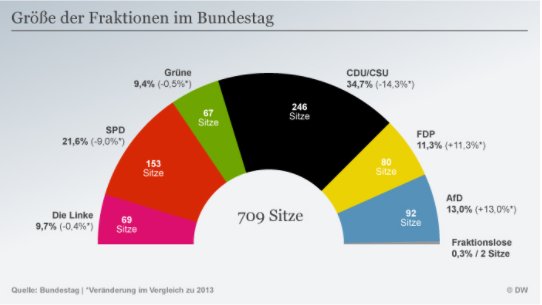
\includegraphics[width=5cm]{images/08-Benutzeroberfläche/08-Zusammensetzung_bundestag.PNG}
  \end{subfigure}
  \qquad
  \begin{subfigure}
        \centering
        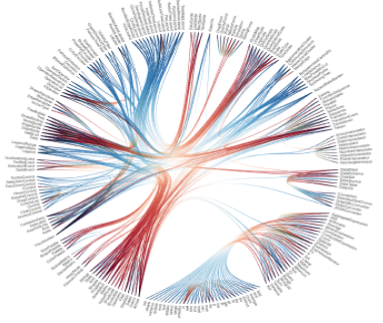
\includegraphics[width=5cm]{images/08-Benutzeroberfläche/08-Sehnendiagramm.PNG}
  \end{subfigure}
  \caption{Vorbereitete Diagramme der ersten Iteration}%
\end{figure}

Die Rückmeldungen und Diskussion am Ende der ersten Iteration, haben gezeigt, dass die direkte Visualisierung des Graphen zu unübersichtlich und nicht anschaulich ist. Ebenso ist das Sankey-Diagramm unübersichtlich und schwer zu interpretieren. Diese Diagramme sind nicht übernommen worden. Im Gegenteil dazu, wurden das Sehenendiagramm zur Visualisierung der Interaktionen und das halbe Kreisdiagramm zur Darstellung der Sitzeverteilung sehr positiv angenommen und deswegen weiter entwickelt.

In der zweiten Iteration wurden das Netzdiagramm und die Balkendiagramme integriert, die positives Feedback bekommen haben. Ebenfalls haben wir mit Box-Plots experimentiert, diese allerdings wegen der hohen Komplexität nicht weiter verfolgt.

\begin{figure}[hbt!]
    \centering
    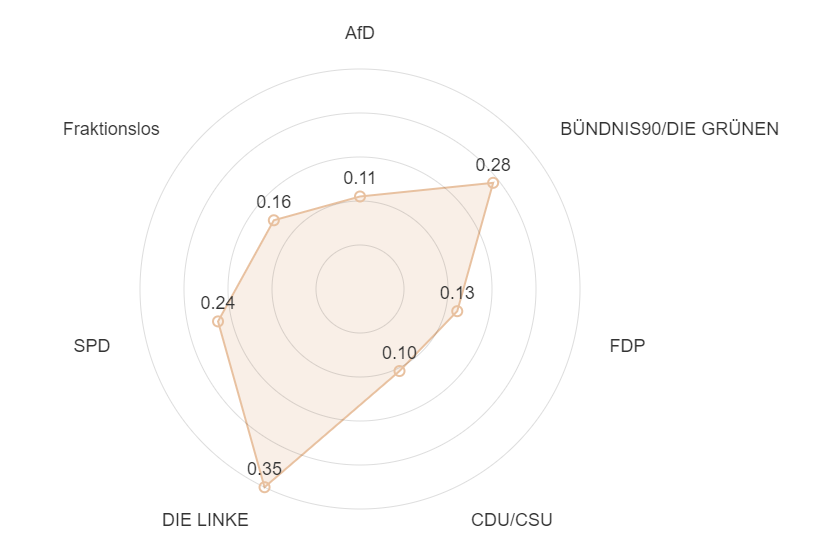
\includegraphics[width=8cm]{images/08-Benutzeroberfläche/08-Netzdiagramm.PNG}
    \caption{Eingeführtes Netzdiagramm}
\end{figure}

Nach den ersten beiden Iterationen standen die Diagrammtypen fest und wir konnten mit den einbetten der Diagramme in die Oberfläche beginnen. Dazu wurden die Diagramme in ein Storyboard eingebunden und mit Texten beschrieben. In den letzten Iterationen wurden Kleinigkeiten, wie die Texte und die Farben, abgestimmt um zum finalen Produkt zu gelangen.
\section{Implementierung}\label{sec:08_05_implementierung}

\subsection{Technologien}
Die Benutzeroberfläche ist eine Single-Page-App, die hauptsächlich in React mit TypeScript geschrieben wurde. TypeScript typisiert JavaScript und ermöglicht die Vorteile einer typisierten Sprache. React Router DOM wurde verwendet, um die Navigation ohne eine Webseitenaktualisierung zu implementieren. Datenfluss und -verwaltung wurden mit Redux und Redux Sagas ermöglicht.  Durch den Einsatz der vordefinierten UI-Elemente von Ant Design und Bootstrap konnten wir eine einheitliche Designsprache beibehalten. Letztlich wurden mit nivo die dynamischen und animierten Grafiken erstellt.


\begin{figure}[hbt!]%
  \centering
  
\includegraphics[width=14cm]{images/08-Benutzeroberfläche/08-frontend-framework-icons.PNG}
  \caption{Eine Übersicht über alle verwendeten Technologien, Werkzeuge und Bibliotheken}%
\end{figure}



\subsubsection{React}
React basiert auf dem sogenannten Komponentenmuster (engl. \dq component pattern\dq), in der jedes Element einer Webseite einer \dq stateless\dq Komponente entspricht. \dq Stateless\dq Komponenten sind wiederverwendbare Webseiten Elemente, welche keinen eigenen Status, Daten oder Inhalt besitzen. Sie dienen lediglich für die funktionale Transformationen von Eingabedaten.\cite{ReactDoc} Zudem kann jede Komponente ebenfalls eine Tochterkomponente besitzen.

Die Daten und Komponenten werden von sogenannten Container verwaltet. Ein Container aggregiert die benötigten Komponenten und sorgt für den Datenfluss.

\begin{figure}[hbt!]%
  \centering
  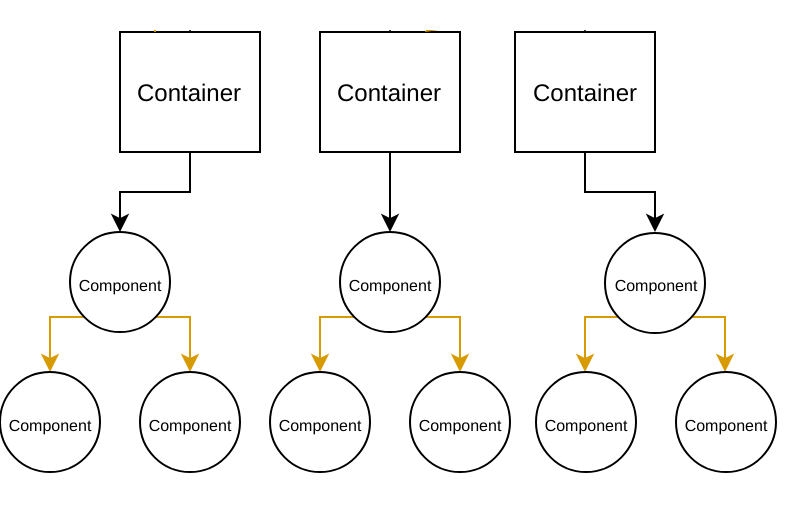
\includegraphics[width=10cm]{images/08-Benutzeroberfläche/08-react-component.PNG}
  \caption{Die Visualisierung vom Datenfluss im Komponentenmuster. Eine Menge von Container besitzen Komponenten welche Daten erhalten und weiter an den Tochterkomponenten übergeben von \cite{itnext18}}%
\end{figure}

\subsubsection{Redux und Redux Sagas}
Redux und Redux-Sagas wurde für den Datenfluss und -verwaltung verwendet. 

Redux dient als ein globaler Speicherort für Informationen. Daher wird Redux oftmals auch als Redux Store bezeichnet. Container greifen auf den Redux Store zum um entweder Daten zu erhalten oder zu verändern. Dabei können Container sogenannte Actions ausführen, um Daten zu erhalten. Mithilfe von Reducer können Daten vorselektiert oder verändert werden. 

\begin{figure}[hbt!]%
  \centering
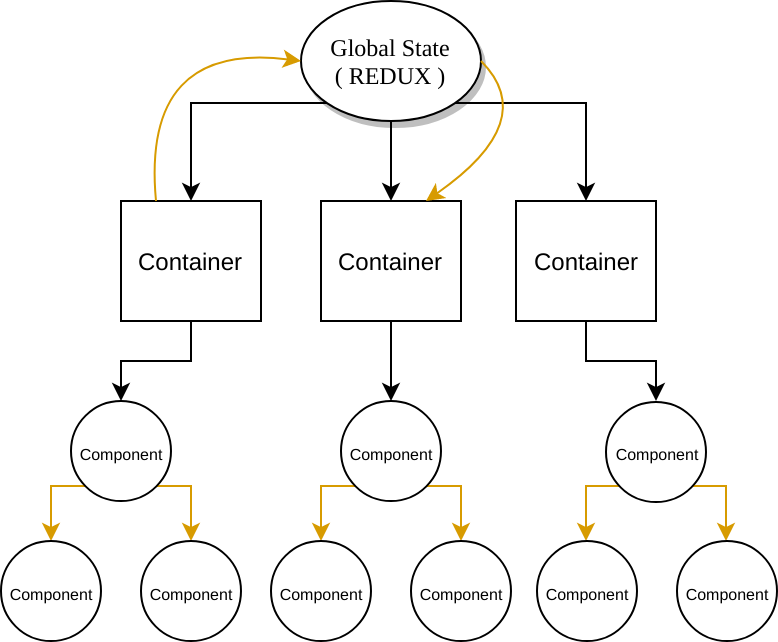
\includegraphics[width=10cm]{images/08-Benutzeroberfläche/08-react-redux.png}
  \caption{Die Visualisierung vom Datenfluss im Komponentenmuster mit Redux von \cite{itnext18}}%
\end{figure}

Die Informationen im Redux Store müssen jedoch erst von einem Server angefordert werden. Dieser Vorgang ist jedoch asynchron und gibt keine Informationen über den Status des Prozesses zurück. Beispielsweise es ist nicht bekannt ob der Server die Daten verarbeitet oder ob der Prozess fehlgeschlagen ist. Der Anwender hingegen möchte wissen, ob Daten gerade verarbeitet werden. Um dies zu ermöglichen, wurde Redux-Sagas eingesetzt. Redux-Sagas ist eine Middleware, die sich zwischen der Benutzeroberfläche und dem Redux Store befindet. Wenn die Benutzerfläche eine Action ausführt, wird die Middleware Daten vom Server anfordern und dem Reducer weitergeben. Der Reducer wiederum bearbeitet die Daten und speichert sie im Redux Store. 

\begin{figure}[hbt!]%
  \centering
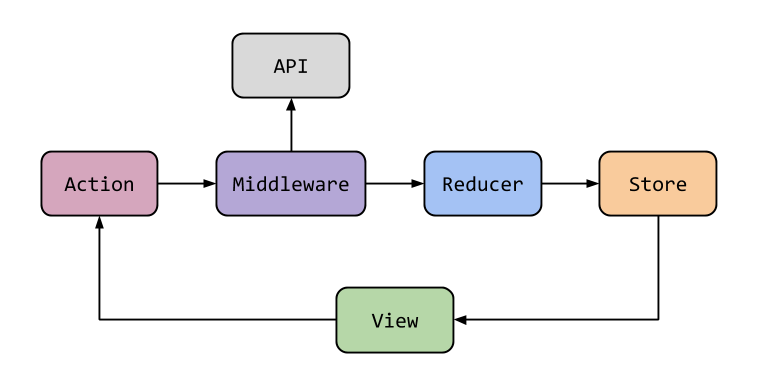
\includegraphics[width=10cm]{images/08-Benutzeroberfläche/08-redux-middleware-diagram.png}
  \caption{Die Visualisierung vom Datenfluss mit Redux und Redux-Sagas von \cite{scalac19}. Die View ist die Benutzeroberfläche, welche eine Action ausführt und den Prozess startet.}%
\end{figure}



\subsubsection{Ant Design, Bootstrap und nivo}
Ant Design, Bootstrap und nivo sind sogenannte UI-Komponenten-Bibliotheken, Bibliotheken die vorgefertigte UI-Komponenten wie Buttons, Eingaben, Dialoge etc. bereitstellen. Sie dienen als Bausteine für Layouts und können modular verwendet werden. Jede Bibliothek hat ihre eigene Designsprache und damit ein charakteristisches Aussehen. Sie können jedoch in der Regel bis zu einem gewissen Grad angepasst werden.

Für Sentiment of Bundestag wurden Ant Design, Bootstrap und nivo verwendet. Ant Design wurde von der Firma Ant Design entworfen und stellt allgemeine UI-Komponenten wie Buttons, Tabellen und co. in der firmeninternen Designsprache zur Verfügung. Bootstrap stellt ähnliche Komponenten wie Ant Design zur Verfügung, allerdings in der Designsprache der Firma Twitter. Bei Nivo handelt es sich um ein Open-Source-Projekt, das vorgefertigte Diagramme anbietet, die mit d3.js und anderen React-Frameworks implementiert sind. Ihr Vorteil ist, dass die Diagramme animiert und für mobile Geräte optimiert sind. 

\section{Zusammenfassung und Ausblick}\label{sec:08_05_zusammenfassung}
Durch die unterschiedlichen angewandten Methoden und die verwendeten Frameworks und Bibliotheken konnten wir viel Neues kennen lernen. Rückblickend konnten wir in diesem Semester eine solide und gut vorzeigbare Benutzeroberfläche für unser Informationssystem schaffen. Wir haben sehr viel positives Feedback erhalten und bei der Live-Demo und in den vorangegangenen Präsentationen hat die Webseite wie geplant funktioniert.

\begin{figure}[hbt!]
    \centering
    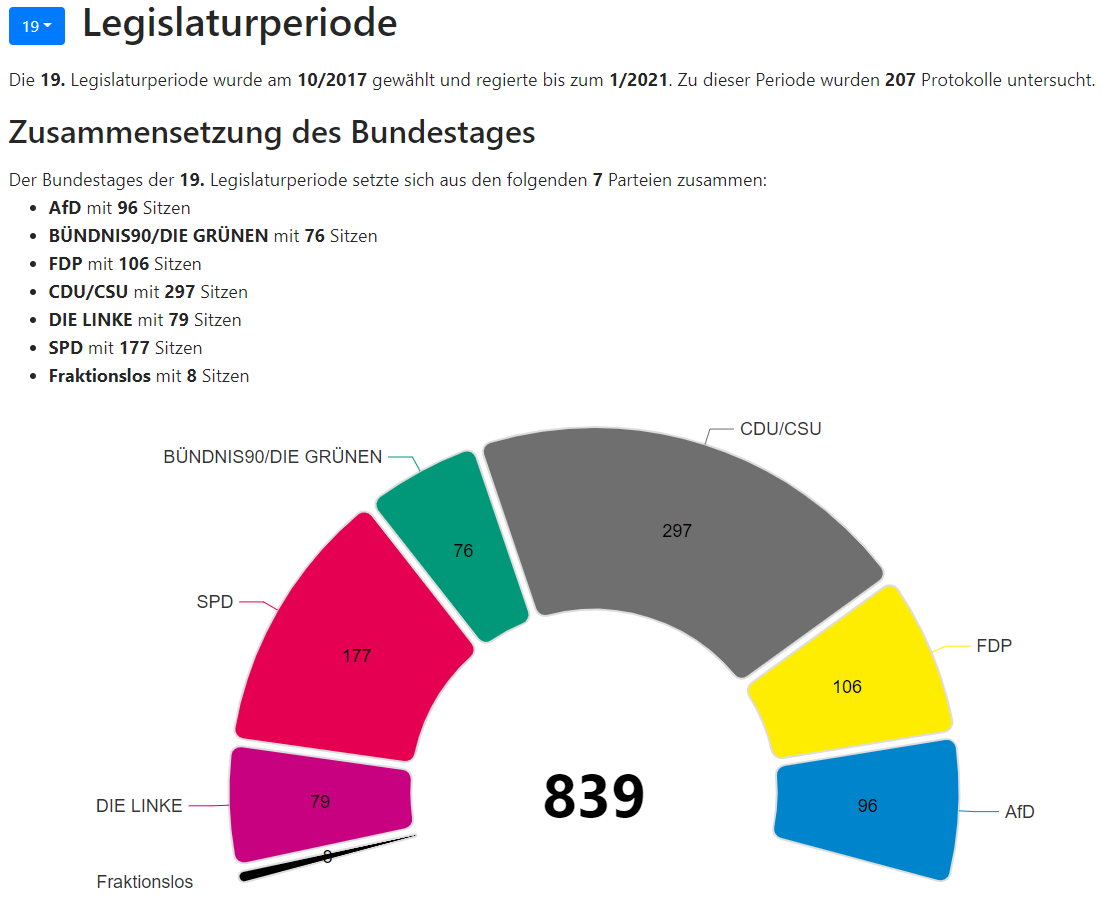
\includegraphics[width=14cm]{images/08-Benutzeroberfläche/08-Legislaturperioden.PNG}
    \caption{Screenshot aus der Benutzeroberfläche}
\end{figure}

Ein Aspekt den wir zu Beginn des Semesters unterschätzt haben war die Abhängigkeit von den vorangehenden Gruppen. Diese führte zu Zeitproblemen, Koordinationsaufwand und Problemen bei der Entwicklung. Diese Herausforderungen konnten wir nur im Team durch Zusammenarbeit und durch direkte Kommunikation mit den anderen Gruppen lösen.
Alles in Allem sind wir mit dem Projekt sehr Zufrieden. Sowohl der Lernerfolg in diesem Semester als auch das dabei entstandenen Produkt sind überzeugend. Wir hoffen sehr, dass das Projekt in Zukunft fortgeführt wird und andere Studierende den Design Thinking Prozess und die Entwicklung fortführen.

\subsection{Erreichbarkeit}
Die Webseite kann, für derzeit unbestimmte Zeit, unter http://infosys7.f4.htw-berlin.de/ erreicht werden. Sollte dieser Link nicht mehr erreichbar sein, bitte wenden Sie sich an Prof. Dr. rer. nat. Thomas Hoppe.




\pagenumbering{roman}
\setcounter{page}{6}

\printbibliography[title={Literaturverzeichnis}]
\addcontentsline{toc}{chapter}{Literaturverzeichnis}
\newpage

\printglossaries
\addcontentsline{toc}{chapter}{Glossar}
\newpage

\end{document}